% ----------------------------------------------------------
%% Capitulo5Resultados.tex
% ----------------------------------------------------------
% Resultados Numericos
% ----------------------------------------------------------
\chapter[Resultados]{Resultados Numéricos}
\label{Cap_ResultadosNumericos}

Neste capítulo, apresentam-se os resultados numéricos obtidos para verificar a implementação do código com os métodos apresentados no Capítulo \ref{Cap_MetodosNumericos}. O objetivo principal desta análise é avaliar a ordem numérica dos métodos utilizados no código. Além disso, destacamos a relevância do MMS para escoamentos de fluidos viscoelásticos, conforme introduzido neste estudo, como uma ferramenta confiável para a verificação e validação de outros códigos dentro do mesmo domínio de pesquisa.

\section{\textit{Softwares} utilizados e estrutura do código}\label{sec_ResultadosNumericos_software}

Para determinar os termos fonte essenciais no âmbito do MMS, utilizamos as capacidades do \textit{software Mathematica} \cite{Mathematica}, desenvolvido pela \textit{Wolfram Research}, amplamente reconhecido por suas funcionalidades em álgebra computacional e cálculos simbólicos.

O código principal foi implementado em \textit{Fortran77} \cite{Fortran97}, linguagem escolhida por sua eficiência em simulações numéricas de alto desempenho. Os procedimentos de pós-processamento e análise gráfica dos resultados foram conduzidos no ambiente \textit{MatLab}, explorando suas ferramentas de visualização e análise de dados científicos. O código principal segue a seguinte sequência de execução dos métodos numéricos: A simulação começa com a definição das condições iniciais e de contorno para cada variável $\varphi$, além de especificar o erro máximo admissível, denotado como $Er_{\infty}$, que determina quando as condições de estado estacionário são atingidas. Em seguida, o algoritmo continua em etapas iterativas, desde que $t$ permaneça menor que $t_f$ ou até que o critério pré-definido $Er_{\varphi} \geq Er_{\infty}$ seja atendido. Em cada iteração, as seguintes operações são executadas, considerando que a variável $\varphi$ representa, para efeitos de simplicidade, as variáveis $\omega_{z}$, $T^{xx}$, $T^{xy}$ e $T^{yy}$ simultaneamente: 1) Calcular os quatro estágios do método de Runge-Kutta para $\varphi$ (\autoref{eq_rk_4order}); 2) Determinar $\Psi$ resolvendo a equação de Poisson; 3) Aplicar a filtragem espacial em $\varphi$ (Equação (\autoref{filtragem_espacial}); e 4) Calcular as componentes de velocidade $u$ e $v$ utilizando o campo $\Psi$ obtido (\autoref{eq_Psiy_u_Psix_v}). Posteriormente, avalia-se o erro relativo $Er_{\varphi}$ e ajusta-se o passo de tempo $dt$ conforme necessário. No \autoref{code_pseudo} apresenta-se o pseudocódigo do que foi descrito.
\begin{algorithm}
\caption{Código com Runge-Kutta de quarta ordem}\label{code_pseudo}
\begin{algorithmic}[1]
\Function{main}{par.nn}
  \State Condições iniciais e de contorno para $\varphi$;
  \State Defina o valor de $Er_{\infty}$; \Comment{Erro máximo a ser alcançado no estado estacionário}
  \While {$t \leq tf$}
    \For{i}{\ 1 até }{4} 
       \State Calcula o passo $i$ do Runge-Kutta para $\varphi$ \eqref{eq_rk_4order}
       \State Calcula $\Psi$, resolvendo a equação de Poisson usando o método Multigrid;
       \State Realiza a filtragem espacial descrita em \eqref{filtragem_espacial} para $\varphi$;
       \State Calcula $u$ e $v$, usando $\Psi$  \eqref{eq_Psiy_u_Psix_v};
       \State Calcula $\omega$ na parede utilizando \eqref{parede_baixo_vortici}-\eqref{parede_direita_vortici};
    \EndFor
    \State Calcular $Er_{\varphi} = \frac{||\varphi^{n+1} - \varphi^{n}||_{\infty}}{||\varphi^{n+1}||_{\infty}}$; \Comment{Erro relativo}
    \If {$Er_{\varphi} \leq Er_{\infty}$ \textbf{e} $t \geq 0.01$}
        \State Finalizar avanço temporal
    \EndIf
    \State $t \gets t + dt $; \Comment{Passo de tempo ou incremento de tempo}
  \EndWhile
  \State Calcula o erro entre a solução numérica e analítica para $\varphi$;
\EndFunction
\end{algorithmic}
\end{algorithm}

Na etapa final deste processo, as discrepâncias entre as soluções numéricas e analíticas para cada variável $\varphi$ são comparadas para conseguir determinar . Essa comparação é feita calculando a norma $k$ para o termo de erro $e$, definido como:
\begin{align}
    &\left \|e\right \|_{k}=\left(\Delta x_{i} \Delta y_{j} \sum_{i=1}^{N_{i}}\sum_{j=1}^{N_{j}} \left |e\right |_{i,j}^{k}\right)^{1/k}, \label{norm_k}
\end{align}
onde $\Delta x_{i}$ e $\Delta y_{j}$ representam o espaçamento da malha nas direções $x$ e $y$, enquanto $N_{i}$ e $N_{j}$ são o número total de pontos nas respectivas direções, e $e$ é a diferença entre a solução manufaturada e a solução numérica. Essa fórmula permite uma avaliação quantitativa eficaz dos erros em todo o domínio computacional. Para determinar a ordem de convergência numérica, representada por $p$, adotamos o procedimento descrito por \citeonline{leveque2007finite}, que se baseia na seguinte relação logarítmica entre os erros obtidos em sucessivas resoluções de malha:
\begin{equation}\label{log_p} 
    p \approx \frac{\log\left(\frac{e_{l}}{e_{l+1}}\right)}{\log\left(\frac{h_{l}}{h_{l+1}}\right)},
\end{equation}
onde $e_{l}$ é o erro associado a espaçamento de malha $h_{l} = \max\limits_{N_i,N_j}\{\Delta x_{i};\ \Delta y_{j}\}.$ Essa abordagem permite verificar a taxa de convergência do método numérico utilizado, avaliando a relação entre os erros de discretização nas diferentes refinamentos de malha, o que é essencial para garantir a confiabilidade e precisão do código.

\section{Domínio computacional e parâmetros para a verificação}

Para todos os casos teste, considera-se o domínio $\Omega = [0;L]\times[0;H] = [0;1]\times[0;1]$, conforme ilustrado na \autoref{fig:domain}.
\begin{figure}[H]
        \centering
	\caption{Domínio computacional}\label{fig:domain}
        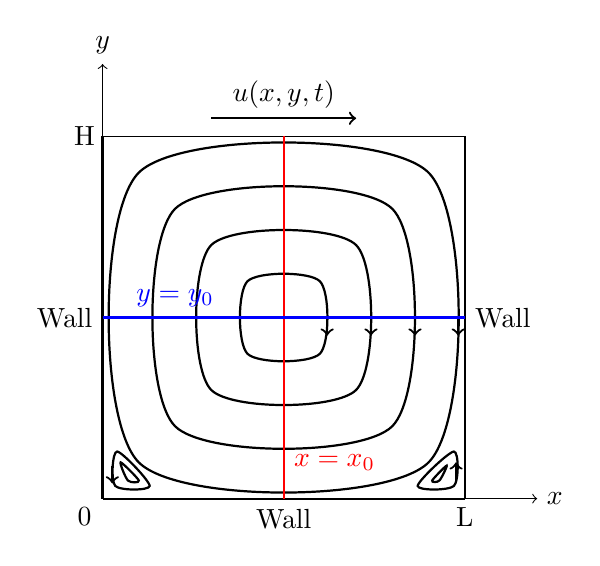
\begin{tikzpicture}[scale=4.6]
            % Eixos x e y
            \draw[->] (0,0) -- (1.2,0) node[right] {$x$};
            \draw[->] (0,0) -- (0,1.2) node[above] {$y$};
            % Desenhando o quadrado do domínio
            \draw (0,0) rectangle (1,1);
            % Desenho da tampa (lid)
            % \draw[->, thick] (0,1) -- (1,1) node[midway, above] {Lid};
            \draw[-, thick]  (0,0) -- (1,0) node[midway, below] {Wall};
            \draw[-, thick]  (0,0) -- (0,1) node[midway, left] {Wall};
            \draw[-, thick]  (1,0) -- (1,1) node[midway, right] {Wall};
            \draw[->, thick] (0.3,1.05) -- (0.7,1.05) node[midway, above] {$u(x,y,t)$};
            % Outras anotações
            \node at (-0.05,-0.05) {0};
            \node at (1,-0.05) {L};
            \node at (-0.05,1) {H};
            % Vortice central
            \draw[thick] plot[smooth cycle] coordinates {(0.1,0.9) (0.9,0.9) (0.9,0.1) (0.1,0.1)};
            \draw[thick] plot[smooth cycle] coordinates {(0.2,0.8) (0.8,0.8) (0.8,0.2) (0.2,0.2)};
            \draw[thick] plot[smooth cycle] coordinates {(0.3,0.7) (0.7,0.7) (0.7,0.3) (0.3,0.3)};
            \draw[thick] plot[smooth cycle] coordinates {(0.4,0.6) (0.6,0.6) (0.6,0.4) (0.4,0.4)};
            \draw[->, thick] (0.62,0.5) -- (0.62,0.45);
            \draw[->, thick] (0.741,0.5) -- (0.741,0.45);
            \draw[->, thick] (0.8625,0.5) -- (0.8625,0.45);
            \draw[->, thick] (0.982,0.5) -- (0.982,0.45);
            % Vortice inferrior esquerdo
            \draw[thick] plot[smooth cycle] coordinates {(0.07,0.05) (0.05,0.1) (0.1,0.05)};
            \draw[thick] plot[smooth cycle] coordinates {(0.035,0.035) (0.04,0.13) (0.13,0.035)};
            \draw[->, thick] (0.027,0.09) -- (0.027,0.042);
            % Vortice inferior direito
            \draw[thick] plot[smooth cycle] coordinates {(0.93,0.05) (0.95,0.091) (0.91,0.05)};
            \draw[thick] plot[smooth cycle] coordinates {(0.97,0.035) (0.97,0.13) (0.87,0.035)};
            \draw[->, thick] (0.976,0.05) -- (0.976,0.1);
            % Linha vertical em x = 0.5
            \draw[red, thick] (0.5, 0) -- (0.5, 1) node[pos=0.1, right] {$x = x_0$};
            % Linha horizontal em y = 0.5
            \draw[blue, thick] (0, 0.5) -- (1, 0.5) node[pos=0.2, above] {$y = y_0$};
        \end{tikzpicture}
	\fautor
\end{figure}

Por meio da utilização do Método das Soluções Manufaturadas (MMS), torna-se possível gerar uma solução de referência pré-definida, que pode ser comparada com a solução numérica obtida a partir do código computacional. Essa comparação não apenas fornece uma medida quantitativa da precisão numérica do código, mas também permite identificar possíveis discrepâncias ou desvios entre as previsões numéricas e a solução analítica conhecida. Tais desvios são quantificados pelo cálculo do erro padrão, utilizando a Equação~\eqref{norm_k} com $k = 2$, conforme descrito abaixo:
\begin{align} 
    &||e||_{2}=\left( \Delta x \Delta y \sum_{i=1}^{N_{1}}\sum_{j=1}^{N_{2}} \left |e\right |_{i,j}^{2}\right)^{1/2}.\label{norm_2}
\end{align}

A fim de avaliar o comportamento dos métodos numéricos aplicados às equações governantes para fluidos viscoelásticos, realizamos uma série de testes com diferentes modelos reológicos: UCM, Oldroyd-B, Giesekus e LPTT. Para cada um desses modelos, variamos os parâmetros relevantes, tais como o número de Reynolds ($Re$), o parâmetro $\beta_{nn}$, o número de Weissenberg ($Wi$), e, no caso dos modelos Giesekus e LPTT, o parâmetro $\alpha_G$, bem como os parâmetros adicionais $\epsilon$ e $\xi$, para os quais esses modelos são sensíveis.

Os valores desses parâmetros foram escolhidos de maneira a testar o desempenho do código numérico em uma ampla gama de condições de escoamento, desde regimes dominados por forças viscosas até aqueles com fortes efeitos elásticos. Além disso, os parâmetros $\alpha_G$, $\epsilon$ e $\xi$ foram incluídos nos modelos onde suas contribuições são significativas para capturar a complexidade do comportamento reológico. 

A Tabela \ref{tab_test_cases} resume os valores dos parâmetros usados nos casos de teste para cada modelo reológico. Essa diversidade de parâmetros foi selecionada para garantir que o método numérico seja avaliado sob diferentes cenários, verificando sua robustez e precisão em situações que incluem tanto fluidos Newtonianos quanto fluidos viscoelásticos complexos.

\begin{table}[H]
	\IBGEtab{
            \caption{Parâmetros utilizados para os testes realizados}
            \label{tab_test_cases}
        }{
            \begin{tabular}{c|cccccc}
                \toprule
                \textbf{Modelo} & $\operatorname{Re}$ & $\beta_{nn}$ & $\operatorname{Wi}$ & $\alpha_{G}$ & $\epsilon$ & $\xi$ \\ \midrule
                \textbf{UCM} & 1, 10, 100, 400 e 1000 & 0 & 1, 5 e 10 & 0 & 0 & 0 \\ \midrule
                \textbf{Oldroyd-B} & 1, 10, 100, 400 e 1000 & 0.1, 0.5, 0.9 e 1 & 1, 5 e 10 & 0 & 0 & 0 \\ \midrule
                \textbf{Giesekus} & 1, 10, 100, 400 e 1000 & 0.1, 0.5, 0.9 e 1 & 1, 5 e 10 & 0.1, 0.5 e 0.85 & 0 & 0 \\ \midrule
                \textbf{LPTT} & 1, 10, 100, 400 e 1000 & 0.1, 0.5, 0.9 e 1 & 1, 5 e 10 & 0 & 0.5 e 1 & 0.1 e 0.5 \\ \bottomrule
            \end{tabular}
        }{
		\fdadospesquisa
	}
\end{table}

Para garantir a estabilidade e a acurácia das simulações, foi adotado um passo de tempo fixo $\Delta t = 10^{-5}$, enquanto os critérios de convergência dos esquemas iterativos foram definidos com tolerância de erro de $10^{-6}$ para as variáveis principais, como função corrente, vorticidade e com as componentes do tensor de tensão. Esses valores foram escolhidos com base em testes preliminares que demonstraram bom compromisso entre precisão numérica e custo computacional.

As Figuras~\ref{U_m_u_sol_num_case1map2} e \ref{T_m_u_sol_num_case1map2} apresentam as soluções manufaturadas em regime de estado estacionário para os campos de velocidade, vorticidade, função de corrente e componentes do tensor de tensão. Essas visualizações permitem verificar qualitativamente as soluções analíticas utilizadas através do Método da Solução Manufaturada, fornecendo uma base gráfica que complementa a análise quantitativa dos erros, a serem realizadas nas seções a seguir, e permite confirmar a coerência dos padrões de escoamento e das distribuições de tensões com os resultados esperados para o problema físico modelado.

\begin{figure}[H]
        \centering
        \caption{Soluções manufaturadas no regime de estado estacionário para o campo de velocidades $(\overline{u},\tilde{v})$, vorticidade $(\tilde{\omega_{z}})$ e função de corrente $(\tilde{\psi})$, considerando $\beta_{nn}=0.1$ e $a = 0.05$ em $t=0.1$}
        \label{U_m_u_sol_num_case1map2}
        \begin{subfigure}[b]{.47\textwidth}
            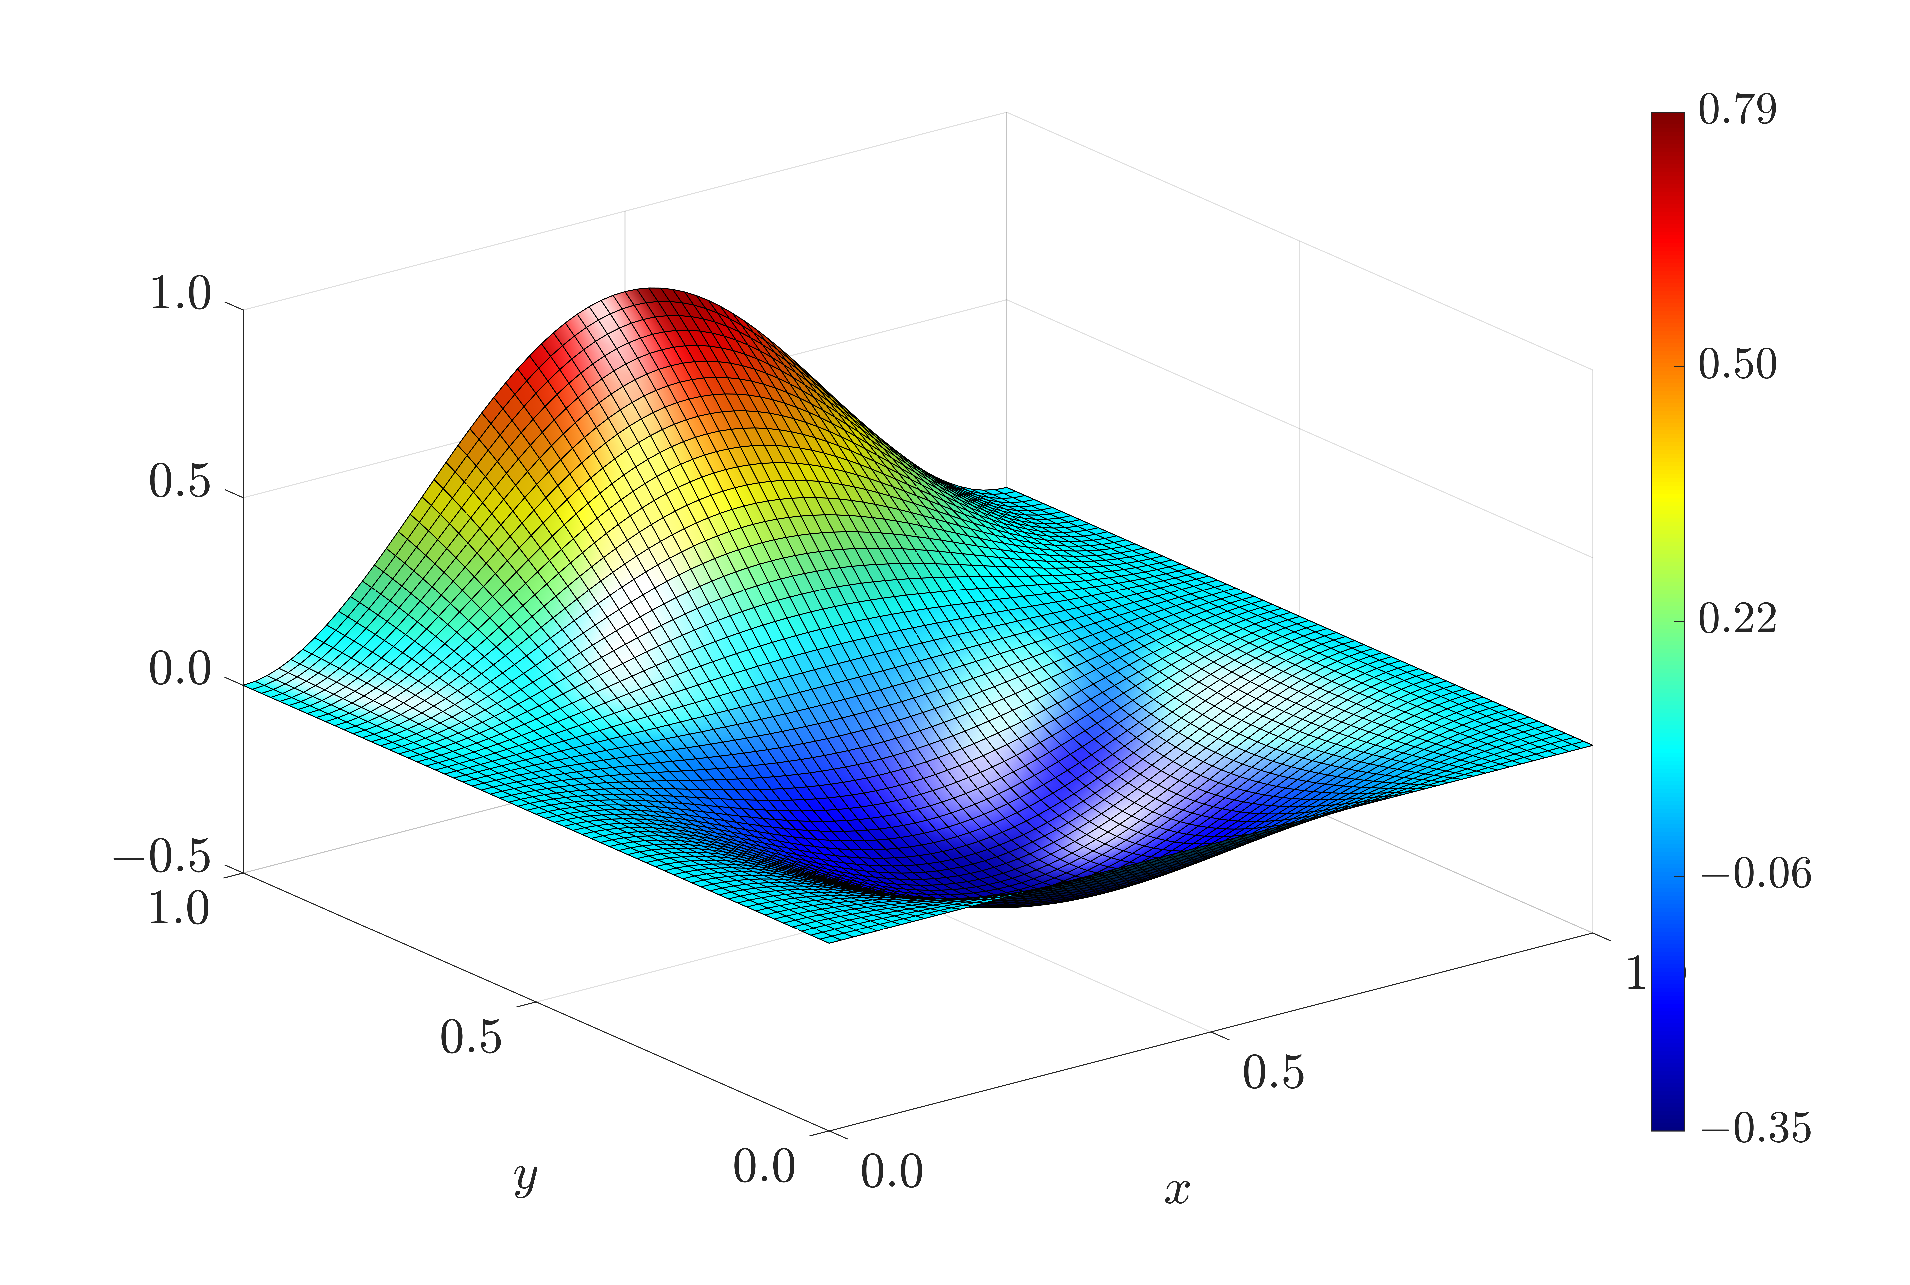
\includegraphics[width=\textwidth]{figures/Case12/UCM/Solutions/Exact_Surf_NormErr_2nd_Betann_0.1_Re_1_Wi_1_epsilon_0_xi_0_alphaG_0_Dt_1e-06_at_0.05_tipsim_1_MMS_12_U.eps}
            \caption{$\overline{u}$\label{fig_solexauCase1}}
        \end{subfigure}
        \vspace{0.2cm}
        \begin{subfigure}[b]{.47\textwidth}
            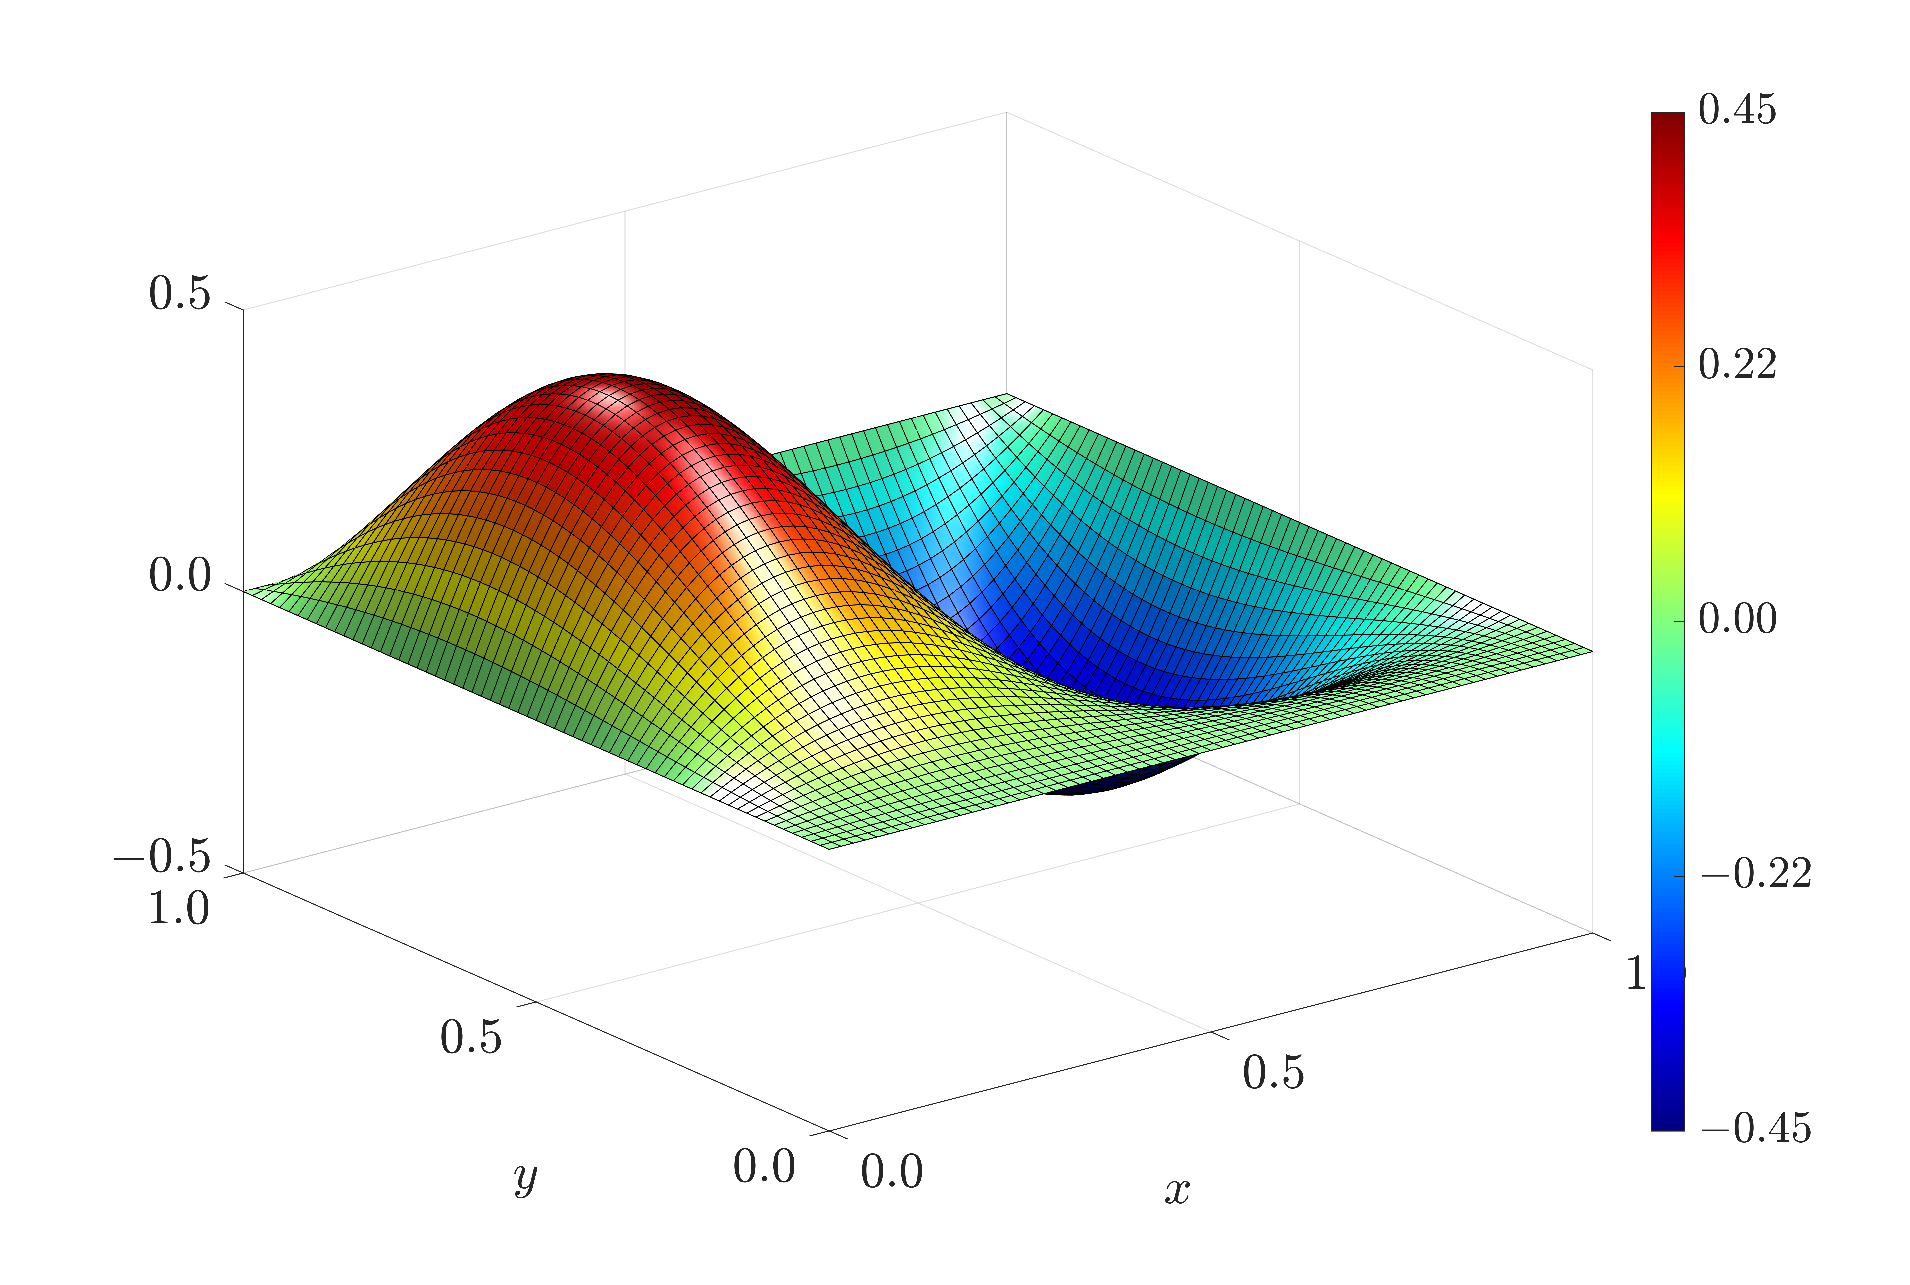
\includegraphics[width=\textwidth]{figures/Case12/UCM/Solutions/Exact_Surf_NormErr_2nd_Betann_0.1_Re_1_Wi_1_epsilon_0_xi_0_alphaG_0_Dt_1e-06_at_0.05_tipsim_1_MMS_12_V.eps}
            \caption{$\widetilde{v}$\label{fig_solexavCase1}}
        \end{subfigure}
        \begin{subfigure}[b]{.47\textwidth}
            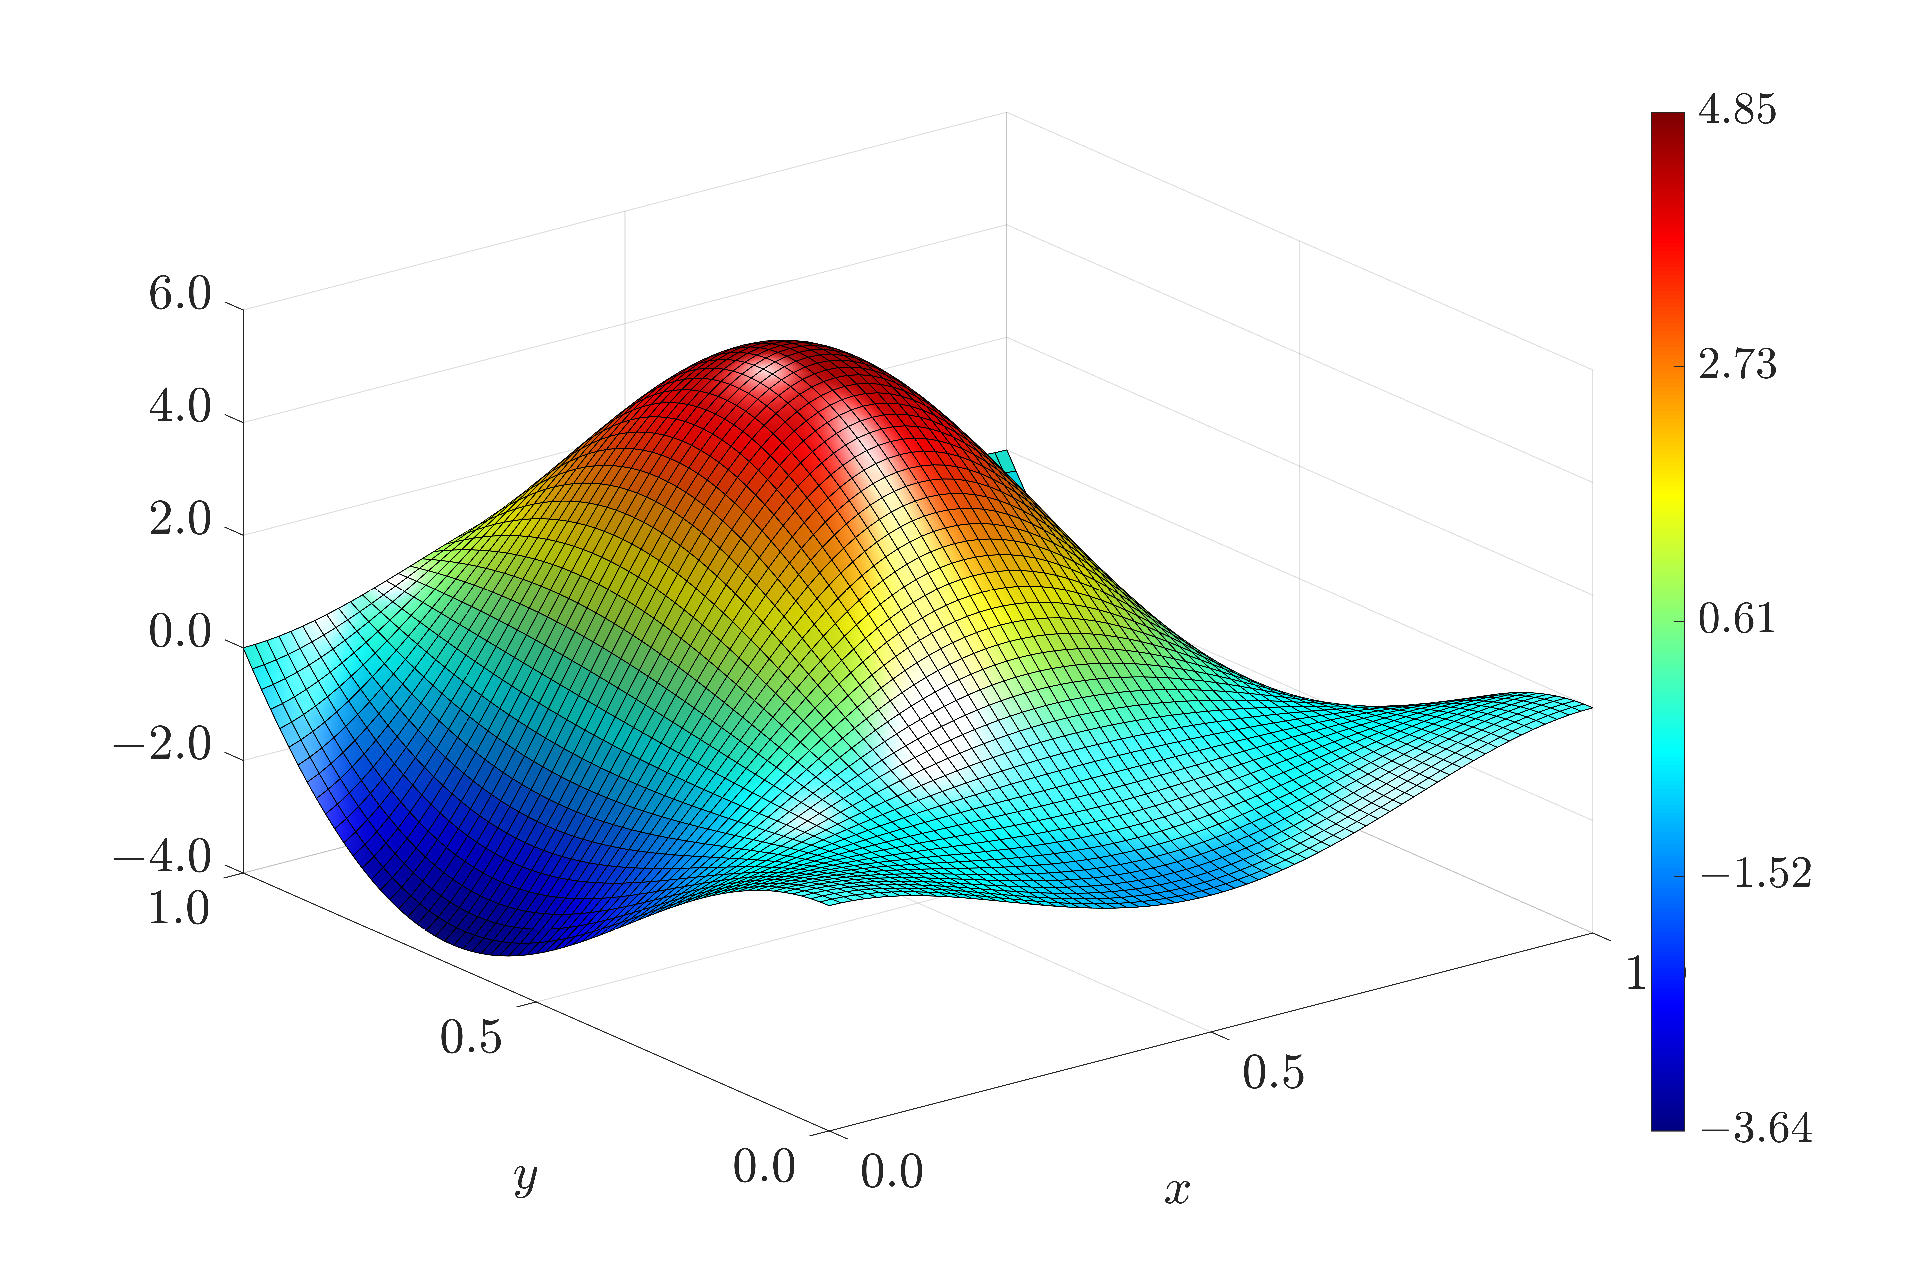
\includegraphics[width=\textwidth]{figures/Case12/UCM/Solutions/Exact_Surf_NormErr_2nd_Betann_0.1_Re_1_Wi_1_epsilon_0_xi_0_alphaG_0_Dt_1e-06_at_0.05_tipsim_1_MMS_12_Wz.eps}
            \caption{$\widetilde{\omega_{z}}$\label{fig_solexawzCase1}}
        \end{subfigure}
        \vspace{0.2cm}
        \begin{subfigure}[b]{.47\textwidth}
            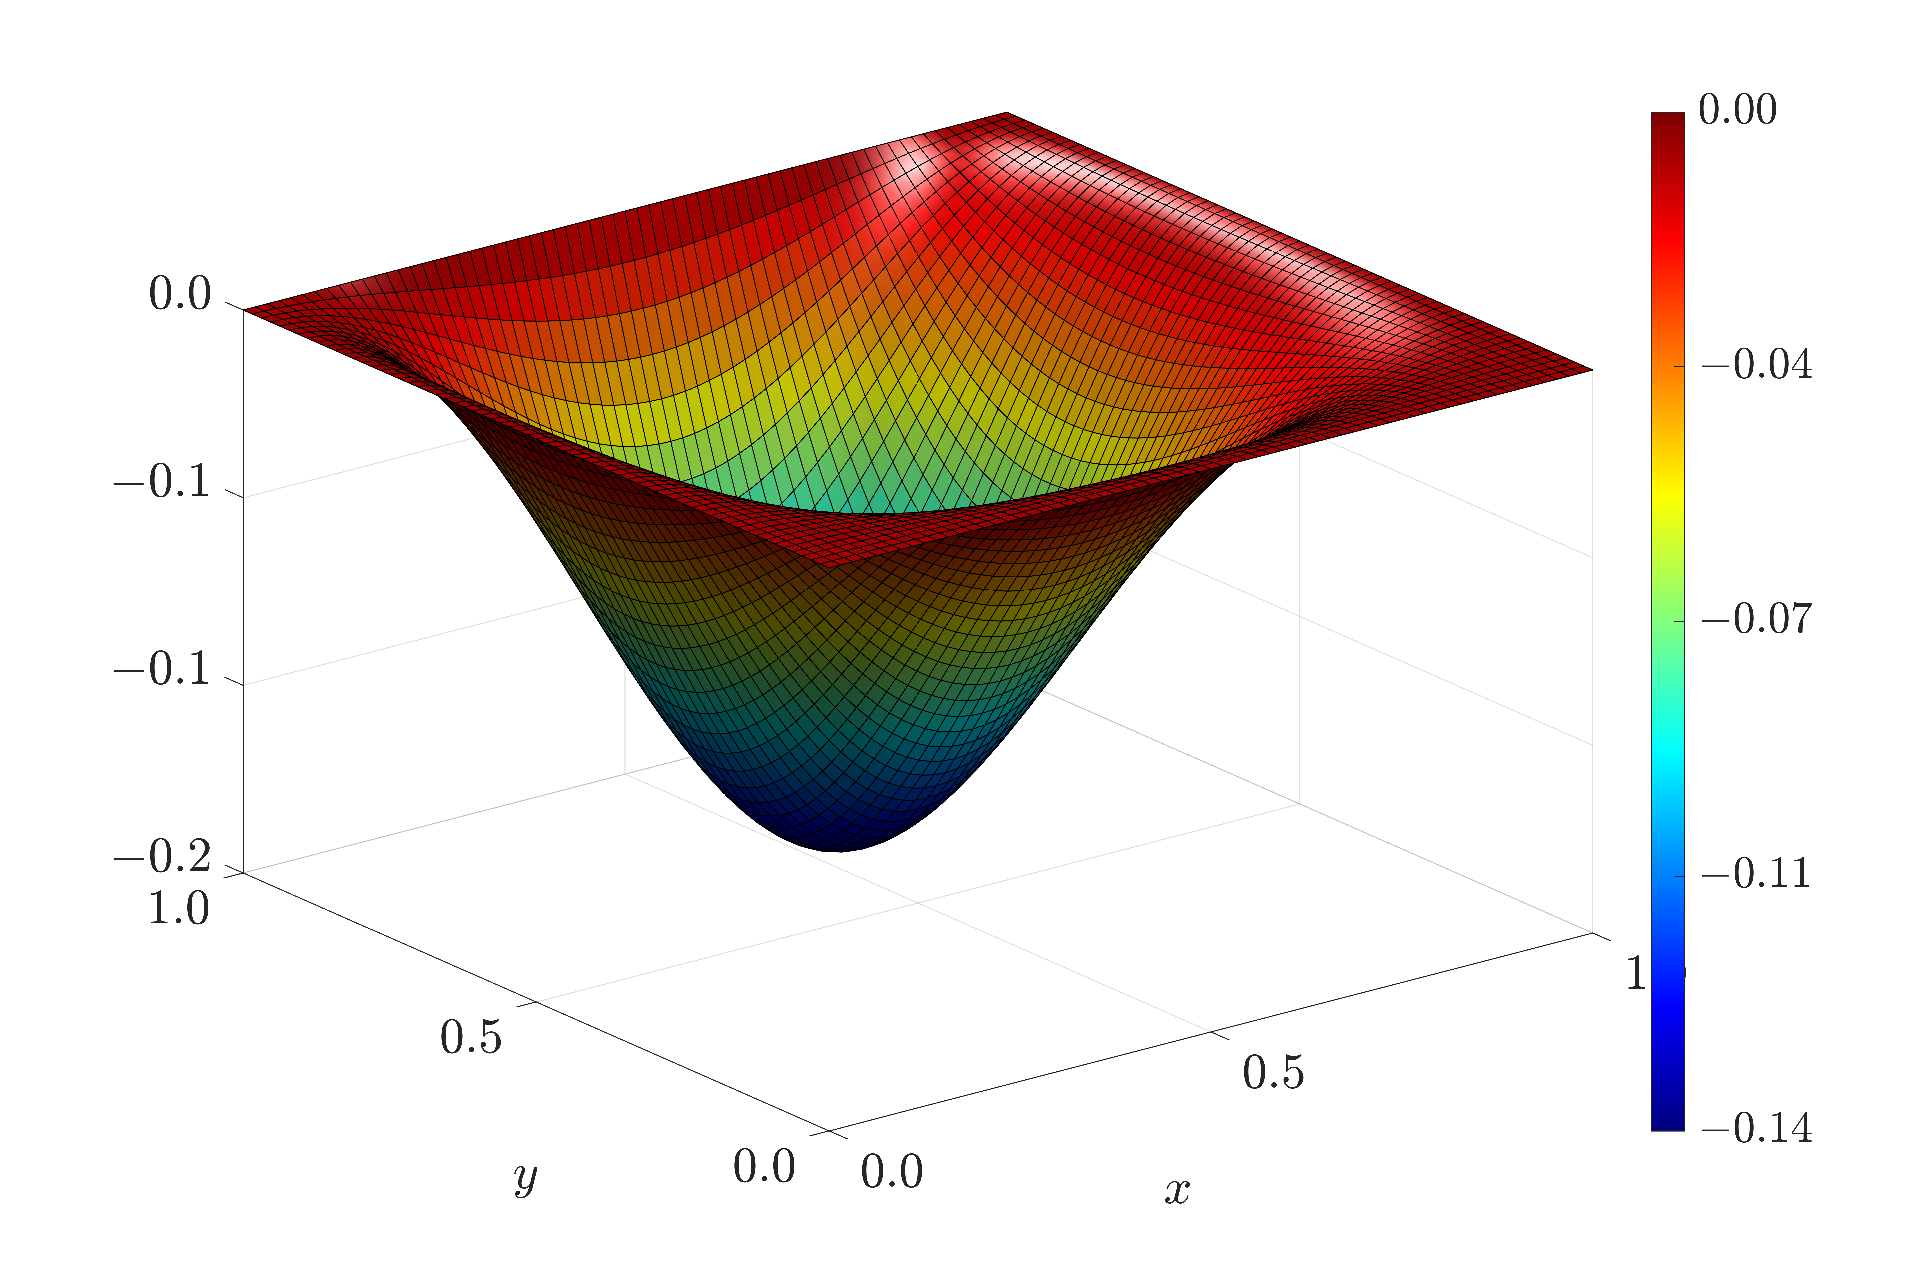
\includegraphics[width=\textwidth]{figures/Case12/UCM/Solutions/Exact_Surf_NormErr_2nd_Betann_0.1_Re_1_Wi_1_epsilon_0_xi_0_alphaG_0_Dt_1e-06_at_0.05_tipsim_1_MMS_12_Psi.eps}
            \caption{$\widetilde{\psi}$\label{fig_solexapsiCase1}}
        \end{subfigure}
        \fdadospesquisa
\end{figure}

\begin{figure}[H]
        \centering
	\caption{Soluções manufaturadas no regime de estado estacionário para os tensores, considerando $\beta_{nn}=0.1$ e $a = 0.05$ em $t=0.1$}
        \label{T_m_u_sol_num_case1map2}
        \begin{subfigure}[b]{.47\textwidth}
            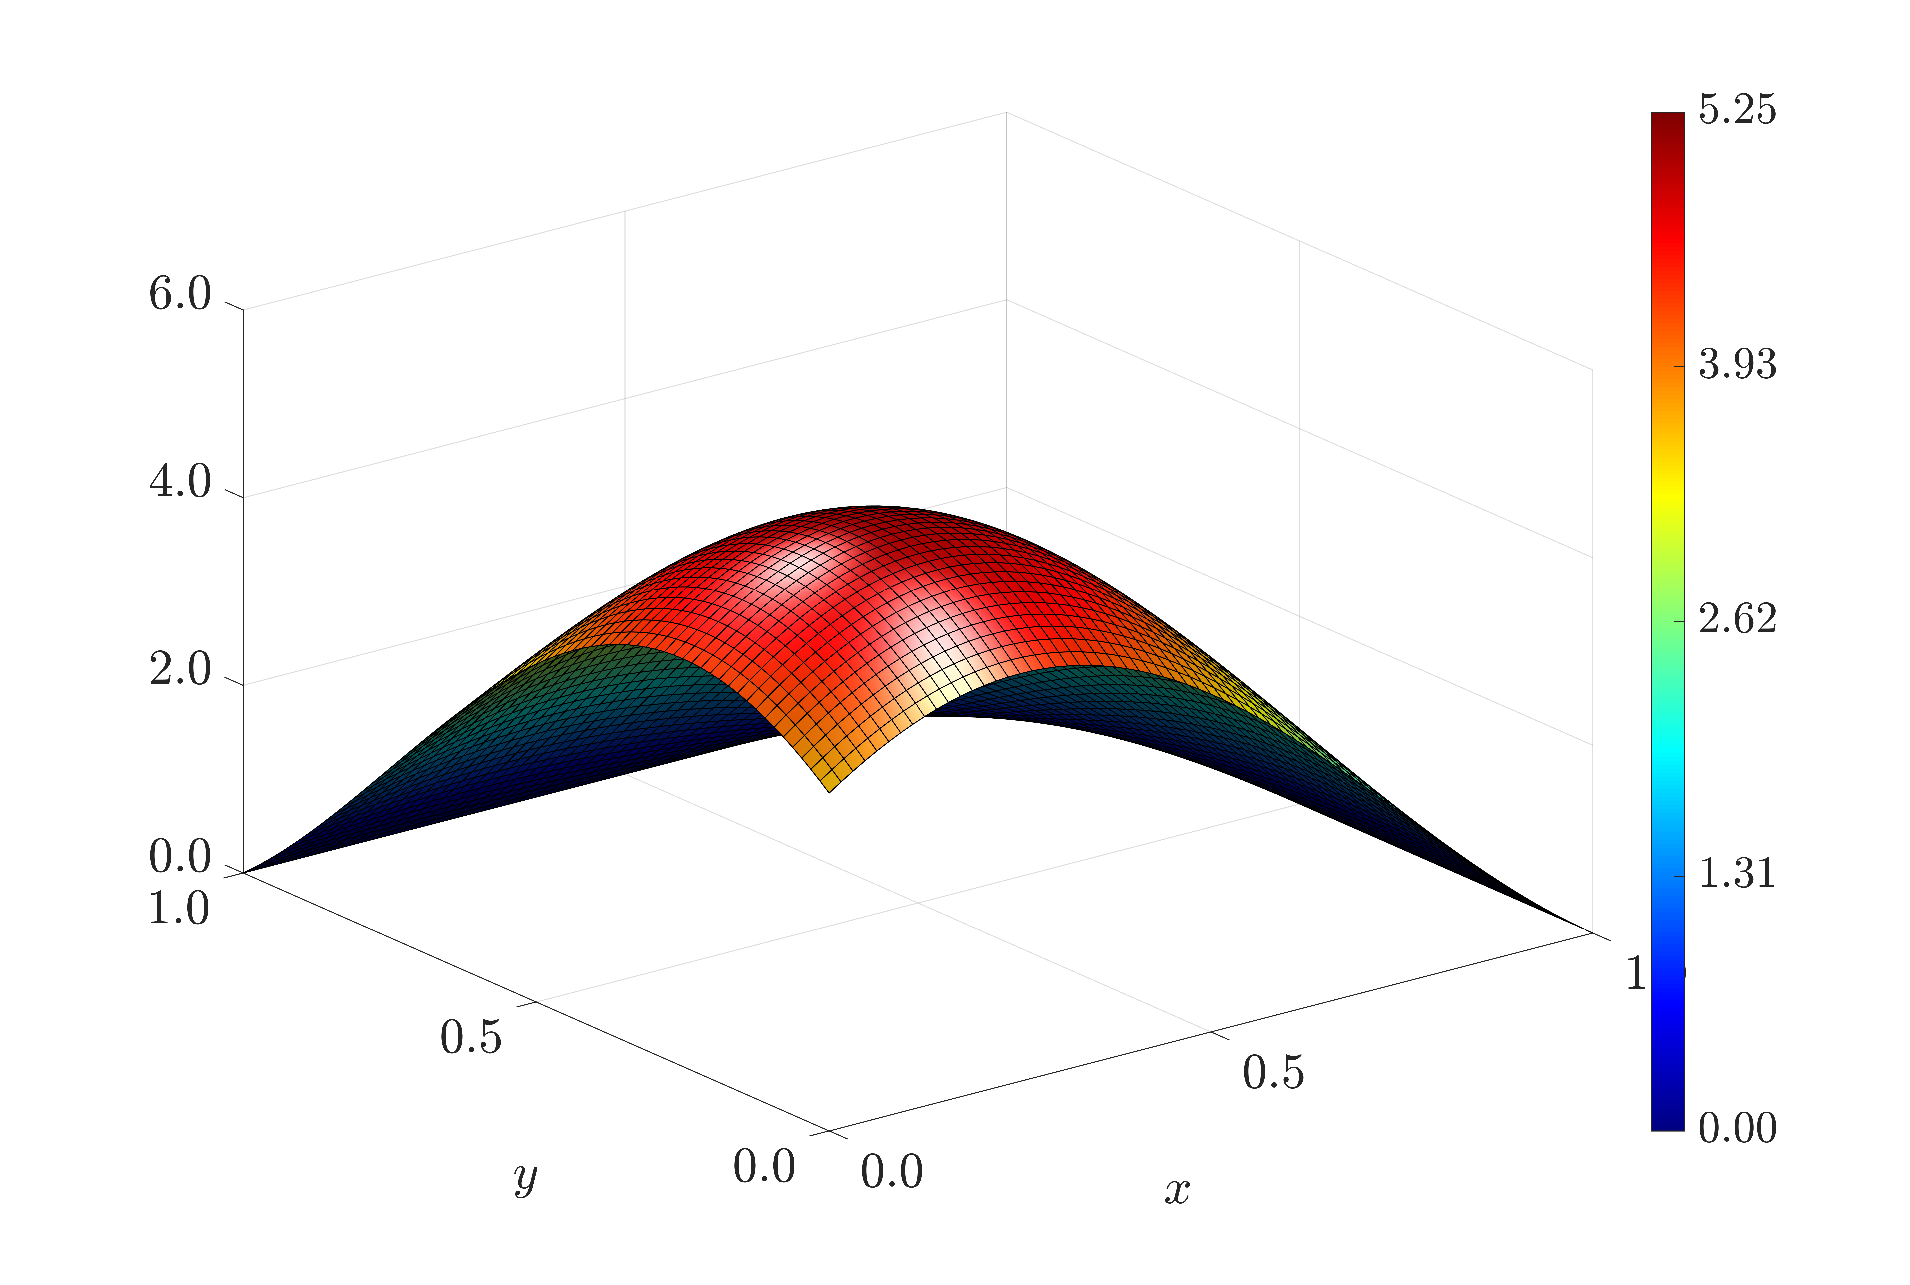
\includegraphics[width=\textwidth]{figures/Case12/UCM/Solutions/Exact_Surf_NormErr_2nd_Betann_0.1_Re_1_Wi_1_epsilon_0_xi_0_alphaG_0_Dt_1e-06_at_0.05_tipsim_1_MMS_12_Txx.eps}
            \caption{$\overline{T}_{xx}$}
            \label{fig_solexaTxxCase1}
        \end{subfigure}
        \vspace{0.2cm}
        \begin{subfigure}[b]{.47\textwidth}
            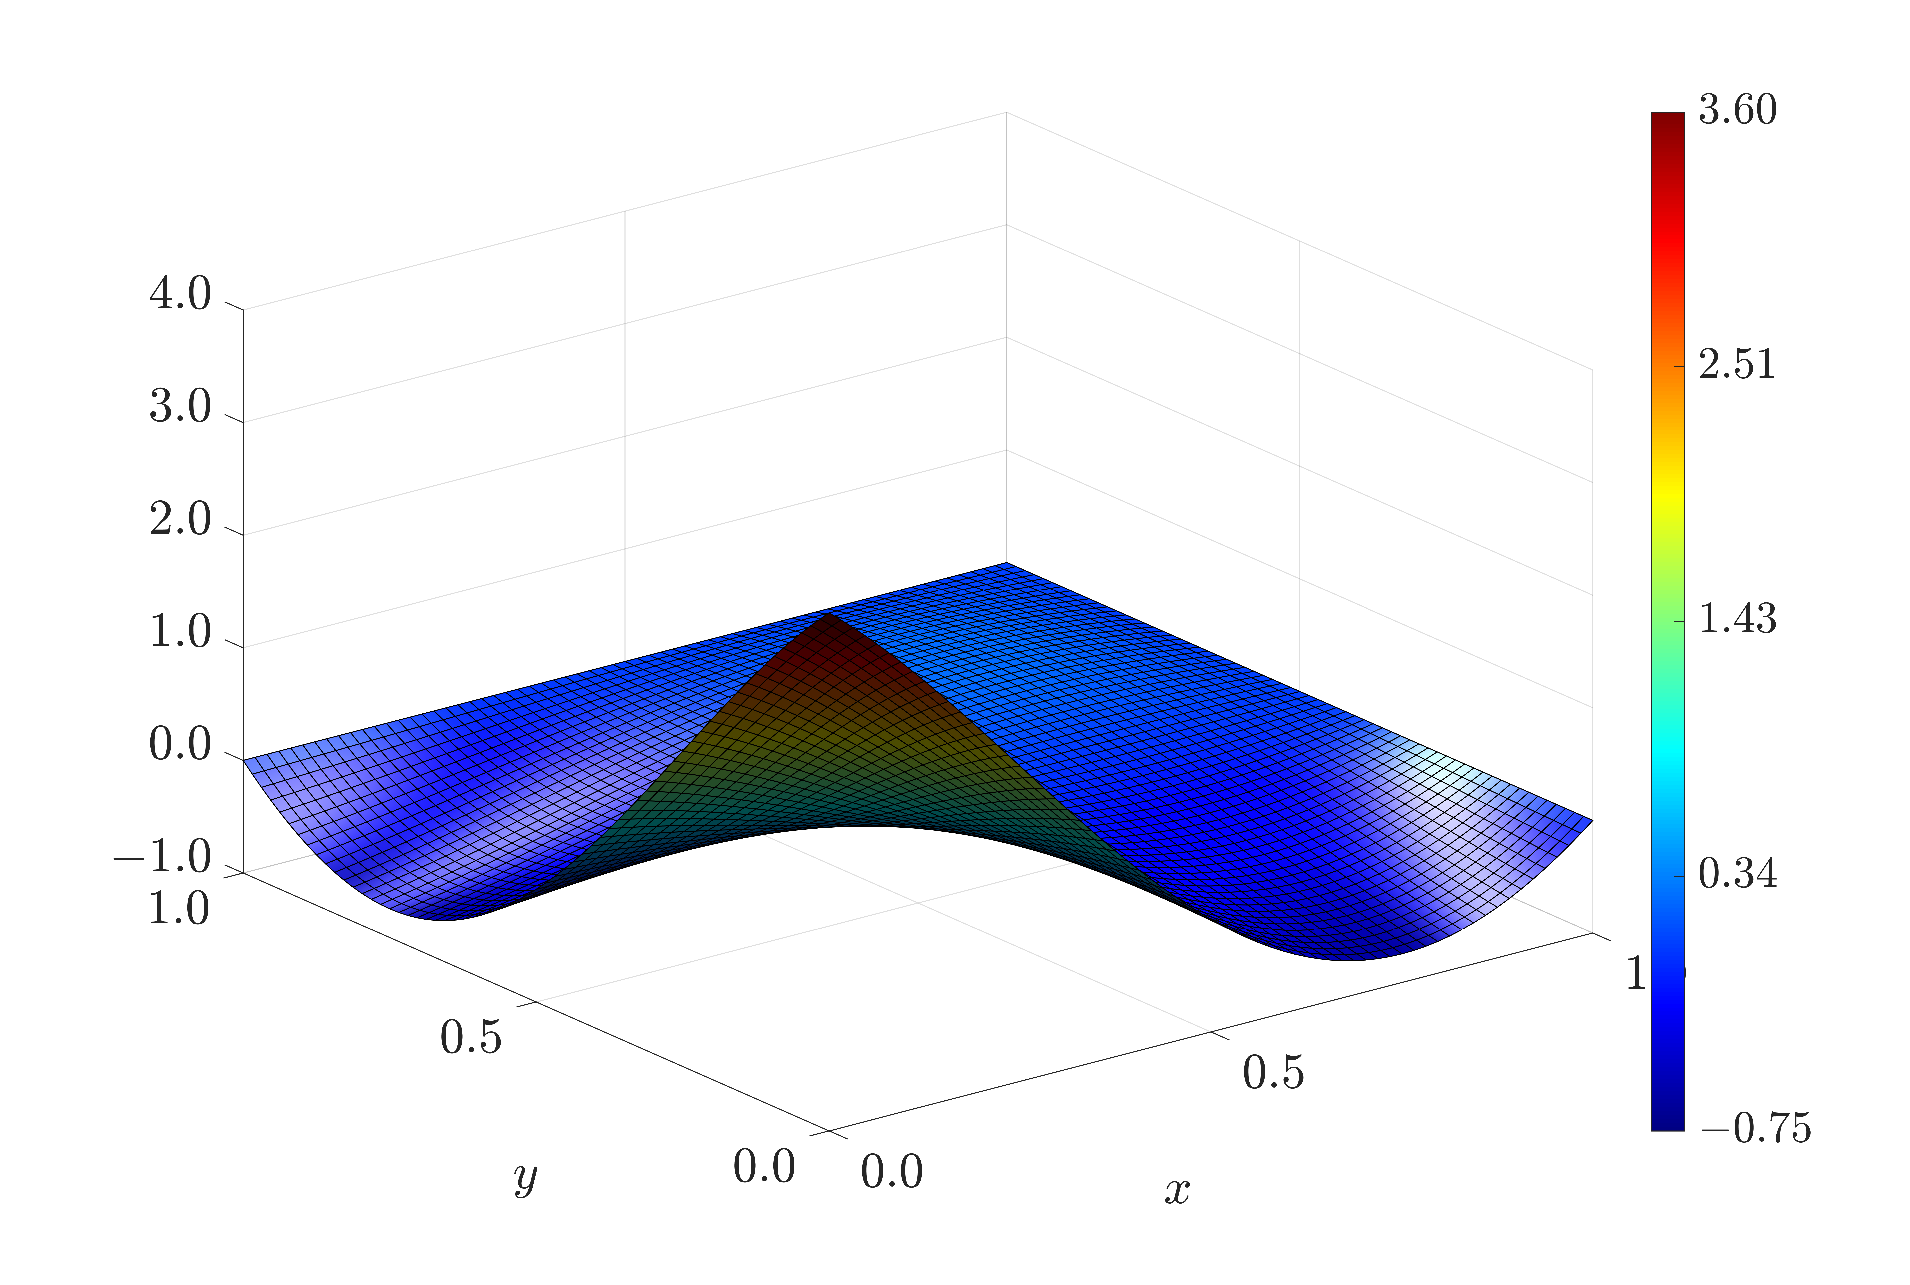
\includegraphics[width=\textwidth]{figures/Case12/UCM/Solutions/Exact_Surf_NormErr_2nd_Betann_0.1_Re_1_Wi_1_epsilon_0_xi_0_alphaG_0_Dt_1e-06_at_0.05_tipsim_1_MMS_12_Txy.eps}
            \caption{$\overline{T}_{xy}$}
            \label{fig_solexaTxyCase1}
        \end{subfigure}
        \begin{subfigure}[b]{.47\textwidth}
            \includegraphics[width=\textwidth]{figures/Case12/UCM/Solutions/Exact_Surf_NormErr_2nd_Betann_0.1_Re_1_Wi_1_epsilon_0_xi_0_alphaG_0_Dt_1e-06_at_0.05_tipsim_1_MMS_12_Tyy.eps}
            \caption{$\overline{T}_{yy}$}
            \label{fig_solexaTyyCase1}
        \end{subfigure}
	\fdadospesquisa
\end{figure}

As Figuras~\ref{fig_U_m_u_sol_num_case1streamline2} e \ref{fig_T_xxxyyy_sol_num_case1streamline2} apresentam as linhas de corrente das soluções manufaturadas no regime de estado estacionário, utilizando os parâmetros $\beta_{nn} = 0.1$ e $a = 0.05$. Além disso, essas figuras mostram as linhas de corrente juntamente com um mapa de contorno das soluções manufaturadas no mesmo regime, confirmando que o padrão de escoamento das soluções segue o comportamento típico do problema da cavidade com tampa deslizante, conforme apresentado em \citeonline{bruneau20062d}.
\begin{figure}[H]
        \centering
        \caption{Mapas de cores das soluções manufaturadas no regime de estado estacionário para o campo de velocidades $(\overline{u},\tilde{v})$, vorticidade $(\tilde{\omega_{z}})$ e função de corrente $(\tilde{\psi})$, considerando $a = 0.05$ em $t=0.1$}
        \label{fig_U_m_u_sol_num_case1streamline2}
        \begin{subfigure}[b]{.47\textwidth}
            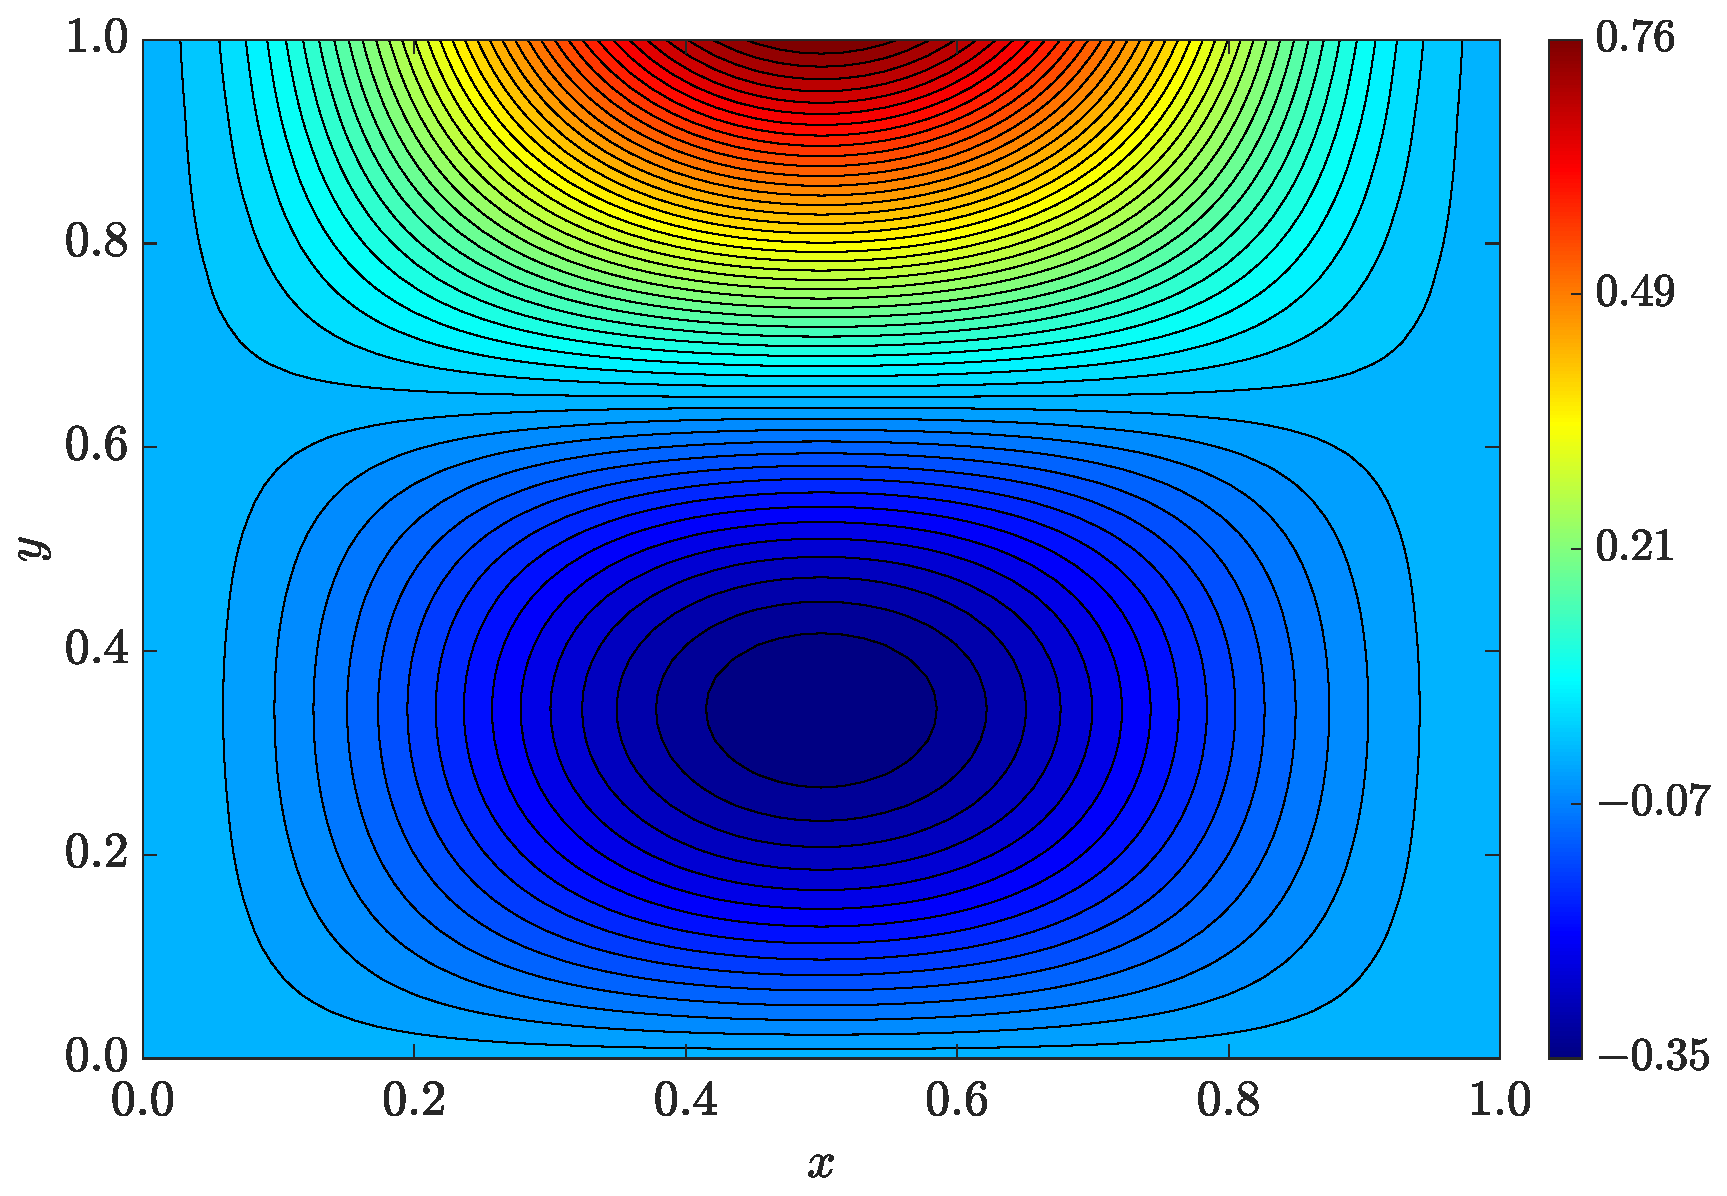
\includegraphics[width=\textwidth]{figures/Case12/UCM/Solutions/Exact_Map_NormErr_2nd_Betann_0.1_Re_1_Wi_1_epsilon_0_xi_0_alphaG_0_Dt_1e-06_at_0.05_tipsim_1_MMS_12_U.eps}
            \caption{$\overline{u}$}
            \label{fig_solexaustreamlineCase1}
        \end{subfigure}
        \vspace{0.2cm}
        \begin{subfigure}[b]{.47\textwidth}
            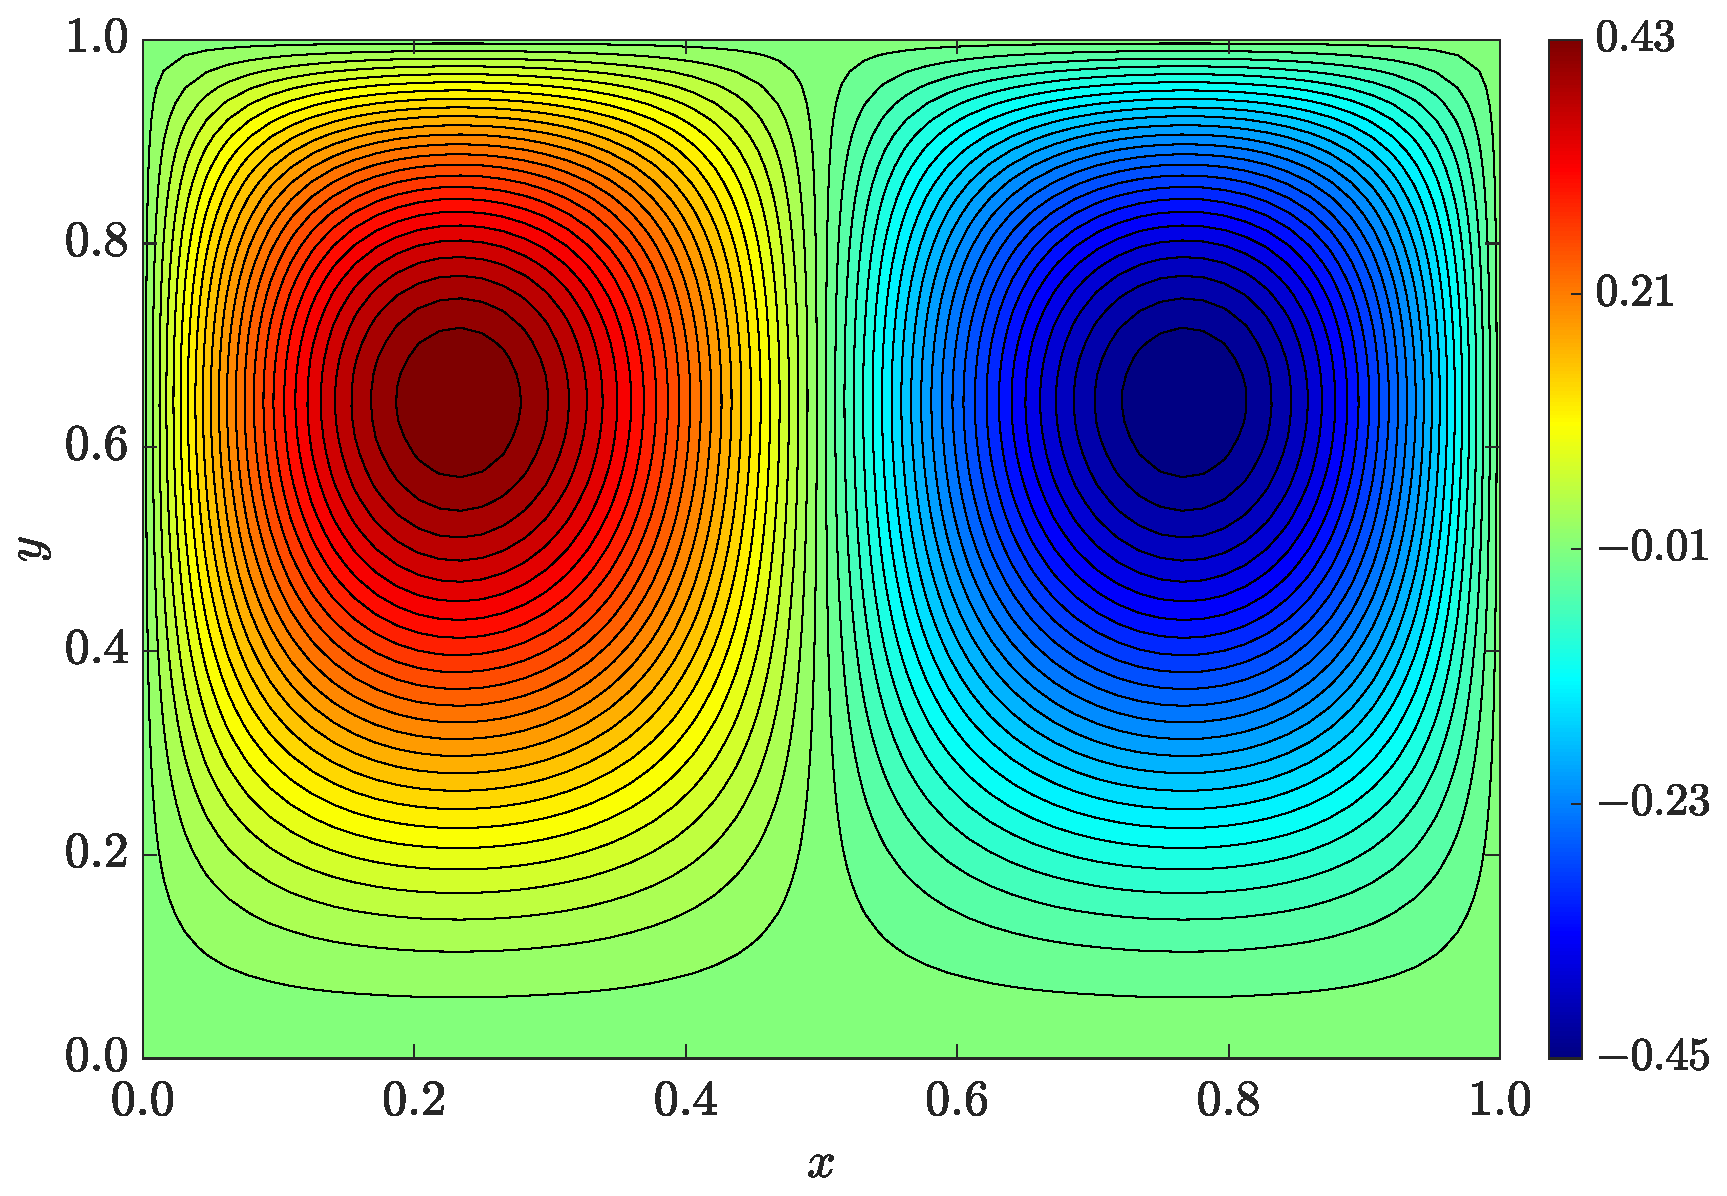
\includegraphics[width=\textwidth]{figures/Case12/UCM/Solutions/Exact_Map_NormErr_2nd_Betann_0.1_Re_1_Wi_1_epsilon_0_xi_0_alphaG_0_Dt_1e-06_at_0.05_tipsim_1_MMS_12_V.eps}
            \caption{$\widetilde{v}$}
            \label{fig_solexavstreamlineCase1}
        \end{subfigure}
        \begin{subfigure}[b]{.47\textwidth}
            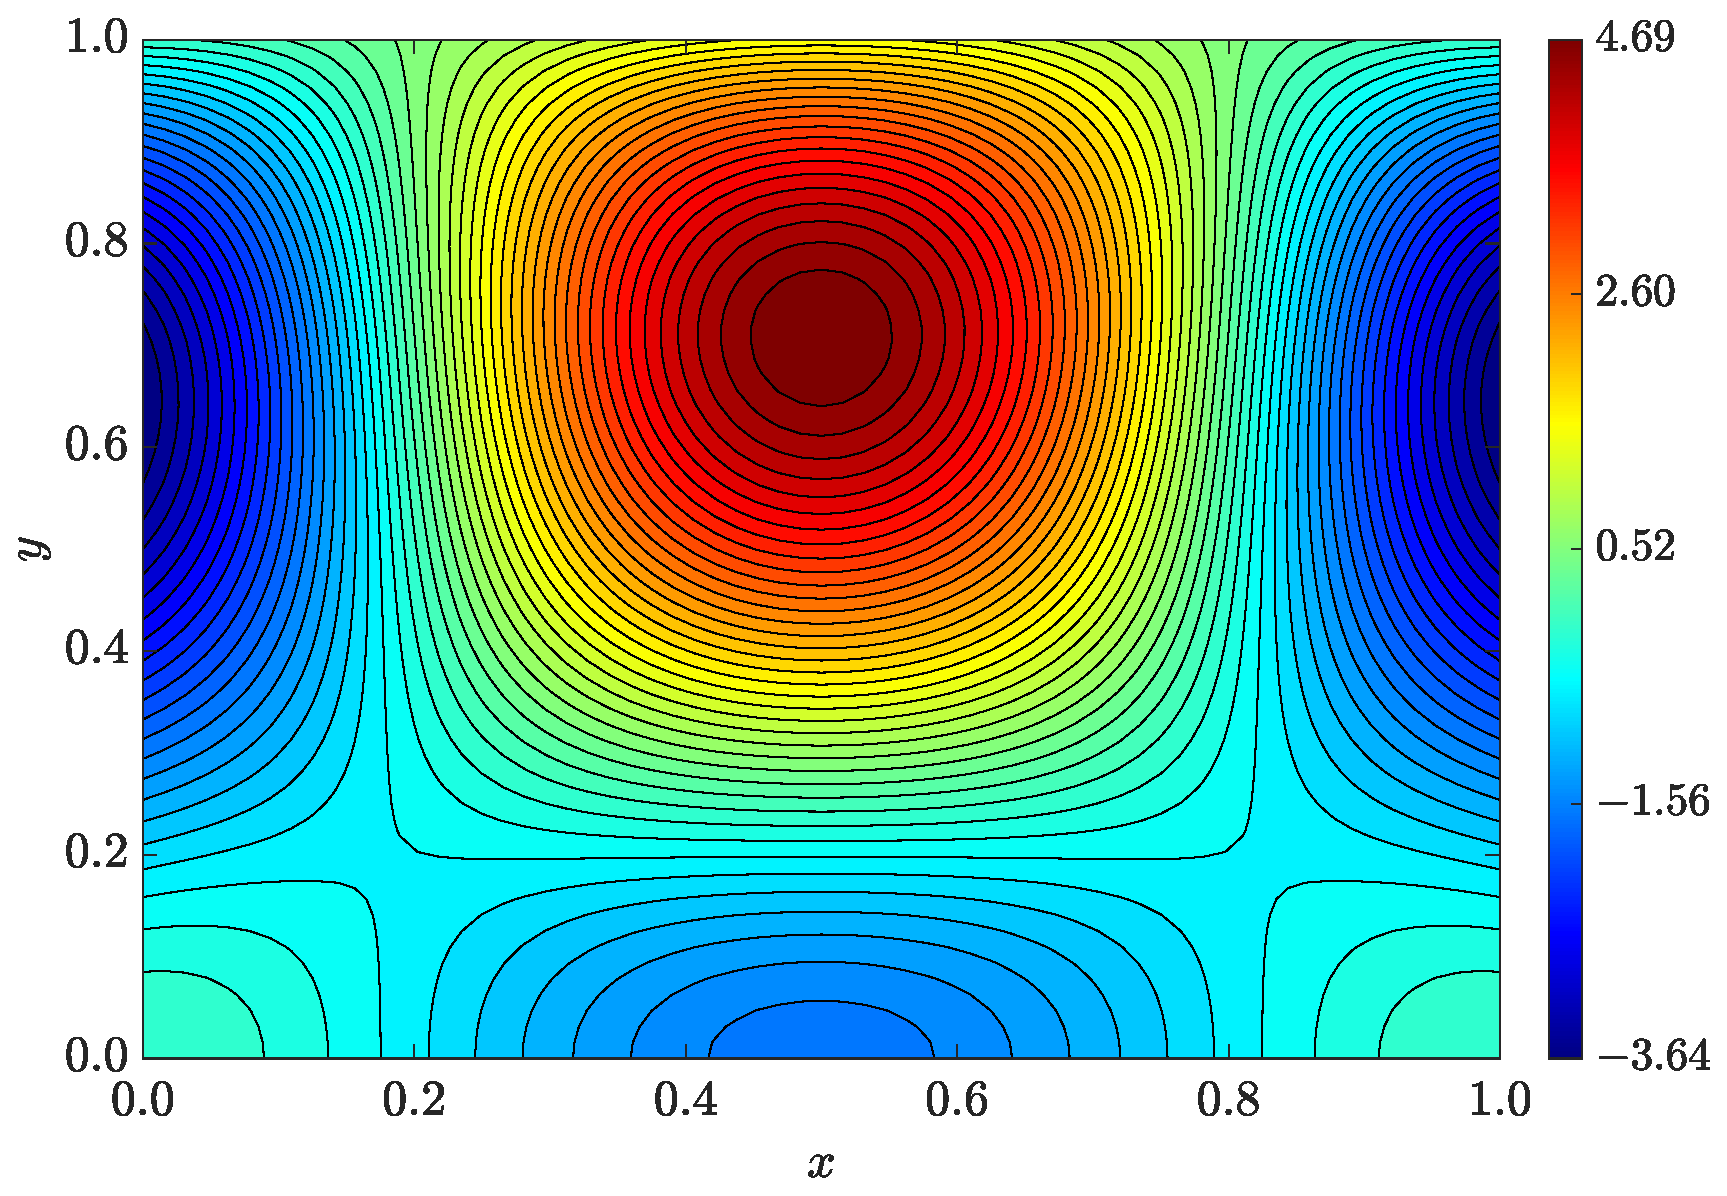
\includegraphics[width=\textwidth]{figures/Case12/UCM/Solutions/Exact_Map_NormErr_2nd_Betann_0.1_Re_1_Wi_1_epsilon_0_xi_0_alphaG_0_Dt_1e-06_at_0.05_tipsim_1_MMS_12_Wz.eps}
            \caption{$\widetilde{\omega_{z}}$}
            \label{fig_solexawzstreamlineCase1}
        \end{subfigure}
        \vspace{0.2cm}
        \begin{subfigure}[b]{.47\textwidth}
            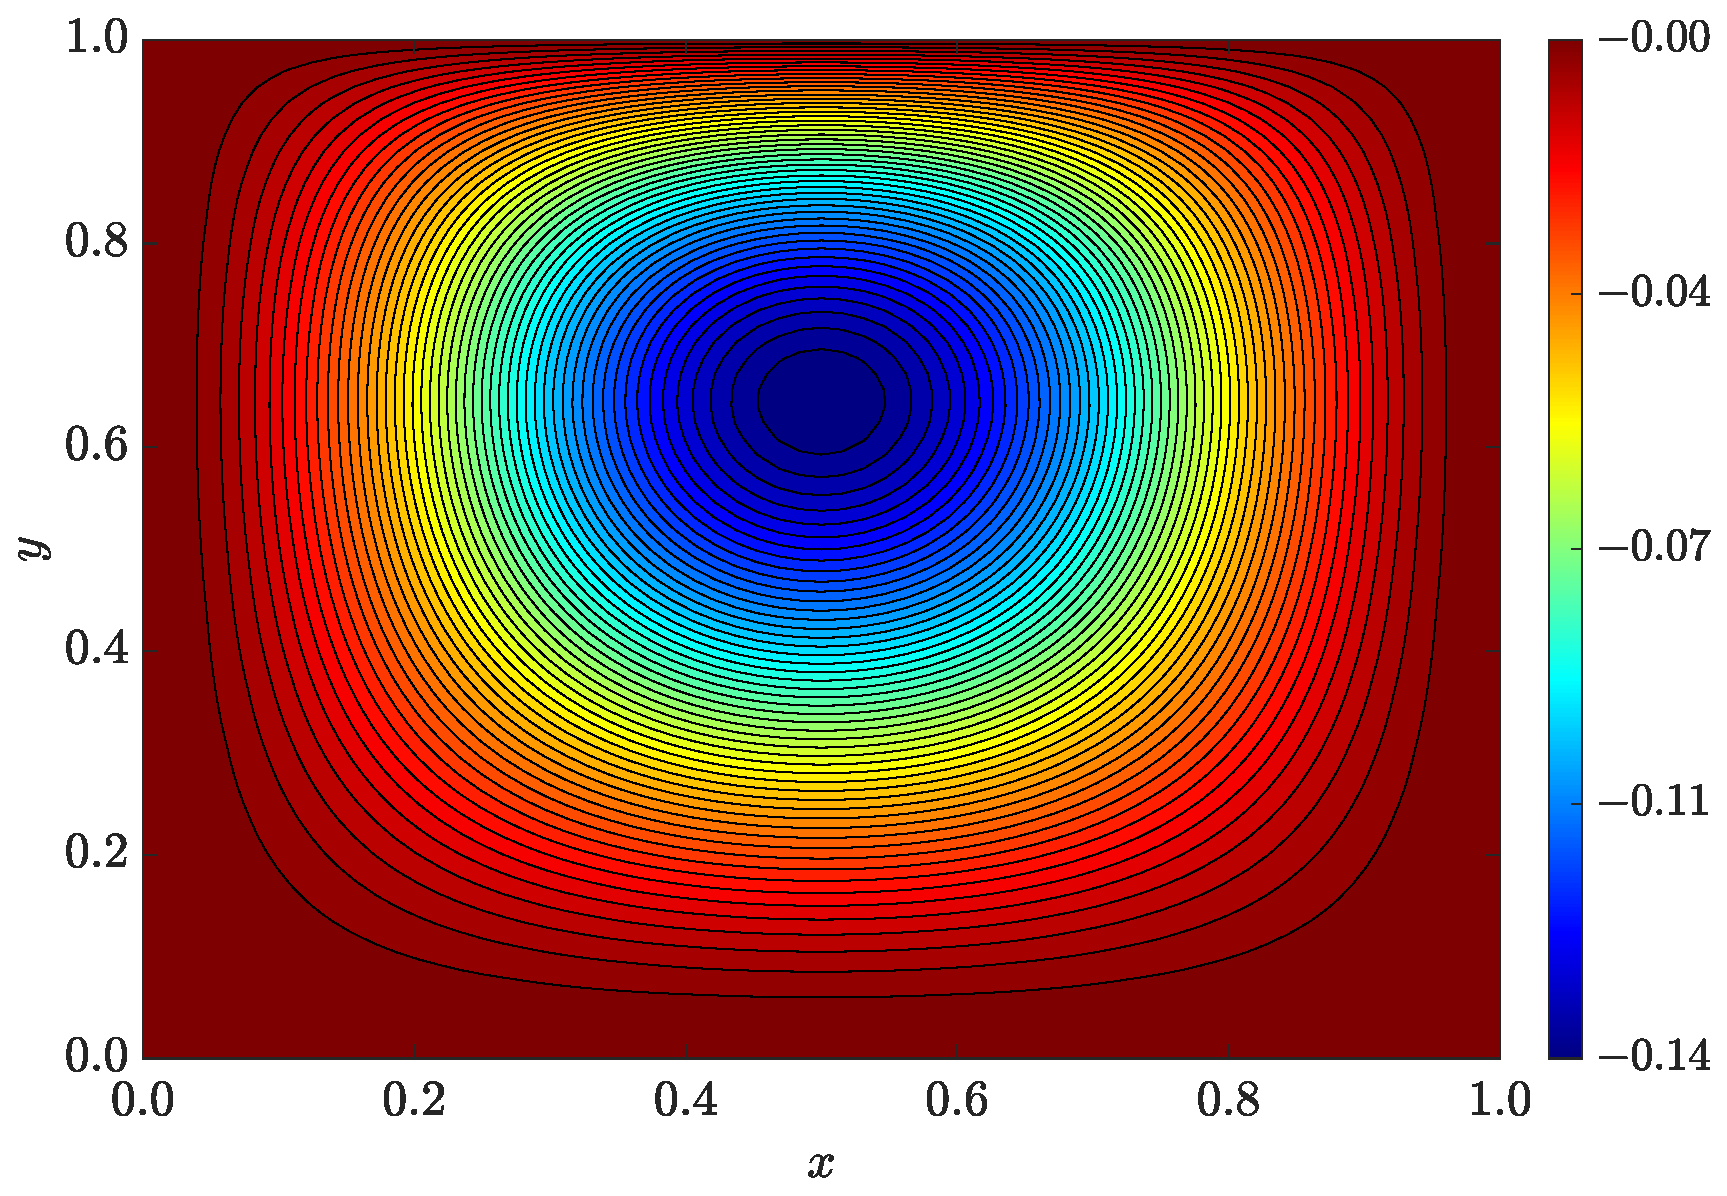
\includegraphics[width=\textwidth]{figures/Case12/UCM/Solutions/Exact_Map_NormErr_2nd_Betann_0.1_Re_1_Wi_1_epsilon_0_xi_0_alphaG_0_Dt_1e-06_at_0.05_tipsim_1_MMS_12_Psi.eps}
            \caption{$\widetilde{\psi}$}
            \label{fig_solexapsistreamlineCase1}
        \end{subfigure}
        \fdadospesquisa
\end{figure}

\begin{figure}[H]
        \centering
	\caption{Mapas de cores das soluções manufaturadas no regime de estado estacionário para os tensores, considerando $a = 0.05$ em $t = 0.1$}
        \label{fig_T_xxxyyy_sol_num_case1streamline2}
	\begin{subfigure}[b]{.47\textwidth}
            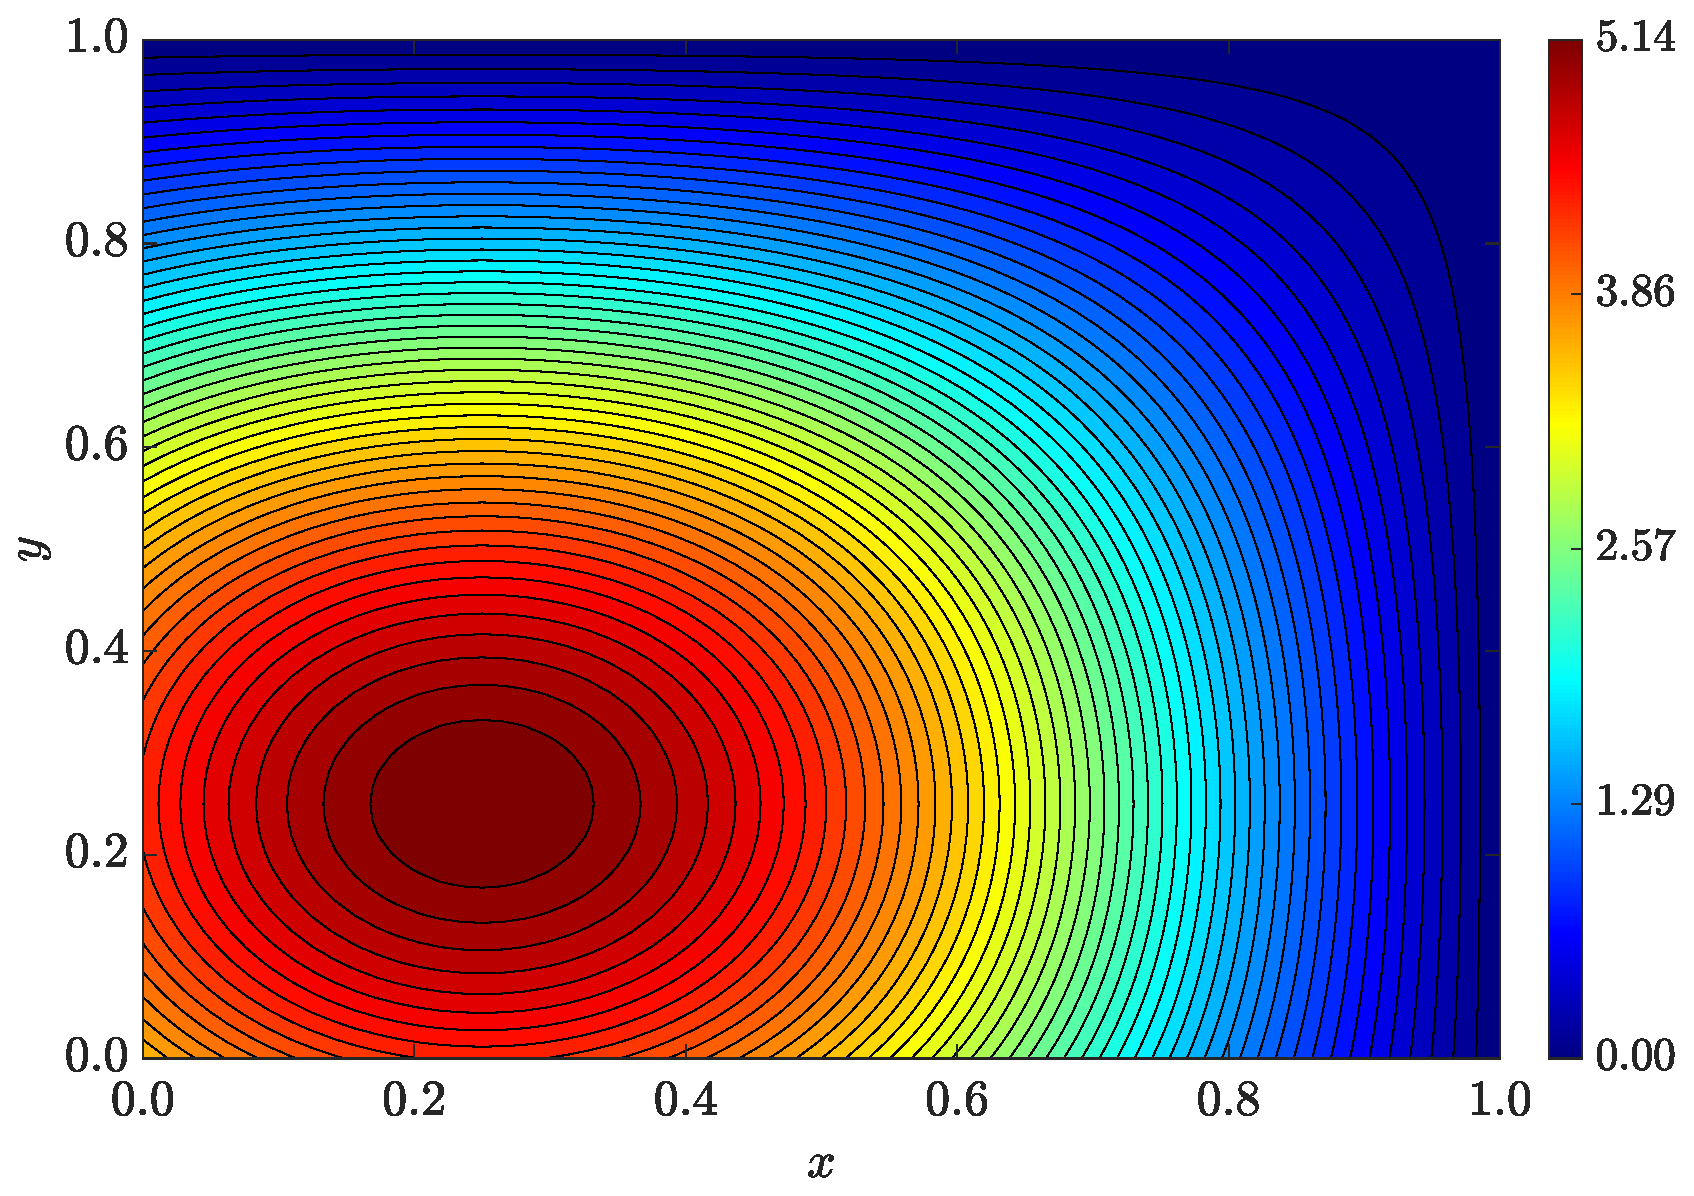
\includegraphics[width=\textwidth]{figures/Case12/UCM/Solutions/Exact_Map_NormErr_2nd_Betann_0.1_Re_1_Wi_1_epsilon_0_xi_0_alphaG_0_Dt_1e-06_at_0.05_tipsim_1_MMS_12_Txx.eps}
            \caption{$\overline{T}_{xx}$}
            \label{fig_solexatxxstreamlineCase1}
        \end{subfigure}
        \begin{subfigure}[b]{.47\textwidth}
            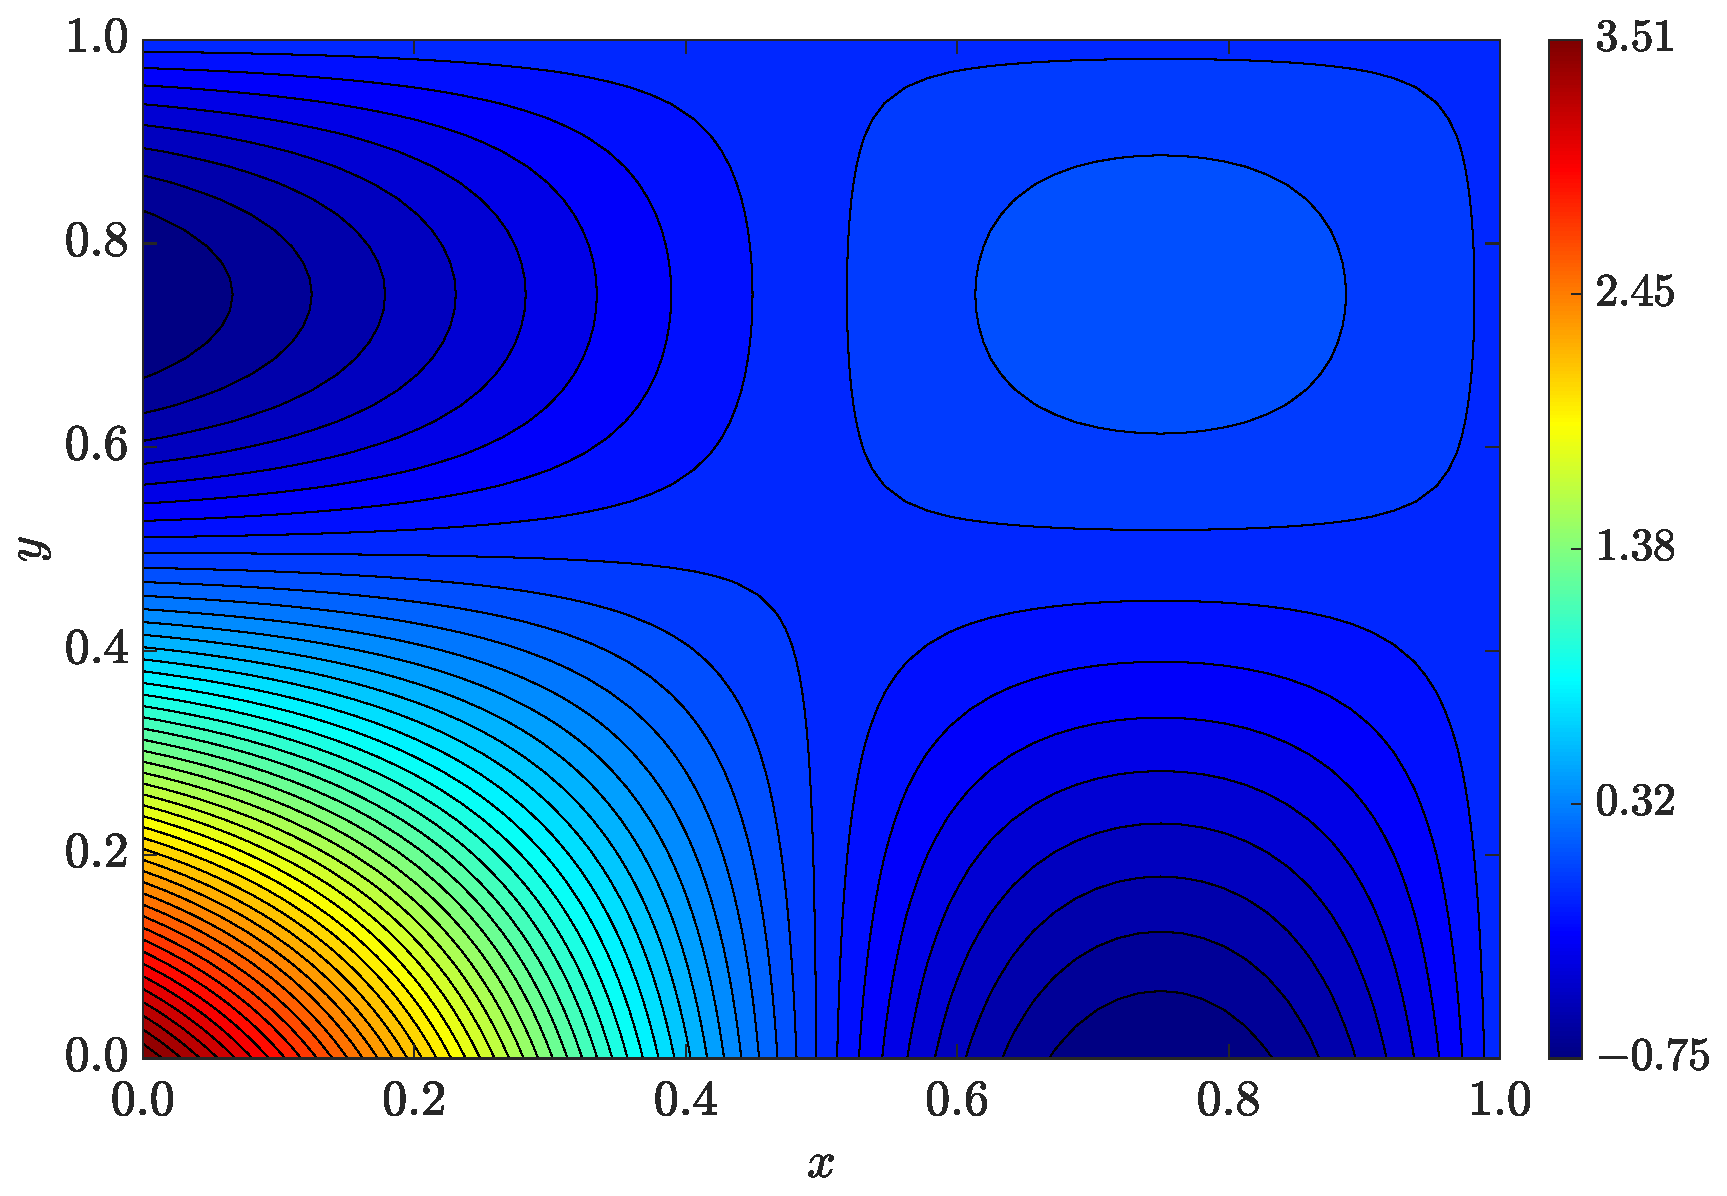
\includegraphics[width=\textwidth]{figures/Case12/UCM/Solutions/Exact_Map_NormErr_2nd_Betann_0.1_Re_1_Wi_1_epsilon_0_xi_0_alphaG_0_Dt_1e-06_at_0.05_tipsim_1_MMS_12_Txy.eps}
            \caption{$\overline{T}_{xy}$}
            \label{fig_solexatxystreamlineCase1}
        \end{subfigure}
        \vspace{0.2cm}
        \begin{subfigure}[b]{.47\textwidth}
            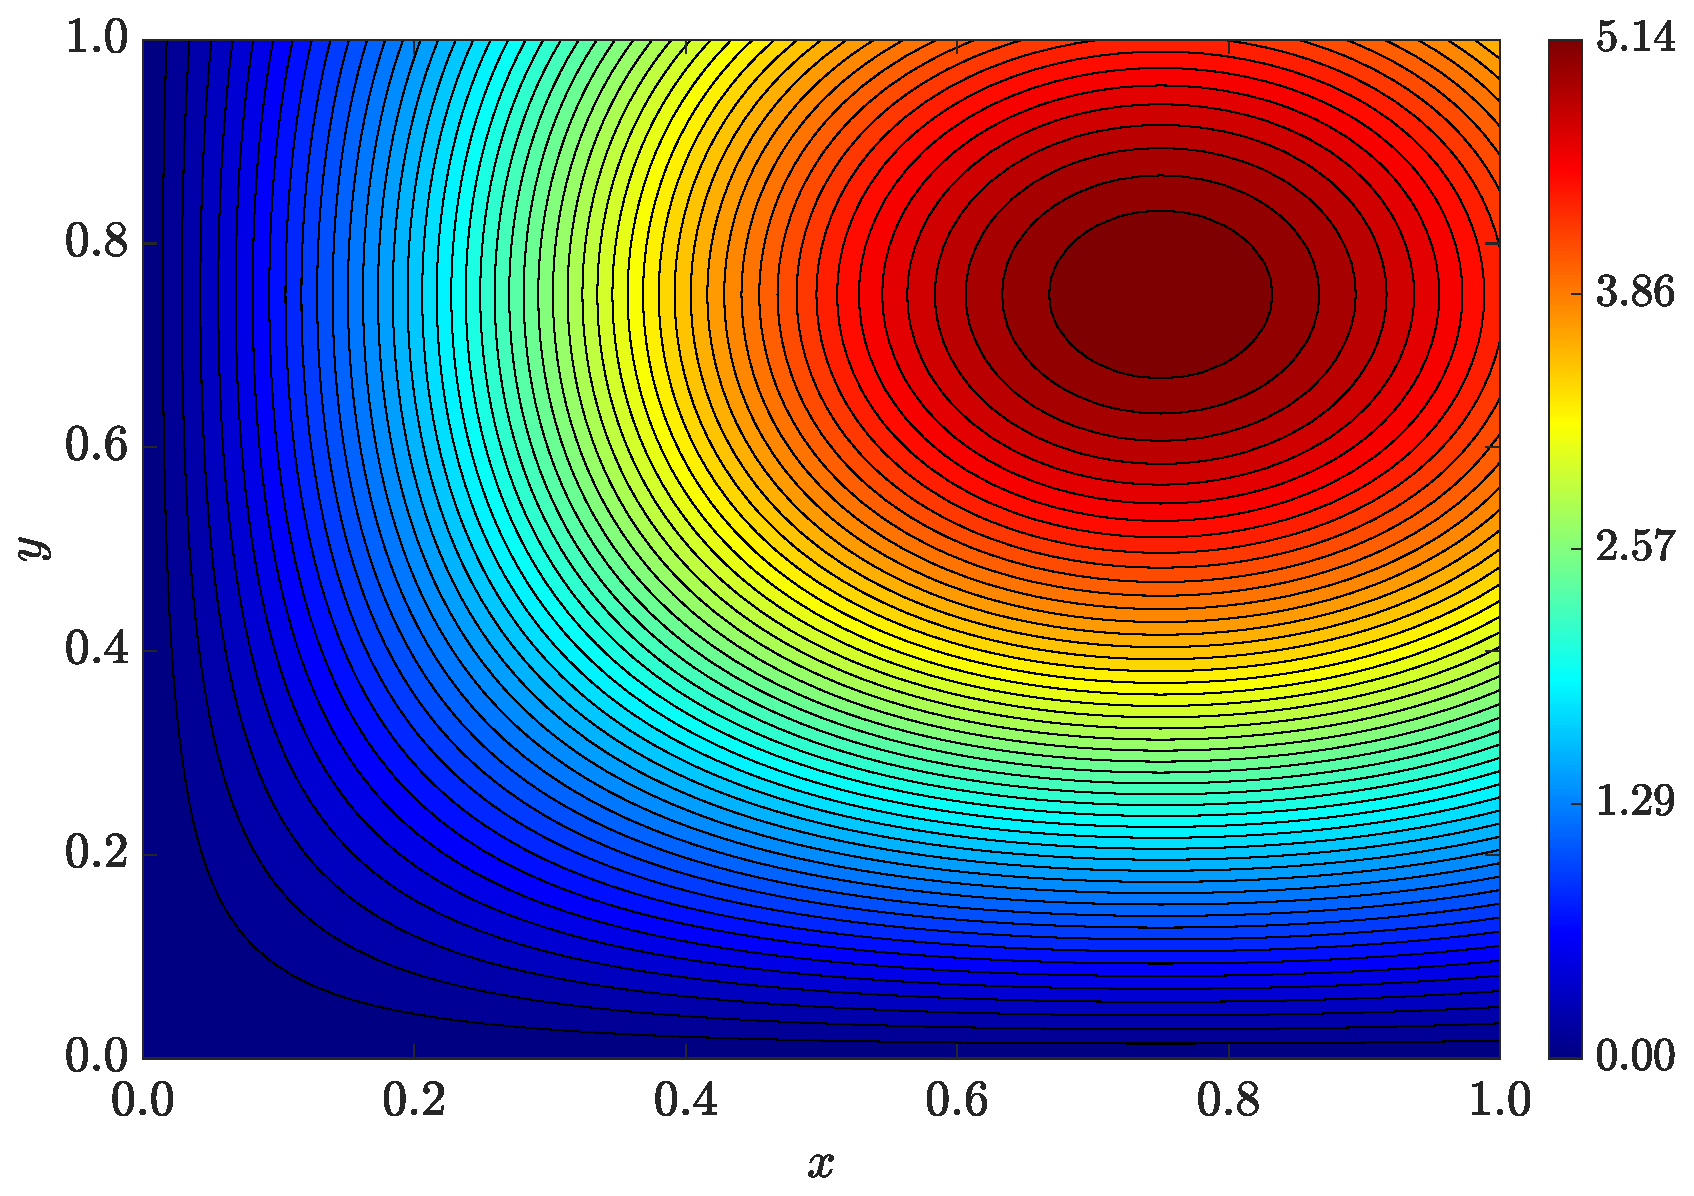
\includegraphics[width=\textwidth]{figures/Case12/UCM/Solutions/Exact_Map_NormErr_2nd_Betann_0.1_Re_1_Wi_1_epsilon_0_xi_0_alphaG_0_Dt_1e-06_at_0.05_tipsim_1_MMS_12_Tyy.eps}
            \caption{$\overline{T}_{yy}$}
            \label{fig_solexatyystreamlineCase1}
        \end{subfigure}
        \fdadospesquisa
\end{figure}

A partir deste ponto, será adotada uma convenção de notação para distinguir as soluções numéricas obtidas pelo código das soluções manufaturadas utilizadas como referência analítica. Todas as variáveis representadas por letras maiúsculas (por exemplo, $U$, $V$, $\Omega_z$, $\Psi$, $T_{xx}$, $T_{xy}$ e $T_{yy}$) correspondem às soluções numéricas computadas nas simulações. Por outro lado, as variáveis acompanhadas de til ($\widetilde{\cdot}$) ou barra superior ($\overline{\cdot}$) representam as soluções manufaturadas, derivadas simbolicamente e utilizadas para a verificação dos resultados. Essa distinção é utilizada para a interpretação dos gráficos, tabelas e análises de erro apresentadas nas próximas seções.

\subsection{Caso de verificação usando o modelo UCM}

As simulações numéricas realizadas para verificar o código de alta ordem desenvolvido para escoamentos de fluidos viscoelásticos foram configuradas utilizando o modelo UCM, com números de Reynolds variando entre $Re = 1,\ 10,\ 100,\ 400$ e $1000$, número de Weissenberg $Wi = 1,\ 5$ e $10$. Para este modelo, a razão de viscosidade do solvente foi fixada em $\beta_{nn} = 0$, representando o comportamento puramente viscoelástico sem influência da viscosidade do solvente, com o objetivo de avaliar o desempenho do modelo em diferentes regimes de escoamento viscoelástico.

Dado que os resultados obtidos para as diferentes combinações de parâmetros apresentaram comportamentos qualitativamente semelhantes, assim apresenta-se detalhadamente apenas um dos casos simulados. Essa escolha visa evitar repetições e tornar a análise mais objetiva, sem prejuízo à generalidade das conclusões sobre a acurácia e estabilidade do método numérico proposto. A \autoref{UCMerror1} apresenta os gráficos de erro para os componentes do campo de velocidade, vorticidade e função de corrente, enquanto a \autoref{UCMerror2} complementa essa análise mostrando os erros associados aos tensores no escoamento de fluido viscoelástico UCM. Esses gráficos mostram a evolução dos erros para $Re = 100$, $Wi = 1$ e $\beta_{nn} = 0$. Observou-se que, à medida que a malha é refinada, os erros diminuem consideravelmente, confirmando a eficácia do esquema numérico na captura das propriedades do escoamento.
\begin{figure}[H]
        \centering
	\caption{Erro para o campo de velocidades $(\overline{u},\tilde{v})$, vorticidade $(\tilde{\omega_{z}})$ e função de corrente $(\tilde{\psi})$, utilizando $Re=100$, $\beta_{nn} = 0$ e $Wi=1$ para o escoamento de fluido viscoelástico como o modelo UCM}
        \label{UCMerror1}
	\begin{subfigure}[b]{.47\textwidth}
            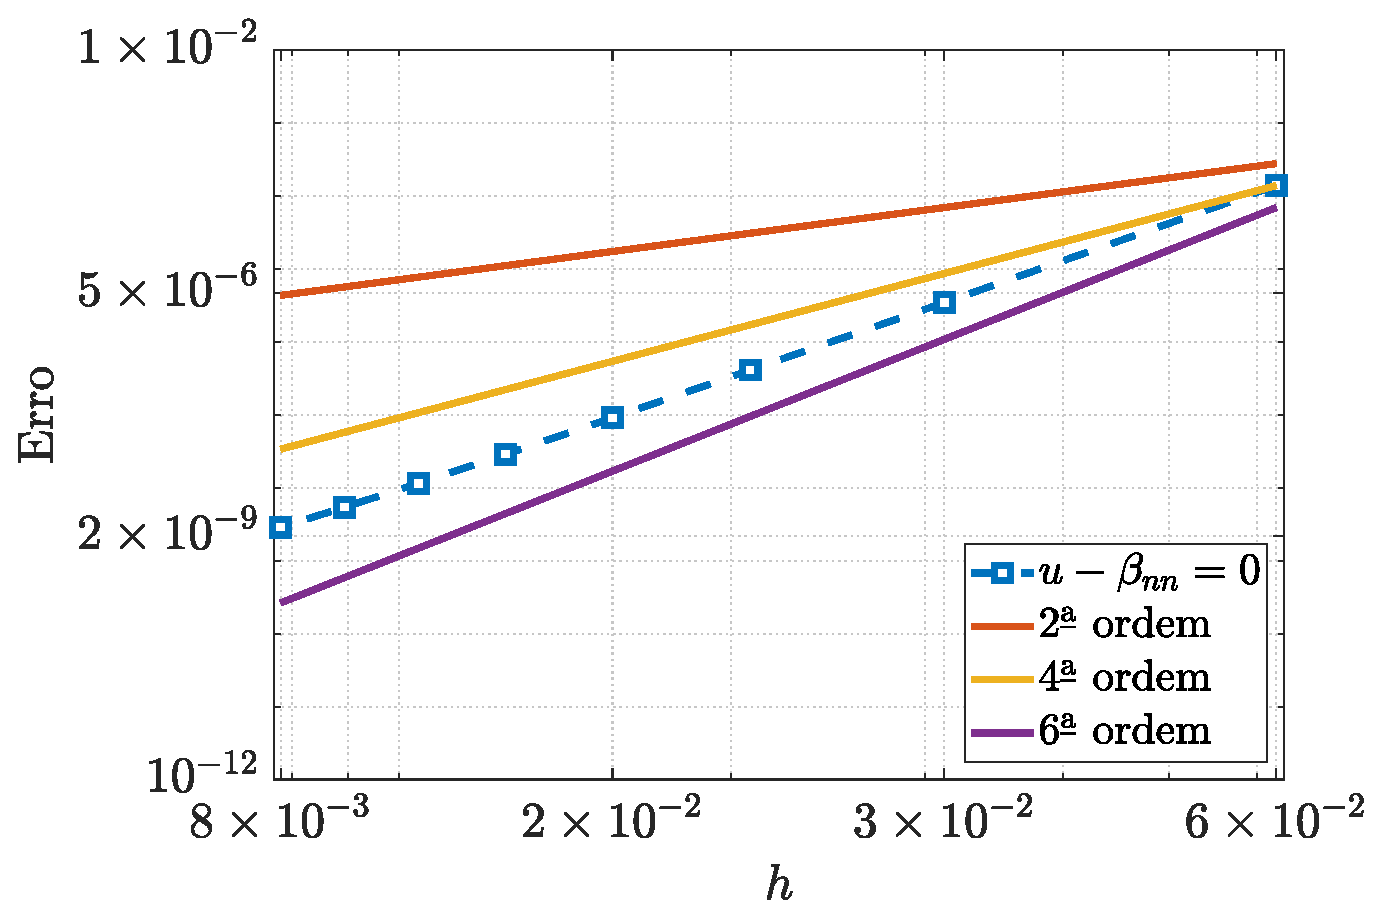
\includegraphics[width=\textwidth]{figures/Case12/UCM/Errors/NormErr_2nd_Re_100_Wi_1_epsilon_0_xi_0_alphaG_0_Dt_1e-06_at_0.05_tipsim_1_MMS_12_U.eps}
            \caption{$||U - \overline{u}||_{2}$}
            \label{error_u_2nd_Case1_ucm}
        \end{subfigure}
        \vspace{0.2cm}
        \qquad
        \begin{subfigure}[b]{.47\textwidth}
            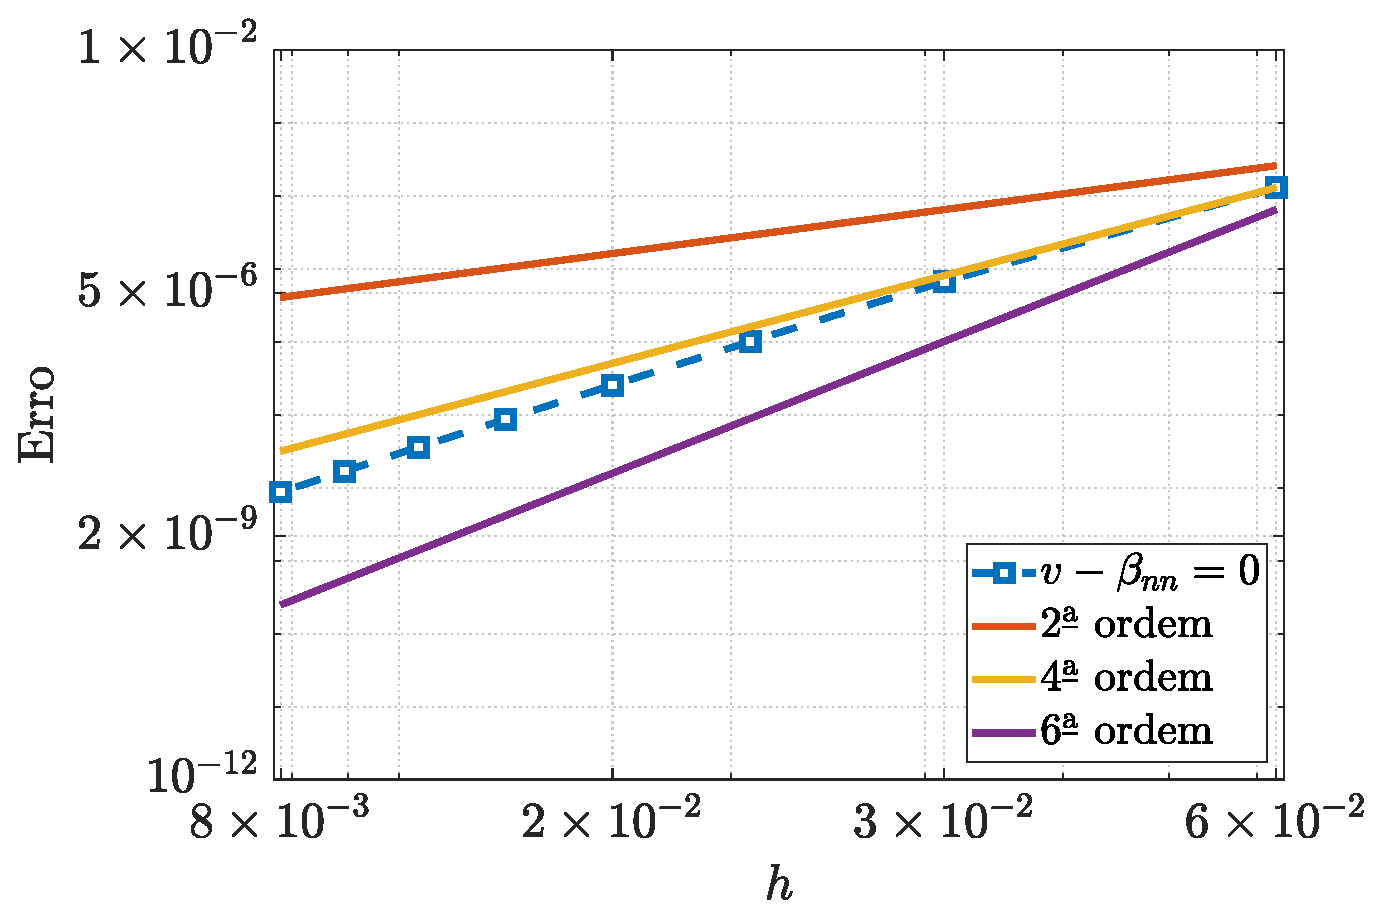
\includegraphics[width=\textwidth]{figures/Case12/UCM/Errors/NormErr_2nd_Re_100_Wi_1_epsilon_0_xi_0_alphaG_0_Dt_1e-06_at_0.05_tipsim_1_MMS_12_V.eps}
            \caption{$||V - \widetilde{v}||_{2}$}
            \label{error_v_2nd_Case1_ucm}
        \end{subfigure}
        \qquad
        \begin{subfigure}[b]{.47\textwidth}
            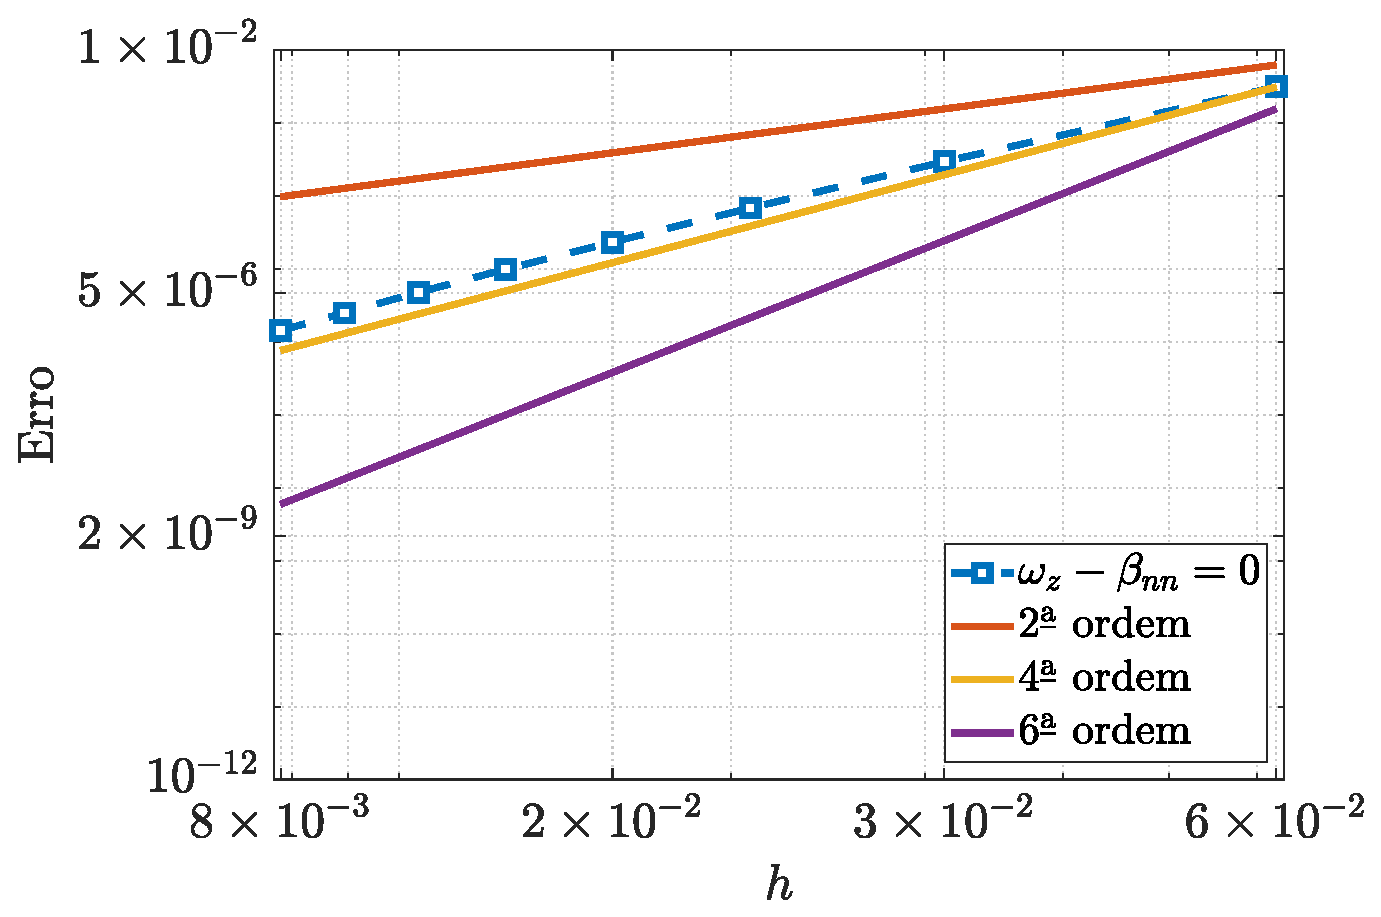
\includegraphics[width=\textwidth]{figures/Case12/UCM/Errors/NormErr_2nd_Re_100_Wi_1_epsilon_0_xi_0_alphaG_0_Dt_1e-06_at_0.05_tipsim_1_MMS_12_Wz.eps}
            \caption{$||\Omega_{z} - \widetilde{\omega_{z}}||_{2}$}
            \label{error_wz_2nd_Case1_ucm}
        \end{subfigure}
        \vspace{0.02cm}
        \qquad
        \begin{subfigure}[b]{.47\textwidth}
            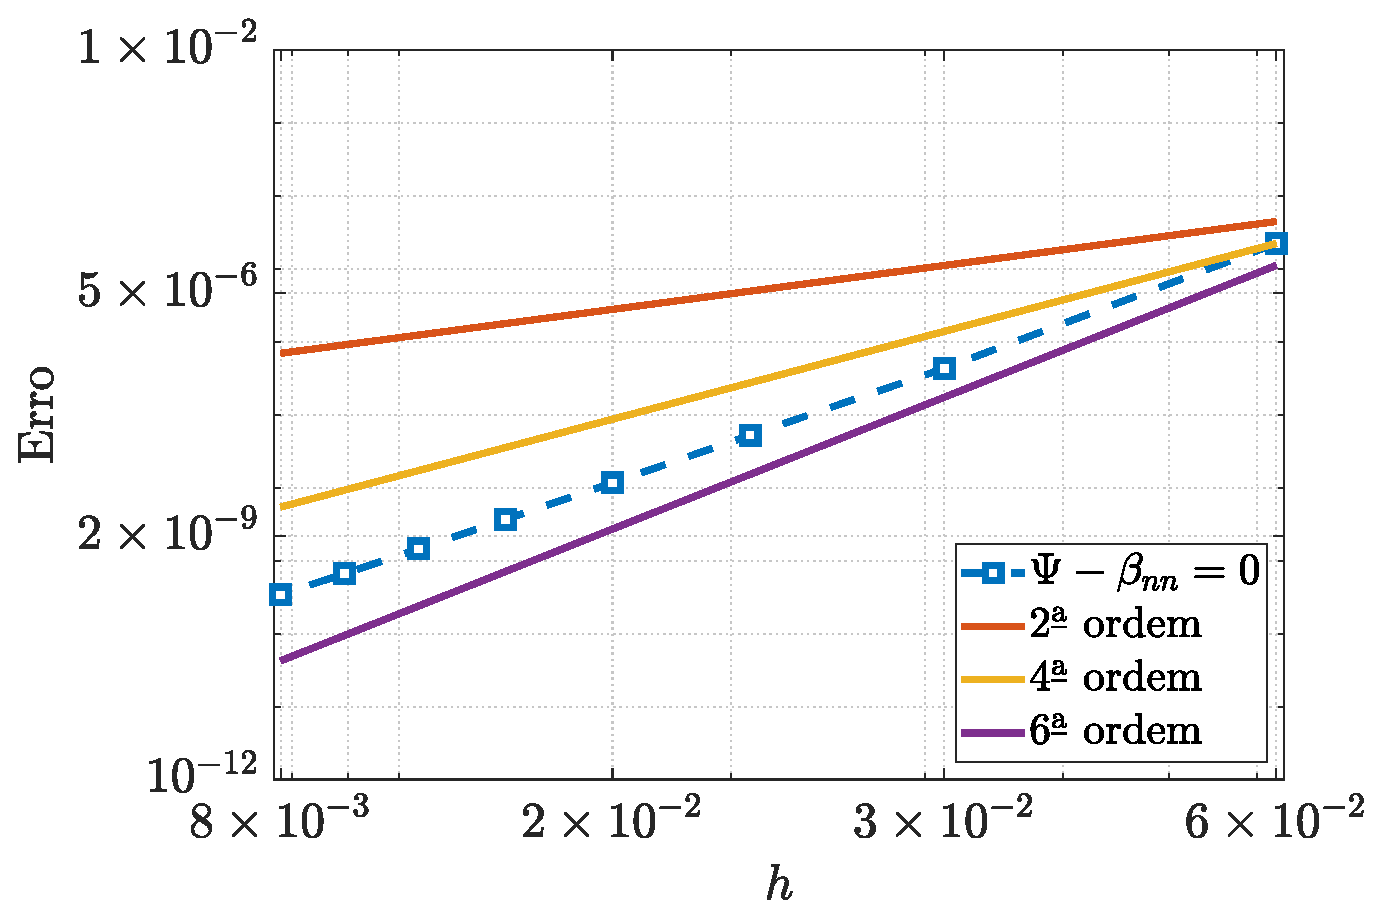
\includegraphics[width=\textwidth]{figures/Case12/UCM/Errors/NormErr_2nd_Re_100_Wi_1_epsilon_0_xi_0_alphaG_0_Dt_1e-06_at_0.05_tipsim_1_MMS_12_Psi.eps}
            \caption{$||\Psi - \widetilde{\Psi}||_{2}$}
            \label{error_psi_2nd_Case1_ucm}
        \end{subfigure}
        \fdadospesquisa
\end{figure}

\begin{figure}[H]
    \centering
    \caption{Erro para as componentes dos tensores de tensões, utilizando $Re=100$, $\beta_{nn} = 0$ e $Wi=1$ para o escoamento de fluido viscoelástico como o modelo UCM}
    \label{UCMerror2}
    \begin{subfigure}[b]{.47\textwidth}
        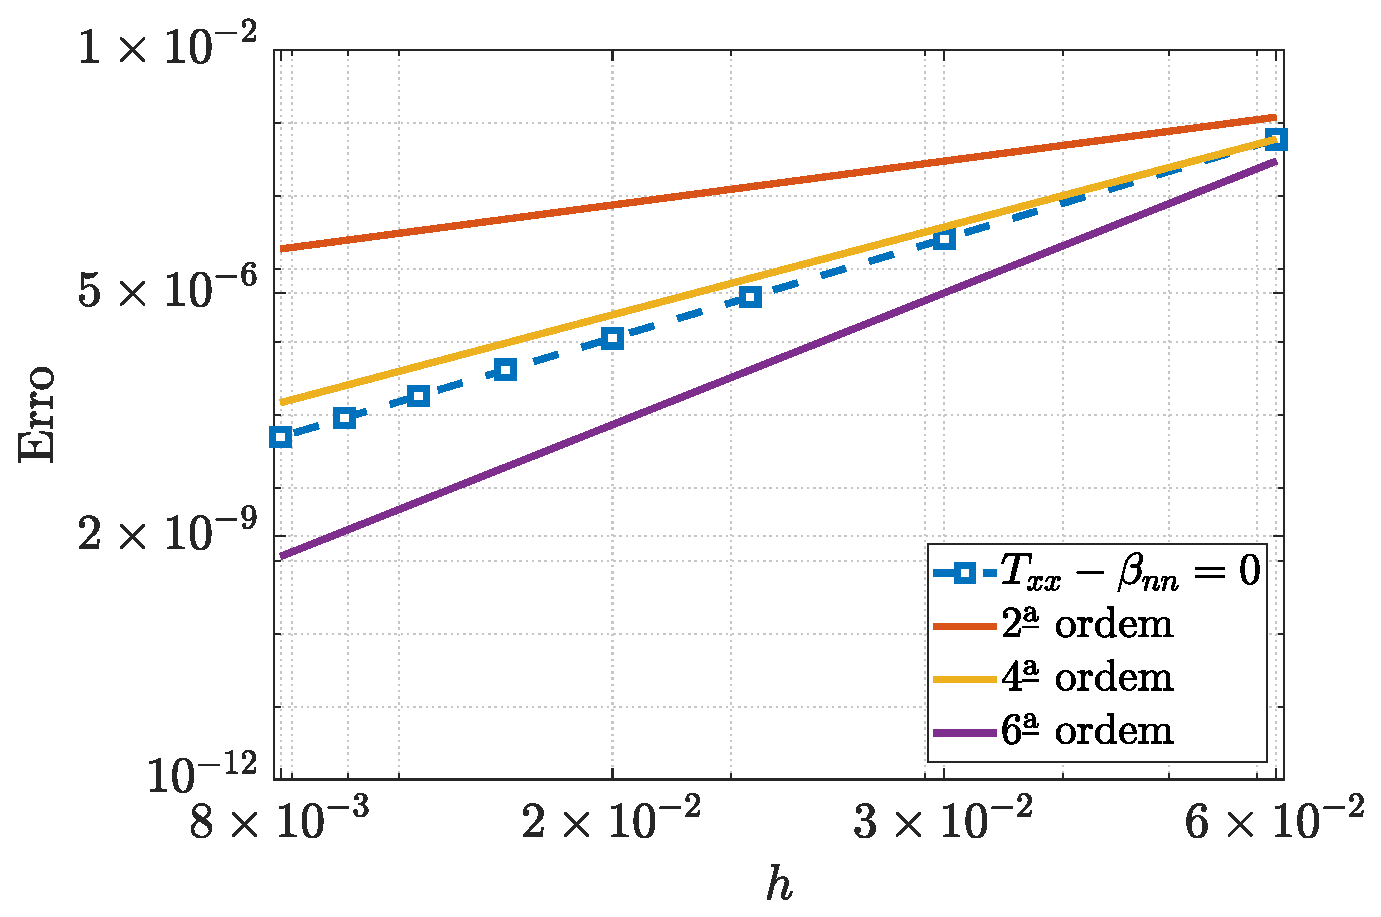
\includegraphics[width=\textwidth]{figures/Case12/UCM/Errors/NormErr_2nd_Re_100_Wi_1_epsilon_0_xi_0_alphaG_0_Dt_1e-06_at_0.05_tipsim_1_MMS_12_Txx.eps}
        \caption{$||T_{xx} - \overline{T}_{xx}||_{2}$}
        \label{error_txx_2nd_Case1_ucm}
    \end{subfigure}
    \vspace{0.2cm}
    \qquad
    \begin{subfigure}[b]{.47\textwidth}
        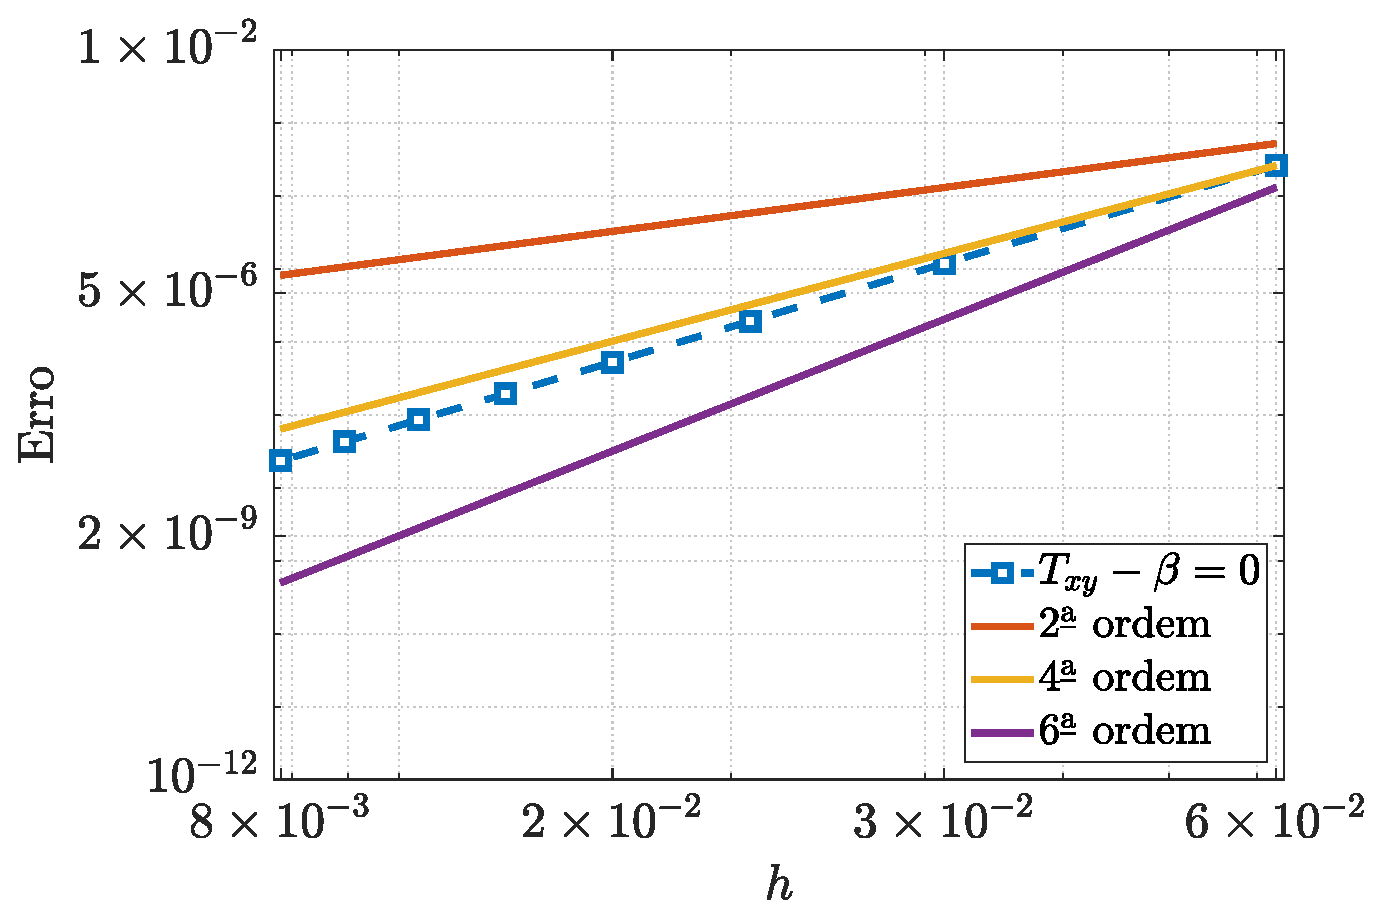
\includegraphics[width=\textwidth]{figures/Case12/UCM/Errors/NormErr_2nd_Re_100_Wi_1_epsilon_0_xi_0_alphaG_0_Dt_1e-06_at_0.05_tipsim_1_MMS_12_Txy.eps}
        \caption{$||T_{xy} - \overline{T}_{xy}||_{2}$}
        \label{error_txy_2nd_Case1_ucm}
    \end{subfigure}
    \qquad
    \begin{subfigure}[b]{.47\textwidth}
        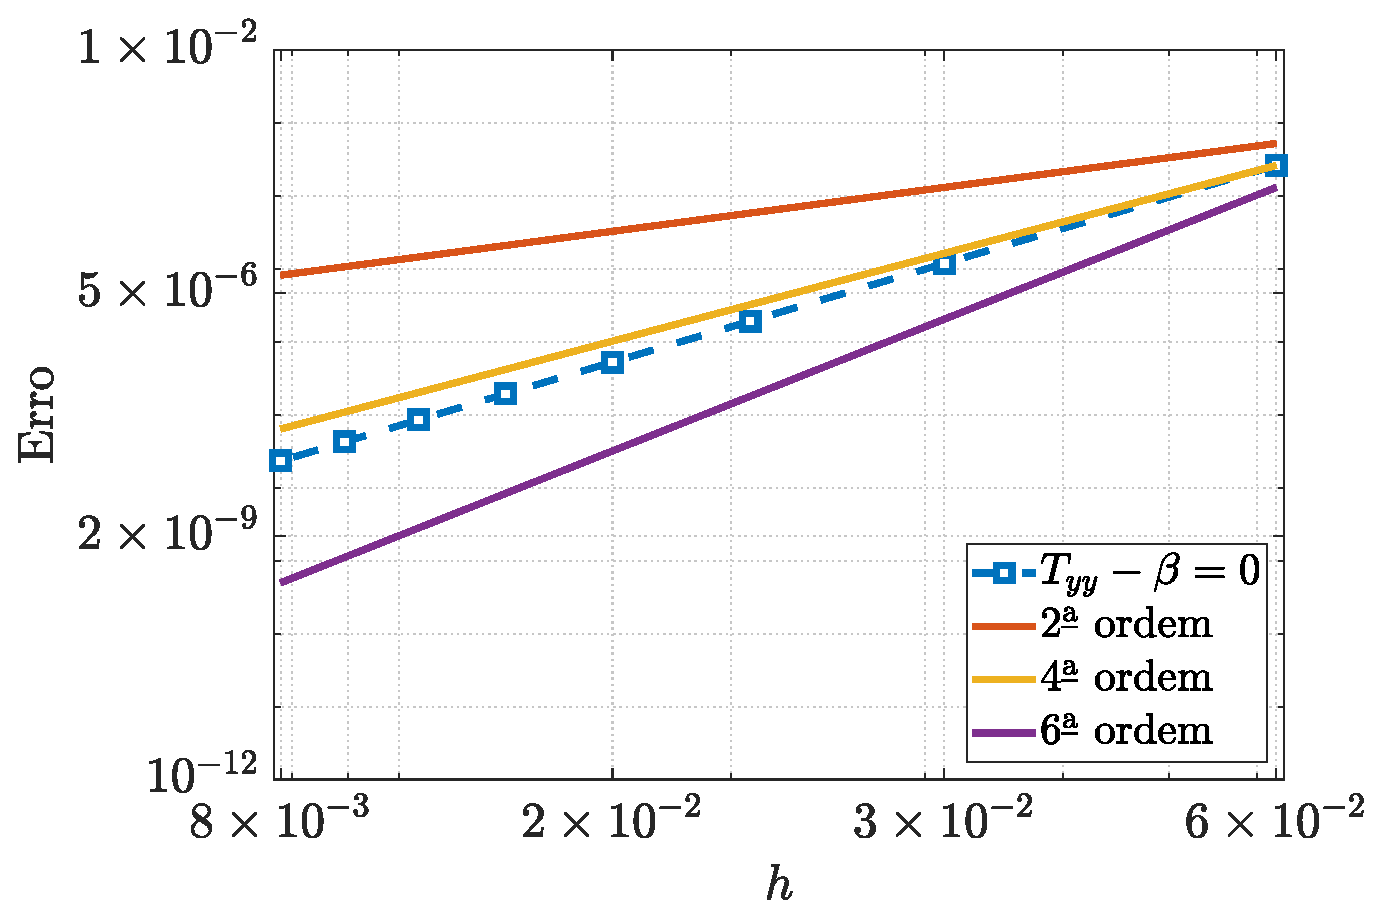
\includegraphics[width=\textwidth]{figures/Case12/UCM/Errors/NormErr_2nd_Re_100_Wi_1_epsilon_0_xi_0_alphaG_0_Dt_1e-06_at_0.05_tipsim_1_MMS_12_Tyy.eps}
        \caption{$||T_{yy} - \overline{T}_{yy}||_{2}$}
        \label{error_tyy_2nd_Case1_ucm}
    \end{subfigure}
    \fdadospesquisa
\end{figure}

As \autoref{UCMerror1} e a \autoref{UCMerror2} ilustram a ordem teórica de convergência obtida pelo código desenvolvido. Para proporcionar uma visão mais clara da convergência da vorticidade, a \autoref{tab_UCMWzResumida} apresenta os cálculos correspondentes para $Re = 1,$ $100,$ $400$ e $1000$, onde o comportamento discutido anteriormente pode ser claramente observado.
\begin{table}[H]
	\IBGEtab{
            \caption{Erros numéricos e cálculo da ordem de convergência para a vorticidade $(\omega_{z})$, utilizando o parâmetro $Wi=1$, para o escoamento de fluido viscoelástico UCM}
            \label{tab_UCMWzResumida}
		}{
            \begin{tabular*}{\textwidth}{@{\extracolsep\fill}c|c|cc|cc@{}}
                \toprule
                 \multirow{2}{*}{$Re$} & \multirow{2}{*}{Malha} & \multicolumn{2}{c}{$\beta_{nn}=0$ - $\omega_{z}$} & \multicolumn{2}{c}{$\beta_{nn}=0$ - $T_{xx}$} \\ \cline{3-6}
                     & & Erro & p & Erro & p \\ \midrule
                    \multirow{7}{*}{1.00} & $17\times 17$ & 3.10e-03 & --- & 5.97e-04 & ---\\
                    & $33\times 33$ & 2.93e-04 & 3.40 & 2.56e-05 & 4.54\\
                    & $49\times 49$ & 6.78e-05 & 3.61 & 4.10e-06 & 4.52\\
                    & $65\times 65$ & 2.31e-05 & 3.74 & 1.12e-06 & 4.51\\
                    & $81\times 81$ & 9.80e-06 & 3.85 & 4.10e-07 & 4.50\\
                    & $97\times 97$ & 4.72e-06 & 4.01 & 1.80e-07 & 4.50\\
                    & $113\times 113$ & 2.46e-06 & 4.22 & 9.02e-08 & 4.50\\
                    & $129\times 129$ & 1.41e-06 & 4.16 & 4.94e-08 & 4.50\\
                    \midrule
                    \multirow{7}{*}{100.00} & $17\times 17$ & 3.10e-03 & --- & 5.97e-04 & ---\\
                    & $33\times 33$ & 2.93e-04 & 3.40 & 2.56e-05 & 4.54\\
                    & $49\times 49$ & 6.78e-05 & 3.61 & 4.10e-06 & 4.52\\
                    & $65\times 65$ & 2.32e-05 & 3.74 & 1.12e-06 & 4.51\\
                    & $81\times 81$ & 9.83e-06 & 3.84 & 4.10e-07 & 4.50\\
                    & $97\times 97$ & 4.74e-06 & 4.00 & 1.80e-07 & 4.50\\
                    & $113\times 113$ & 2.48e-06 & 4.21 & 9.02e-08 & 4.50\\
                    & $129\times 129$ & 1.42e-06 & 4.16 & 4.94e-08 & 4.50\\
                    \midrule
                    \multirow{7}{*}{400.00} & $17\times 17$ & 3.10e-03 & --- & 5.97e-04 & ---\\
                    & $33\times 33$ & 2.93e-04 & 3.40 & 2.56e-05 & 4.54\\
                    & $49\times 49$ & 6.78e-05 & 3.61 & 4.10e-06 & 4.52\\
                    & $65\times 65$ & 2.32e-05 & 3.74 & 1.12e-06 & 4.51\\
                    & $81\times 81$ & 9.83e-06 & 3.84 & 4.10e-07 & 4.50\\
                    & $97\times 97$ & 4.74e-06 & 4.00 & 1.80e-07 & 4.50\\
                    & $113\times 113$ & 2.48e-06 & 4.21 & 9.02e-08 & 4.50\\
                    & $129\times 129$ & 1.42e-06 & 4.16 & 4.94e-08 & 4.50\\
                    \midrule
                    \multirow{7}{*}{1000.00} & $17\times 17$ & 3.10e-03 & --- & 5.97e-04 & ---\\
                    & $33\times 33$ & 2.93e-04 & 3.40 & 2.56e-05 & 4.54\\
                    & $49\times 49$ & 6.78e-05 & 3.61 & 4.10e-06 & 4.52\\
                    & $65\times 65$ & 2.32e-05 & 3.74 & 1.12e-06 & 4.51\\
                    & $81\times 81$ & 9.83e-06 & 3.84 & 4.10e-07 & 4.50\\
                    & $97\times 97$ & 4.74e-06 & 4.00 & 1.80e-07 & 4.50\\
                    & $113\times 113$ & 2.48e-06 & 4.21 & 9.02e-08 & 4.50\\
                    & $129\times 129$ & 1.42e-06 & 4.16 & 4.94e-08 & 4.50\\
                    \bottomrule
                \end{tabular*}
		}{
		\fdadospesquisa
	}
\end{table}

\subsection{Caso de verificação usando o modelo Oldroyd-B}

As simulações numéricas realizadas para verificar o código de alta ordem desenvolvido para escoamentos de fluidos viscoelásticos foram configuradas utilizando o modelo Oldroyd-B, com números de Reynolds variando entre $Re = 1,\ 10,\ 100,\ 400,$ e $1000$, número de Weissenberg $Wi = 1,\ 5$ e $10$. Além disso, a razão de viscosidade do solvente foi definida como $\beta_{nn} = 0.1,\ 0.5,\ 0.9$ e $1$, com o objetivo de avaliar o desempenho do modelo em diferentes regimes de escoamento. Um valor elevado de $\beta_{nn} = 1$ representa o comportamento de um fluido Newtoniano, enquanto valores mais baixos indicam um comportamento progressivamente mais viscoelástico.

A \autoref{OBerror1} apresenta os gráficos de erro para os componentes do campo de velocidade, vorticidade e função de corrente, enquanto a \autoref{OBerror2} complementa essa análise mostrando os erros associados aos tensores de tensão extra no escoamento de fluido viscoelástico Oldroyd-B. Esses gráficos mostram a evolução dos erros para $Re = 100$, $Wi = 1$, e $\beta_{nn} = 0.1,\ 0.5$ e $0.9$. Vale destacar que os resultados para $\beta_{nn} = 1.0$ foram omitidos, pois os erros correspondentes estavam na ordem de $10^{-18}$, o que teria distorcido a visualização comparativa dos outros valores de $\beta_{nn}$. Finalmente, a \autoref{tab_OldroydBTxxResumida} resume a ordem de convergência e os erros calculados nas malhas consideradas.
\begin{figure}[H]
        \centering
	\caption{Erro para o campo de velocidades $(\overline{u},\tilde{v})$, vorticidade $(\tilde{\omega_{z}})$ e função de corrente $(\tilde{\psi})$, considerando $Re=100$ e $Wi=1$ para o escoamento de fluido viscoelástico como o modelo Oldroyd-B}
        \label{OBerror1}
	\begin{subfigure}[b]{.47\textwidth}
            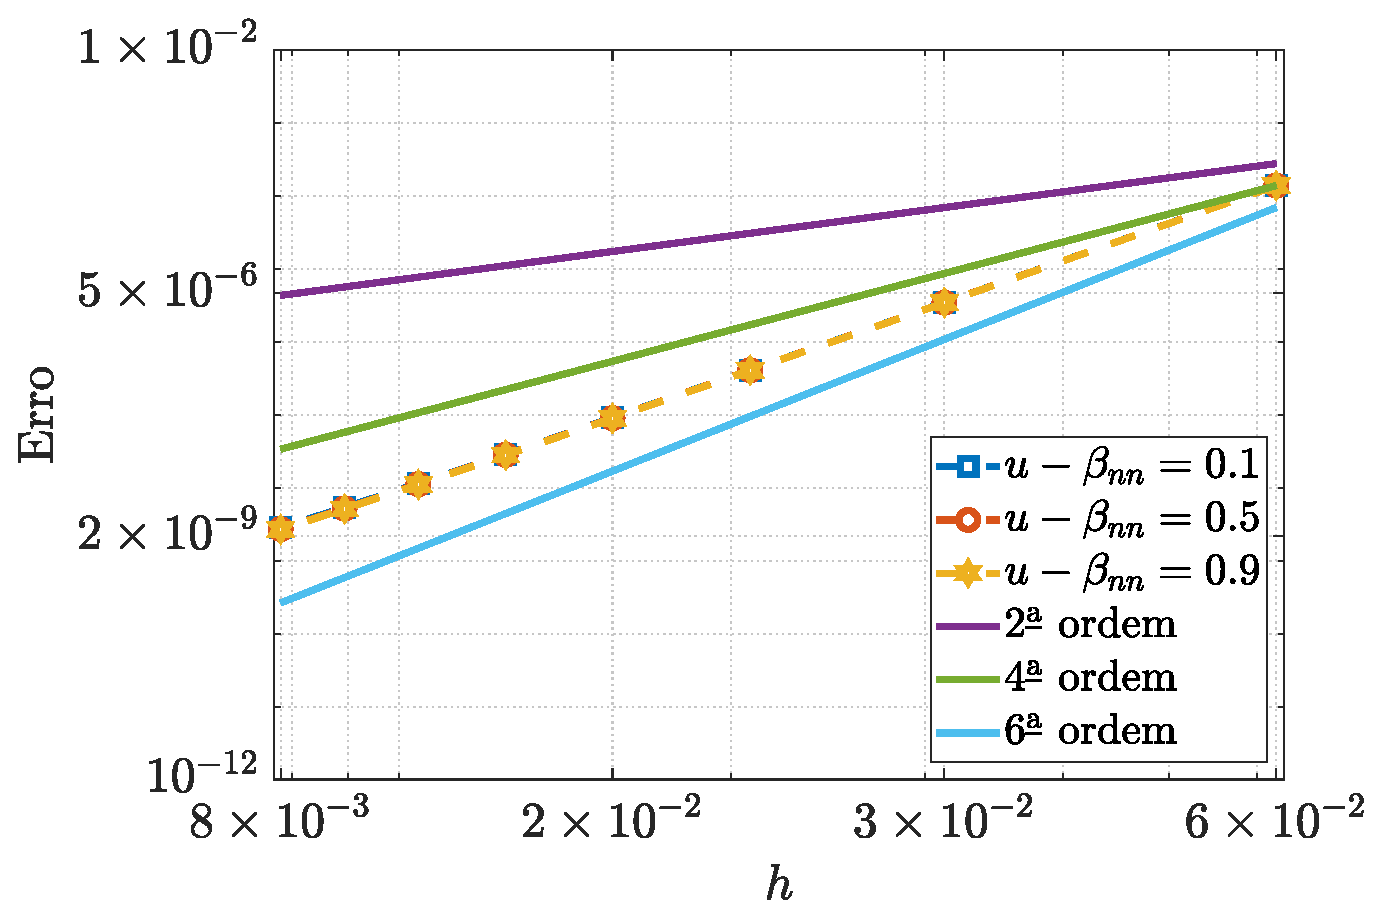
\includegraphics[width=\textwidth]{figures/Case12/OldroydB/Errors/NormErr_2nd_Re_100_Wi_1_epsilon_0_xi_0_alphaG_0_Dt_1e-06_at_0.05_tipsim_1_MMS_12_U.eps}
            \caption{$||U - \overline{u}||_{2}$}
            \label{error_u_2nd_Case1_oldorydb}
        \end{subfigure}
        \vspace{0.2cm}
        \qquad
        \begin{subfigure}[b]{.47\textwidth}
            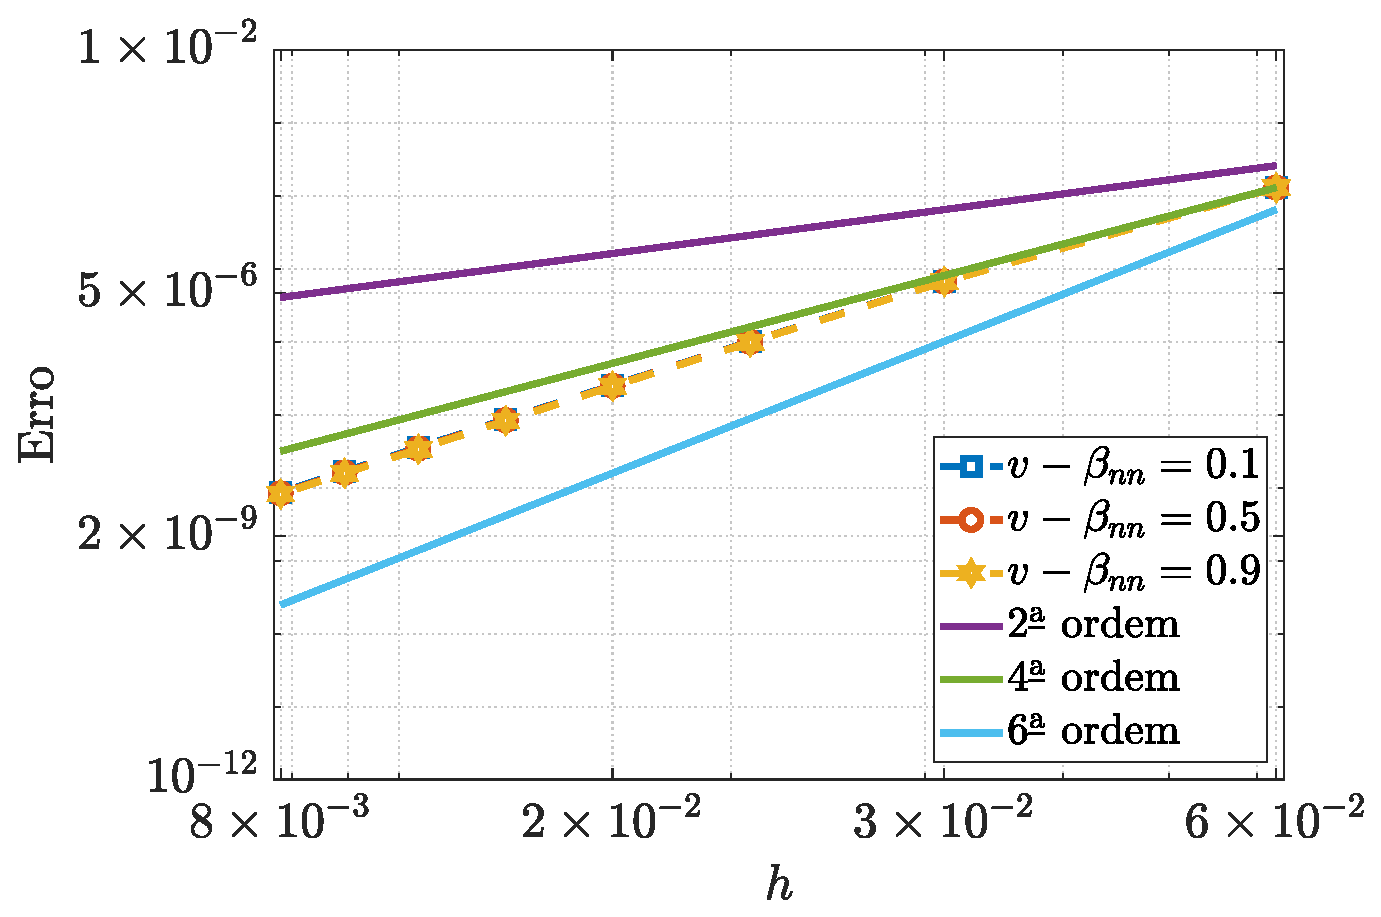
\includegraphics[width=\textwidth]{figures/Case12/OldroydB/Errors/NormErr_2nd_Re_100_Wi_1_epsilon_0_xi_0_alphaG_0_Dt_1e-06_at_0.05_tipsim_1_MMS_12_V.eps}
            \caption{$||V - \widetilde{v}||_{2}$}
            \label{error_v_2nd_Case1_oldorydb}
        \end{subfigure}
        \qquad
        \begin{subfigure}[b]{.47\textwidth}
            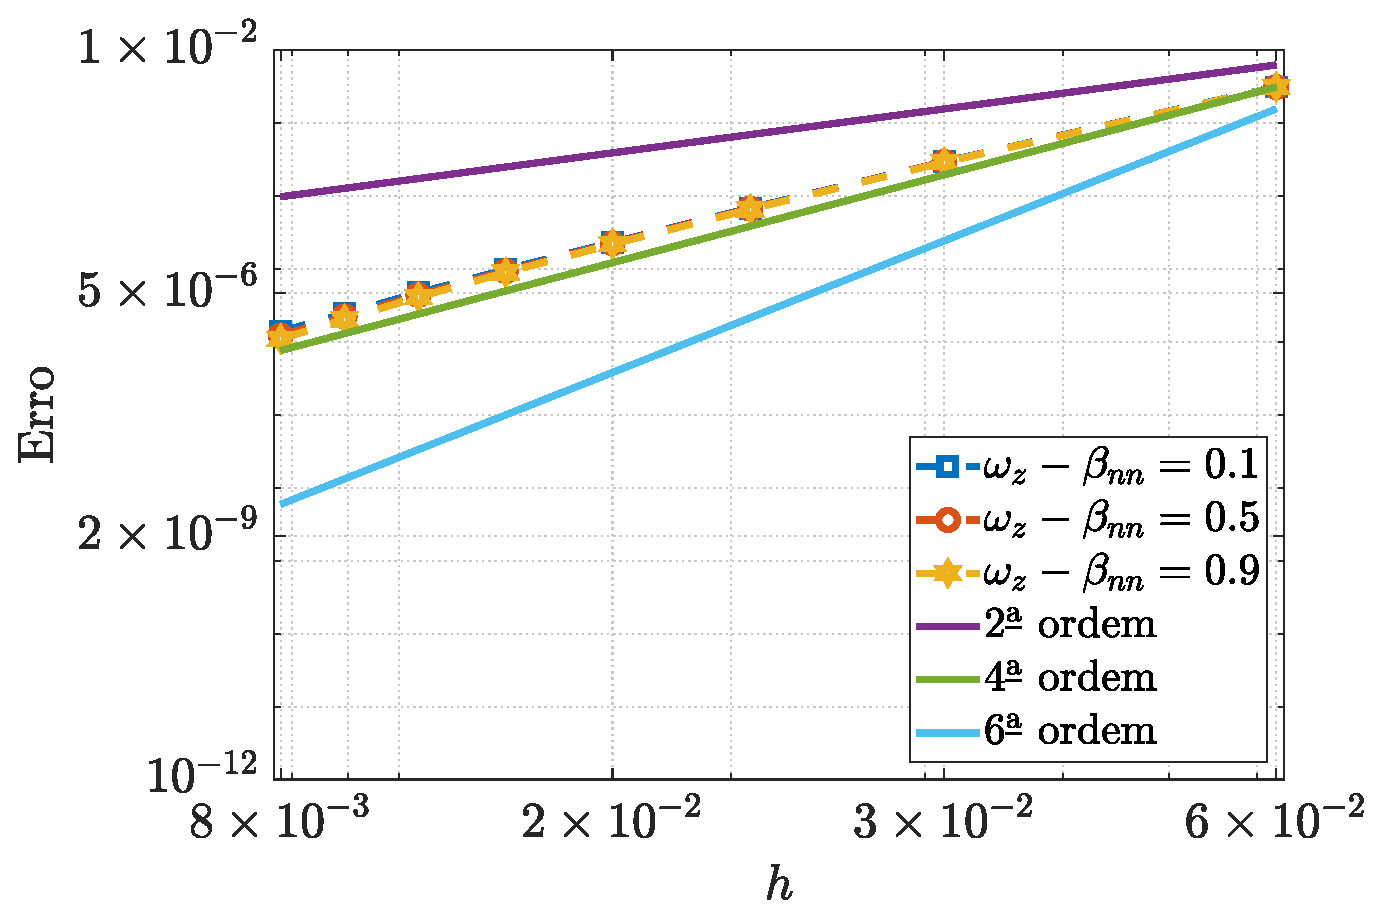
\includegraphics[width=\textwidth]{figures/Case12/OldroydB/Errors/NormErr_2nd_Re_100_Wi_1_epsilon_0_xi_0_alphaG_0_Dt_1e-06_at_0.05_tipsim_1_MMS_12_Wz.eps}
            \caption{$||\Omega_{z} - \widetilde{\omega_{z}}||_{2}$}
            \label{error_wz_2nd_Case1_oldorydb}
        \end{subfigure}
        \vspace{0.02cm}
        \qquad
        \begin{subfigure}[b]{.47\textwidth}
            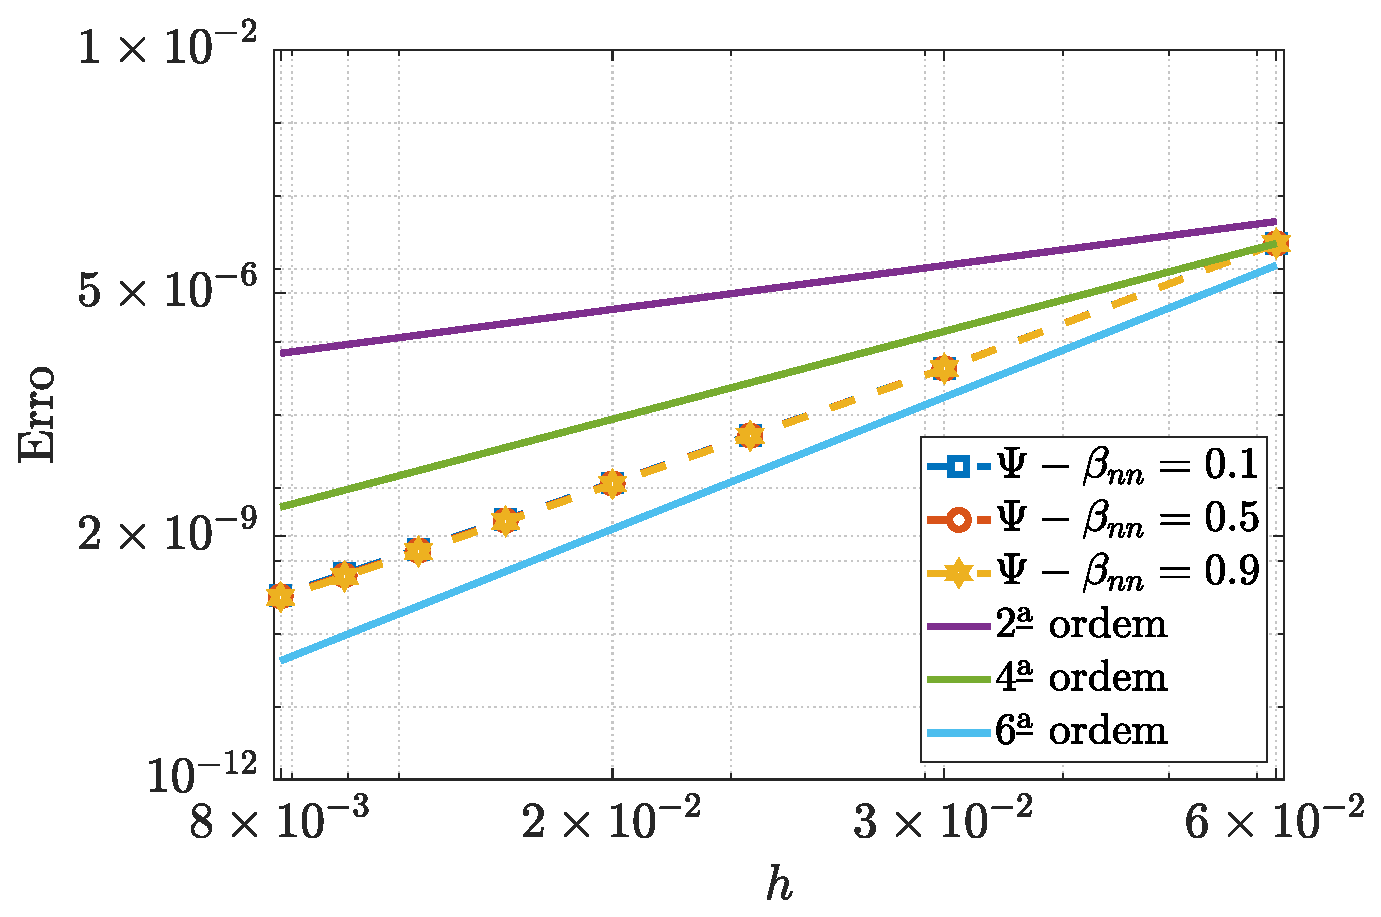
\includegraphics[width=\textwidth]{figures/Case12/OldroydB/Errors/NormErr_2nd_Re_100_Wi_1_epsilon_0_xi_0_alphaG_0_Dt_1e-06_at_0.05_tipsim_1_MMS_12_Psi.eps}
            \caption{$||\Psi - \widetilde{\Psi}||_{2}$}
            \label{error_psi_2nd_Case1_oldorydb}
        \end{subfigure}
        \fdadospesquisa
\end{figure}

\begin{figure}[H]
    \centering
    \caption{Erro para as componentes dos tensores de tensões, utilizando os parâmetros $Re=100$ e $Wi=1$, para o escoamento de fluido viscoelástico com o modelo Oldroyd-B}
    \label{OBerror2}
    \begin{subfigure}[b]{.47\textwidth}
        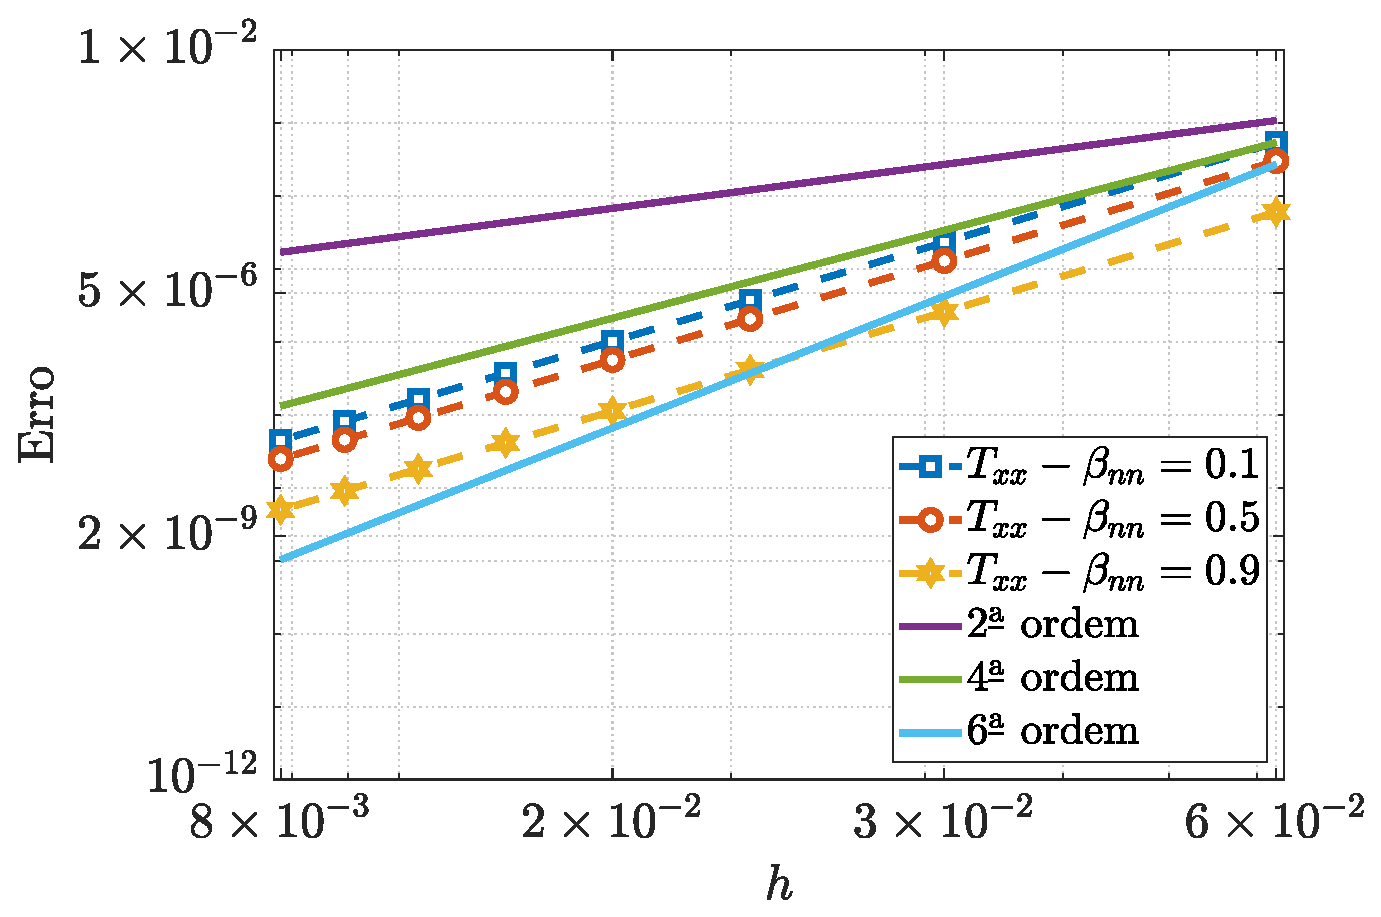
\includegraphics[width=\textwidth]{figures/Case12/OldroydB/Errors/NormErr_2nd_Re_100_Wi_1_epsilon_0_xi_0_alphaG_0_Dt_1e-06_at_0.05_tipsim_1_MMS_12_Txx.eps}
        \caption{$||T_{xx} - \overline{T}_{xx}||_{2}$}
        \label{error_txx_2nd_Case1_oldorydb}
    \end{subfigure}
    \vspace{0.2cm}
    \qquad
    \begin{subfigure}[b]{.47\textwidth}
        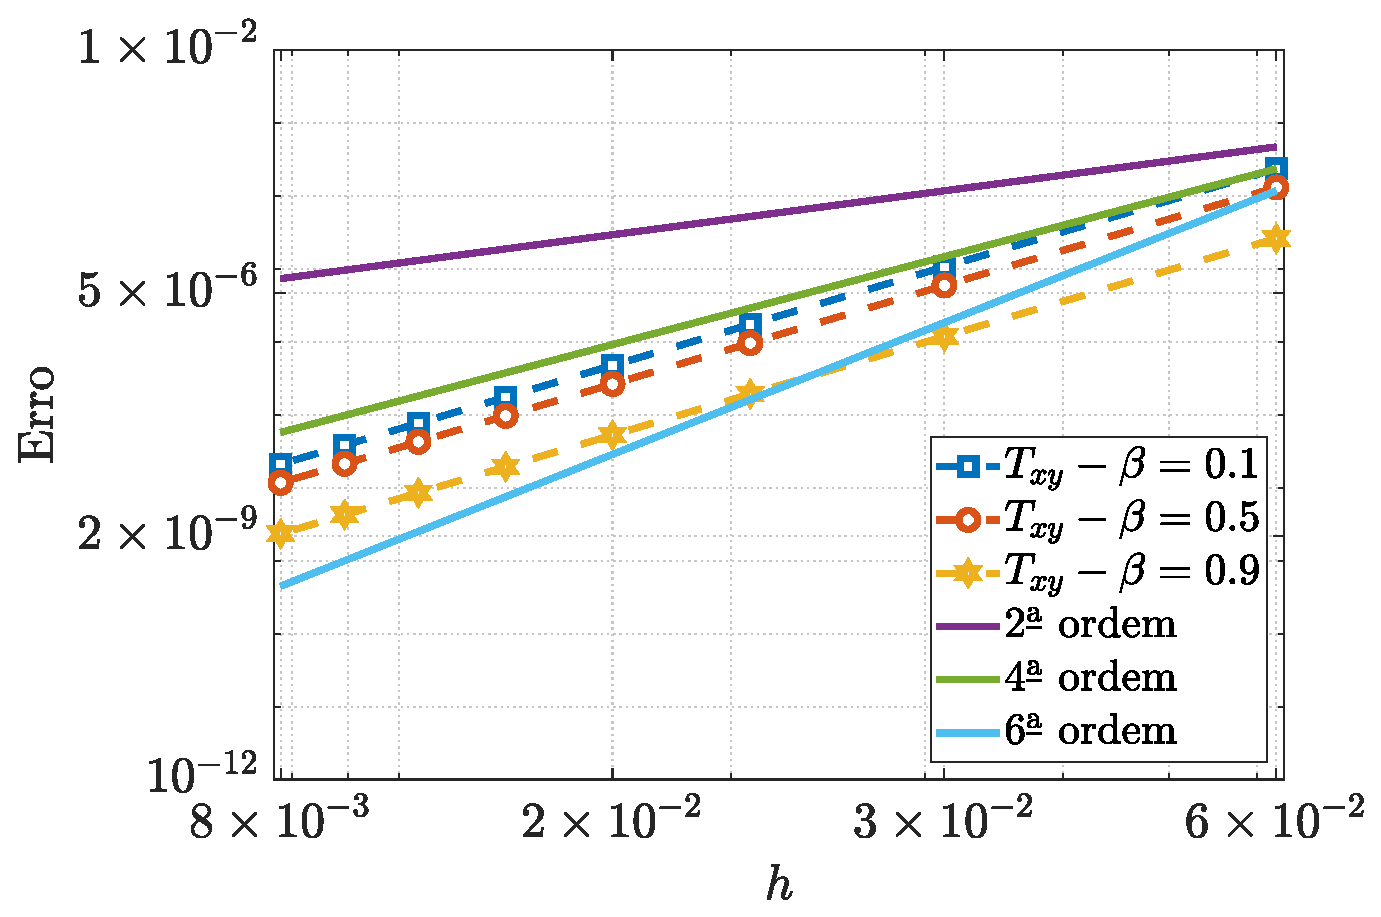
\includegraphics[width=\textwidth]{figures/Case12/OldroydB/Errors/NormErr_2nd_Re_100_Wi_1_epsilon_0_xi_0_alphaG_0_Dt_1e-06_at_0.05_tipsim_1_MMS_12_Txy.eps}
        \caption{$||T_{xy} - \overline{T}_{xy}||_{2}$}
        \label{error_txy_2nd_Case1_oldorydb}
    \end{subfigure}
    \qquad
    \begin{subfigure}[b]{.47\textwidth}
        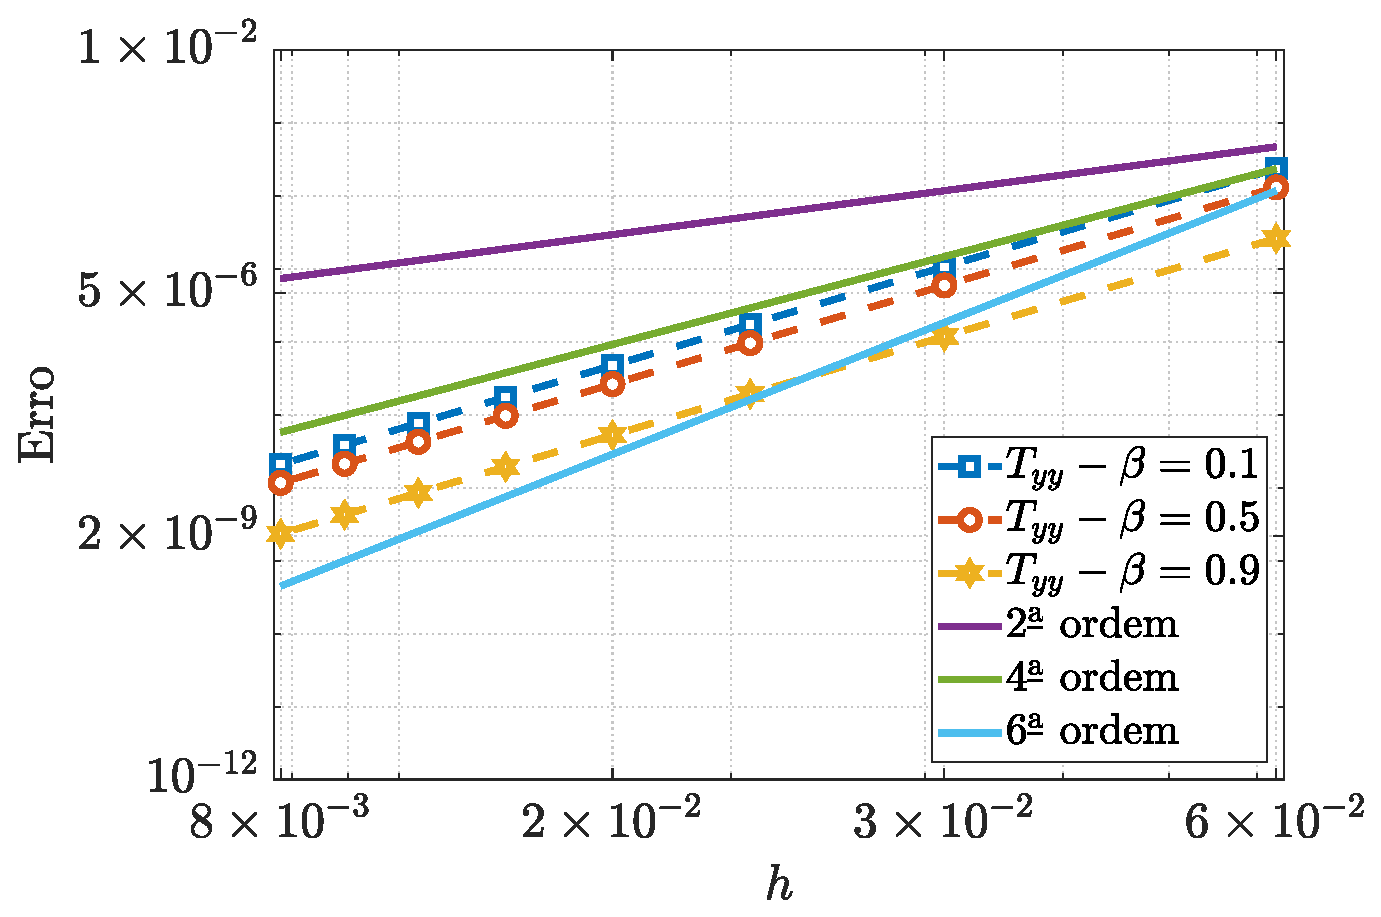
\includegraphics[width=\textwidth]{figures/Case12/OldroydB/Errors/NormErr_2nd_Re_100_Wi_1_epsilon_0_xi_0_alphaG_0_Dt_1e-06_at_0.05_tipsim_1_MMS_12_Tyy.eps}
        \caption{$||T_{yy} - \overline{T}_{yy}||_{2}$}
        \label{error_tyy_2nd_Case1_oldorydb}
    \end{subfigure}
    \fdadospesquisa
\end{figure}

As \autoref{OBerror1} e a \autoref{OBerror2} ilustram a ordem teórica de convergência obtida pelo código desenvolvido. Para proporcionar uma visão mais clara da convergência da vorticidade, a \autoref{tab_OldroydBWzResumida} apresenta os cálculos correspondentes para $Re = 1$, $100$, $400$, e $1000$, onde o comportamento discutido anteriormente pode ser claramente observado.
\begin{table}[H]
	\IBGEtab{
            \caption{Erros numéricos e cálculo da ordem de convergência para a vorticidade $(\omega_{z})$, utilizando o parâmetro $Wi=1$, para o escoamento de fluido viscoelástico Oldroyd-B}
            \label{tab_OldroydBWzResumida}
		}{
            \begin{tabular*}{\textwidth}{@{\extracolsep\fill}c|c|cc|cc|cc|cc@{}}
                \toprule
                 \multirow{2}{*}{$Re$} & \multirow{2}{*}{Malha} & \multicolumn{2}{c}{$\beta_{nn}=0.1$}  & \multicolumn{2}{c}{$\beta_{nn}=0.5$}  & \multicolumn{2}{c}{$\beta_{nn}=0.9$}  & \multicolumn{2}{c}{$\beta_{nn}=1.0$}\\ \cline{3-10}
                     & & Erro & p & Erro & p & Erro & p & Erro & p \\ \midrule
                    \multirow{7}{*}{1.00} & $17\times 17$ & 2.23e-03 & --- & 2.08e-03 & --- & 1.96e-03 & --- & 1.93e-03 & --- \\
                    & $33\times 33$ & 2.02e-04 & 3.47 & 1.51e-04 & 3.79 & 1.23e-04 & 4.00 & 1.18e-04 & 4.03 \\
                    & $49\times 49$ & 4.26e-05 & 3.84 & 2.50e-05 & 4.44 & 1.92e-05 & 4.57 & 1.84e-05 & 4.58 \\
                    & $65\times 65$ & 1.28e-05 & 4.17 & 6.43e-06 & 4.71 & 5.05e-06 & 4.65 & 4.85e-06 & 4.63 \\
                    & $81\times 81$ & 4.68e-06 & 4.52 & 2.23e-06 & 4.74 & 1.79e-06 & 4.63 & 1.73e-06 & 4.61 \\
                    & $97\times 97$ & 1.92e-06 & 4.90 & 9.34e-07 & 4.78 & 7.68e-07 & 4.65 & 7.45e-07 & 4.63 \\
                    & $113\times 113$ & 8.58e-07 & 5.21 & 4.47e-07 & 4.77 & 3.80e-07 & 4.57 & 3.71e-07 & 4.52 \\
                    & $129\times 129$ & 4.34e-07 & 5.10 & 2.59e-07 & 4.11 & 2.30e-07 & 3.76 & 2.26e-07 & 3.71 \\
                    \midrule
                    \multirow{7}{*}{100.00} & $17\times 17$ & 2.27e-03 & --- & 2.27e-03 & --- & 2.26e-03 & --- & 2.26e-03 & --- \\
                    & $33\times 33$ & 2.20e-04 & 3.37 & 2.19e-04 & 3.37 & 2.18e-04 & 3.37 & 2.18e-04 & 3.37 \\
                    & $49\times 49$ & 5.20e-05 & 3.56 & 5.15e-05 & 3.57 & 5.11e-05 & 3.58 & 5.10e-05 & 3.59 \\
                    & $65\times 65$ & 1.82e-05 & 3.66 & 1.79e-05 & 3.68 & 1.76e-05 & 3.70 & 1.75e-05 & 3.71 \\
                    & $81\times 81$ & 7.84e-06 & 3.76 & 7.65e-06 & 3.80 & 7.47e-06 & 3.84 & 7.43e-06 & 3.85 \\
                    & $97\times 97$ & 3.83e-06 & 3.93 & 3.70e-06 & 3.99 & 3.57e-06 & 4.05 & 3.54e-06 & 4.06 \\
                    & $113\times 113$ & 2.04e-06 & 4.10 & 1.94e-06 & 4.19 & 1.85e-06 & 4.27 & 1.83e-06 & 4.29 \\
                    & $129\times 129$ & 1.21e-06 & 3.89 & 1.13e-06 & 4.02 & 1.07e-06 & 4.13 & 1.05e-06 & 4.16 \\
                    \midrule
                    \multirow{7}{*}{400.00} & $17\times 17$ & 2.27e-03 & --- & 2.27e-03 & --- & 2.27e-03 & --- & 2.27e-03 & --- \\
                    & $33\times 33$ & 2.20e-04 & 3.37 & 2.20e-04 & 3.37 & 2.20e-04 & 3.37 & 2.20e-04 & 3.37 \\
                    & $49\times 49$ & 5.21e-05 & 3.56 & 5.19e-05 & 3.56 & 5.18e-05 & 3.56 & 5.18e-05 & 3.56 \\
                    & $65\times 65$ & 1.82e-05 & 3.65 & 1.81e-05 & 3.66 & 1.81e-05 & 3.66 & 1.81e-05 & 3.66 \\
                    & $81\times 81$ & 7.88e-06 & 3.75 & 7.83e-06 & 3.76 & 7.79e-06 & 3.77 & 7.78e-06 & 3.77 \\
                    & $97\times 97$ & 3.86e-06 & 3.92 & 3.83e-06 & 3.93 & 3.80e-06 & 3.94 & 3.79e-06 & 3.95 \\
                    & $113\times 113$ & 2.05e-06 & 4.09 & 2.03e-06 & 4.11 & 2.01e-06 & 4.12 & 2.01e-06 & 4.13 \\
                    & $129\times 129$ & 1.23e-06 & 3.86 & 1.21e-06 & 3.89 & 1.19e-06 & 3.92 & 1.19e-06 & 3.93 \\
                    \midrule
                    \multirow{7}{*}{1000.00} & $17\times 17$ & 2.27e-03 & --- & 2.27e-03 & --- & 2.27e-03 & --- & 2.27e-03 & --- \\
                    & $33\times 33$ & 2.20e-04 & 3.37 & 2.20e-04 & 3.37 & 2.20e-04 & 3.37 & 2.20e-04 & 3.37 \\
                    & $49\times 49$ & 5.21e-05 & 3.56 & 5.20e-05 & 3.56 & 5.20e-05 & 3.56 & 5.20e-05 & 3.56 \\
                    & $65\times 65$ & 1.82e-05 & 3.65 & 1.82e-05 & 3.65 & 1.82e-05 & 3.65 & 1.82e-05 & 3.65 \\
                    & $81\times 81$ & 7.89e-06 & 3.75 & 7.87e-06 & 3.76 & 7.86e-06 & 3.76 & 7.85e-06 & 3.76 \\
                    & $97\times 97$ & 3.86e-06 & 3.92 & 3.85e-06 & 3.92 & 3.84e-06 & 3.92 & 3.84e-06 & 3.92 \\
                    & $113\times 113$ & 2.06e-06 & 4.08 & 2.05e-06 & 4.09 & 2.04e-06 & 4.09 & 2.04e-06 & 4.09 \\
                    & $129\times 129$ & 1.23e-06 & 3.86 & 1.22e-06 & 3.87 & 1.22e-06 & 3.87 & 1.22e-06 & 3.88 \\
                    \bottomrule
                \end{tabular*}
		}{
		\fdadospesquisa
	}
\end{table}

Na \autoref{tab_OldroydBWzResumida}, os erros de vorticidade são apresentados para números de Reynolds ($Re$) iguais a 1, 100, 400 e 1000, considerando diferentes razões de viscosidade do solvente ($\beta_{nn} = 0.1,\ 0.5,\ 0.9$ e $1$). À medida que a malha é refinada, os erros diminuem consistentemente, com a ordem de convergência $p$ aproximando-se de 4.5, como esperado para métodos numéricos de alta ordem. A consistência na taxa de convergência para todos os números de Reynolds e razões de viscosidade reforça a precisão e a robustez do modelo.
\begin{table}[H]
	\IBGEtab{
            \caption{Erros numéricos e cálculo da ordem de convergência para a componente do tensor de tensões $T_{xx}$, utilizando o parâmetro $Wi=1$, para o escoamento de fluido viscoelástico Oldroyd-B}
            \label{tab_OldroydBTxxResumida}
		}{
		\begin{tabular*}{\textwidth}{@{\extracolsep\fill}c|c|cc|cc|cc|cc@{}}
                \toprule
                \multirow{2}{*}{$Re$} & \multirow{2}{*}{Malha} & \multicolumn{2}{c}{$\beta_{nn}=0.1$}  & \multicolumn{2}{c}{$\beta_{nn}=0.5$}  & \multicolumn{2}{c}{$\beta_{nn}=0.9$}  & \multicolumn{2}{c}{$\beta_{nn}=1.0$}  \\
                \cline{3-10}
                 & & Erro & p & Erro & p & Erro & p & Erro & p \\ \midrule
                \multirow{10}{*}{1.00} & 17$\times$17 & 5.38e-04 & --- & 2.99e-04 & --- & 5.97e-05 & --- & 5.97e-18 & --- \\
                & 33$\times$33 & 2.30e-05 & 4.54 & 1.28e-05 & 4.54 & 2.56e-06 & 4.54 & 2.56e-19 & 4.54 \\
                & 49$\times$49 & 3.69e-06 & 4.52 & 2.05e-06 & 4.52 & 4.10e-07 & 4.52 & 4.10e-20 & 4.52 \\
                & 65$\times$65 & 1.01e-06 & 4.51 & 5.61e-07 & 4.51 & 1.12e-07 & 4.51 & 1.12e-20 & 4.51 \\
                & 81$\times$81 & 3.69e-07 & 4.50 & 2.05e-07 & 4.50 & 4.10e-08 & 4.50 & 4.10e-21 & 4.50 \\
                & 97$\times$97 & 1.62e-07 & 4.50 & 9.03e-08 & 4.50 & 1.80e-08 & 4.50 & 1.80e-21 & 4.50 \\
                & 113$\times$113 & 8.12e-08 & 4.50 & 4.51e-08 & 4.50 & 9.02e-09 & 4.50 & 9.01e-22 & 4.50 \\
                & 129$\times$129 & 4.45e-08 & 4.50 & 2.47e-08 & 4.50 & 4.94e-09 & 4.50 & 4.94e-22 & 4.50 \\
                \midrule
                \multirow{10}{*}{100.00} & 17$\times$17 & 5.38e-04 & --- & 2.99e-04 & --- & 5.97e-05 & --- & 5.97e-18 & --- \\
                & 33$\times$33 & 2.30e-05 & 4.54 & 1.28e-05 & 4.54 & 2.56e-06 & 4.54 & 2.56e-19 & 4.54 \\
                & 49$\times$49 & 3.69e-06 & 4.52 & 2.05e-06 & 4.52 & 4.10e-07 & 4.52 & 4.10e-20 & 4.52 \\
                & 65$\times$65 & 1.01e-06 & 4.51 & 5.61e-07 & 4.51 & 1.12e-07 & 4.51 & 1.12e-20 & 4.51 \\
                & 81$\times$81 & 3.69e-07 & 4.50 & 2.05e-07 & 4.50 & 4.10e-08 & 4.50 & 4.10e-21 & 4.50 \\
                & 97$\times$97 & 1.62e-07 & 4.50 & 9.03e-08 & 4.50 & 1.81e-08 & 4.50 & 1.80e-21 & 4.50 \\
                & 113$\times$113 & 8.12e-08 & 4.50 & 4.51e-08 & 4.50 & 9.02e-09 & 4.50 & 9.01e-22 & 4.50 \\
                & 129$\times$129 & 4.45e-08 & 4.50 & 2.47e-08 & 4.50 & 4.94e-09 & 4.50 & 4.94e-22 & 4.50 \\
                \midrule
                \multirow{10}{*}{400.00} & 17$\times$17 & 5.38e-04 & --- & 2.99e-04 & --- & 5.97e-05 & --- & 5.97e-18 & --- \\
                & 33$\times$33 & 2.30e-05 & 4.54 & 1.28e-05 & 4.54 & 2.56e-06 & 4.54 & 2.56e-19 & 4.54 \\
                & 49$\times$49 & 3.69e-06 & 4.52 & 2.05e-06 & 4.52 & 4.10e-07 & 4.52 & 4.10e-20 & 4.52 \\
                & 65$\times$65 & 1.01e-06 & 4.51 & 5.61e-07 & 4.51 & 1.12e-07 & 4.51 & 1.12e-20 & 4.51 \\
                & 81$\times$81 & 3.69e-07 & 4.50 & 2.05e-07 & 4.50 & 4.10e-08 & 4.50 & 4.10e-21 & 4.50 \\
                & 97$\times$97 & 1.62e-07 & 4.50 & 9.03e-08 & 4.50 & 1.81e-08 & 4.50 & 1.80e-21 & 4.50 \\
                & 113$\times$113 & 8.11e-08 & 4.50 & 4.51e-08 & 4.50 & 9.02e-09 & 4.50 & 9.01e-22 & 4.50 \\
                & 129$\times$129 & 4.45e-08 & 4.50 & 2.47e-08 & 4.50 & 4.94e-09 & 4.50 & 4.94e-22 & 4.50 \\
                \midrule
                \multirow{10}{*}{1000.00} & 17$\times$17 & 5.38e-04 & --- & 2.99e-04 & --- & 5.97e-05 & --- & 5.97e-18 & --- \\
                & 33$\times$33 & 2.30e-05 & 4.54 & 1.28e-05 & 4.54 & 2.56e-06 & 4.54 & 2.56e-19 & 4.54 \\
                & 49$\times$49 & 3.69e-06 & 4.52 & 2.05e-06 & 4.52 & 4.10e-07 & 4.52 & 4.10e-20 & 4.52 \\
                & 65$\times$65 & 1.01e-06 & 4.51 & 5.61e-07 & 4.51 & 1.12e-07 & 4.51 & 1.12e-20 & 4.51 \\
                & 81$\times$81 & 3.69e-07 & 4.50 & 2.05e-07 & 4.50 & 4.10e-08 & 4.50 & 4.10e-21 & 4.50 \\
                & 97$\times$97 & 1.62e-07 & 4.50 & 9.03e-08 & 4.50 & 1.81e-08 & 4.50 & 1.80e-21 & 4.50 \\
                & 113$\times$113 & 8.11e-08 & 4.50 & 4.51e-08 & 4.50 & 9.02e-09 & 4.50 & 9.01e-22 & 4.50 \\
                & 129$\times$129 & 4.45e-08 & 4.50 & 2.47e-08 & 4.50 & 4.94e-09 & 4.50 & 4.94e-22 & 4.50 \\
                \bottomrule
            \end{tabular*}
		}{
		\fdadospesquisa
	}
\end{table}

A \autoref{tab_OldroydBTxxResumida} apresenta os erros e as ordens de convergência para o componente $T_{xx}$ do tensor de tensões extra. Similarmente aos resultados da vorticidade, observa-se uma redução clara nos erros à medida que a malha é refinada, com a ordem de convergência permanecendo próxima de 4.5 em todas as condições avaliadas. Esses resultados indicam a estabilidade e robustez do método numérico, tanto na simulação da vorticidade quanto nas tensões extras. Ao examinar a tabela, para $\beta_{nn} = 1$, fica evidente que os erros numéricos são extremamente pequenos, aproximando-se dos níveis de precisão de máquina (por exemplo, $5.97e-18$ ou $4.94e-22$). Esse comportamento é esperado, visto que $\beta_{nn} = 1$ corresponde ao caso de um fluido Newtoniano, onde os tensores de tensões extras como $T_{xx}$ se tornam aproximadamente nulos. Como resultado, os erros são mínimos e a ordem de convergência permanece consistentemente em torno de 4.5, alinhando-se com o desempenho esperado para métodos numéricos de alta ordem. Os erros quase nulos para $\beta_{nn} = 1$ demonstram que o esquema numérico captura com precisão o caso limite de um fluido Newtoniano.

\subsection{Caso de verificação usando o modelo Giesekus}

Nas simulações realizadas com o modelo de Giesekus, foram utilizados números de Reynolds variando de $Re = 1,\ 10,\ 100,\ 400$ e $1000$, com o número de Weissenberg mantido fixo em $Wi = 1$, e diferentes razões de viscosidade do solvente $\beta_{nn} = 0.1,\ 0.5,\ 0.9$ e $1$. Além disso, o parâmetro $\alpha_G$ foi ajustado para valores de $0.1$, $0.5$ e $0.85$, visando analisar o comportamento do modelo sob diferentes regimes de escoamento. A análise de erro foi conduzida para avaliar o desempenho do método em relação ao campo de velocidade, vorticidade, função de corrente e tensores de tensões extras.

Na \autoref{GEerror011}, são apresentados os gráficos de erro para os componentes do campo de velocidade, vorticidade e função de corrente, considerando o modelo de Giesekus com $Re = 100$, $Wi = 1$ e $\alpha_G = 0.1$. Como demonstrado, os erros diminuem consistentemente à medida que a malha é refinada. A ordem de convergência $p$ aproxima-se de 4.5, conforme esperado para métodos numéricos de alta ordem. Esse comportamento consistente reforça a robustez e a precisão do esquema numérico, demonstrando sua eficácia na captura das dinâmicas de fluidos viscoelásticos sob diferentes razões de viscosidade do solvente. Essa análise é fundamental para validar a capacidade do modelo em simular corretamente diferentes propriedades do escoamento.
\begin{figure}[H] 
    \centering
    \caption{Erro para o campo de velocidade $(\overline{u},\tilde{v})$, vorticidade $(\tilde{\omega_{z}})$ e função de corrente $(\tilde{\psi})$, considerando $Re=100$, $Wi=1$ e $\alpha_G=0.1$, para o escoamento de fluido viscoelástico com o modelo Giesekus}\label{GEerror011}
    \begin{subfigure}[b]{.47\textwidth}
        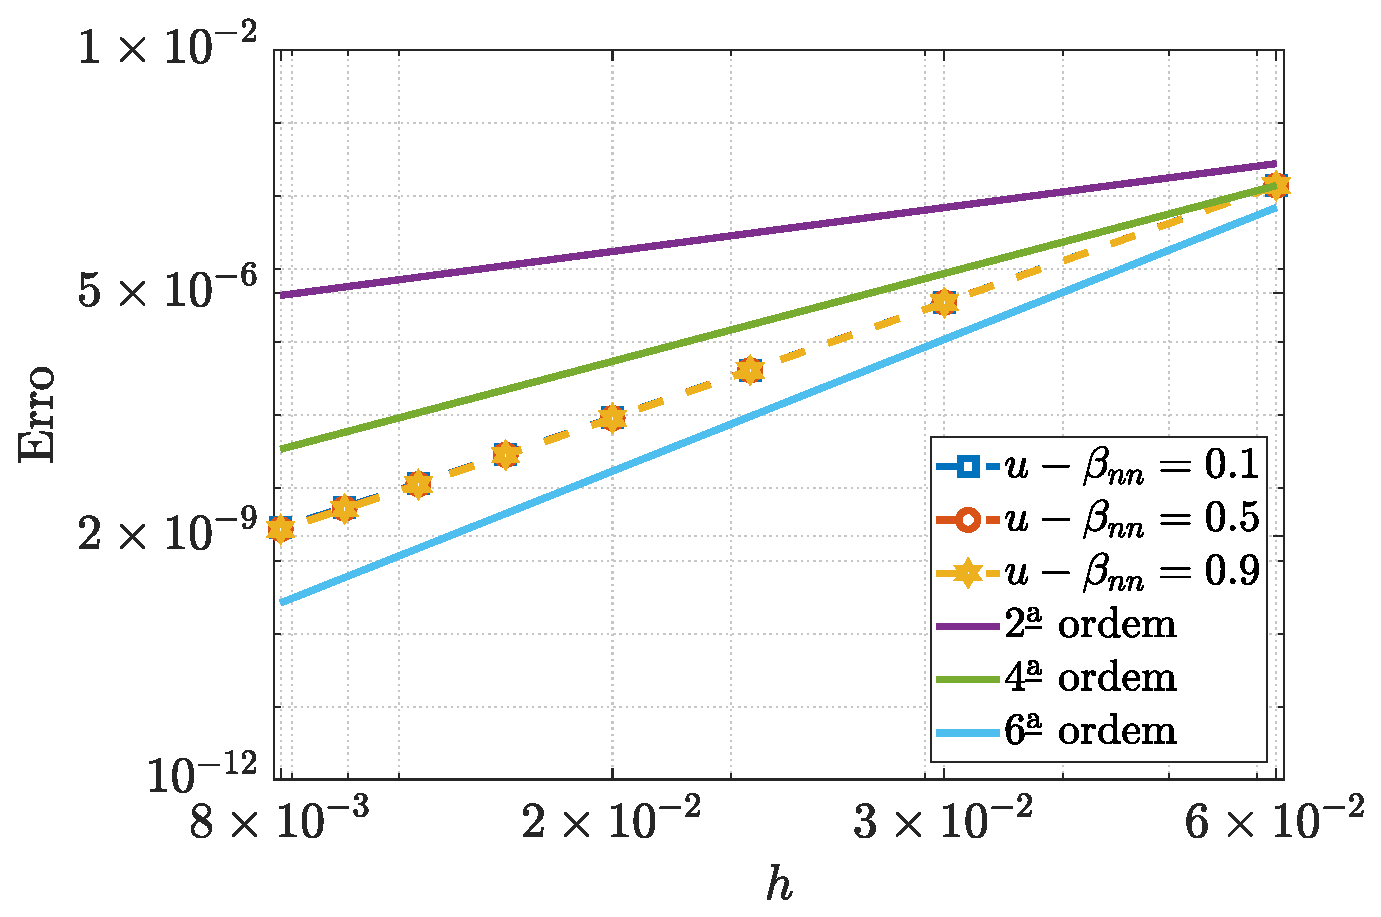
\includegraphics[width=\textwidth]{figures/Case12/Giesekus/Errors/NormErr_2nd_Re_100_Wi_1_epsilon_0_xi_0_alphaG_0.1_Dt_1e-06_at_0.05_tipsim_1_MMS_12_U.eps}
        \caption{$||U - \overline{u}||_{2}$}
        \label{error_u_2nd_Case1_giesekus_alphaG_0.1}
    \end{subfigure}
    \vspace{0.2cm}
    \qquad
    \begin{subfigure}[b]{.47\textwidth}
        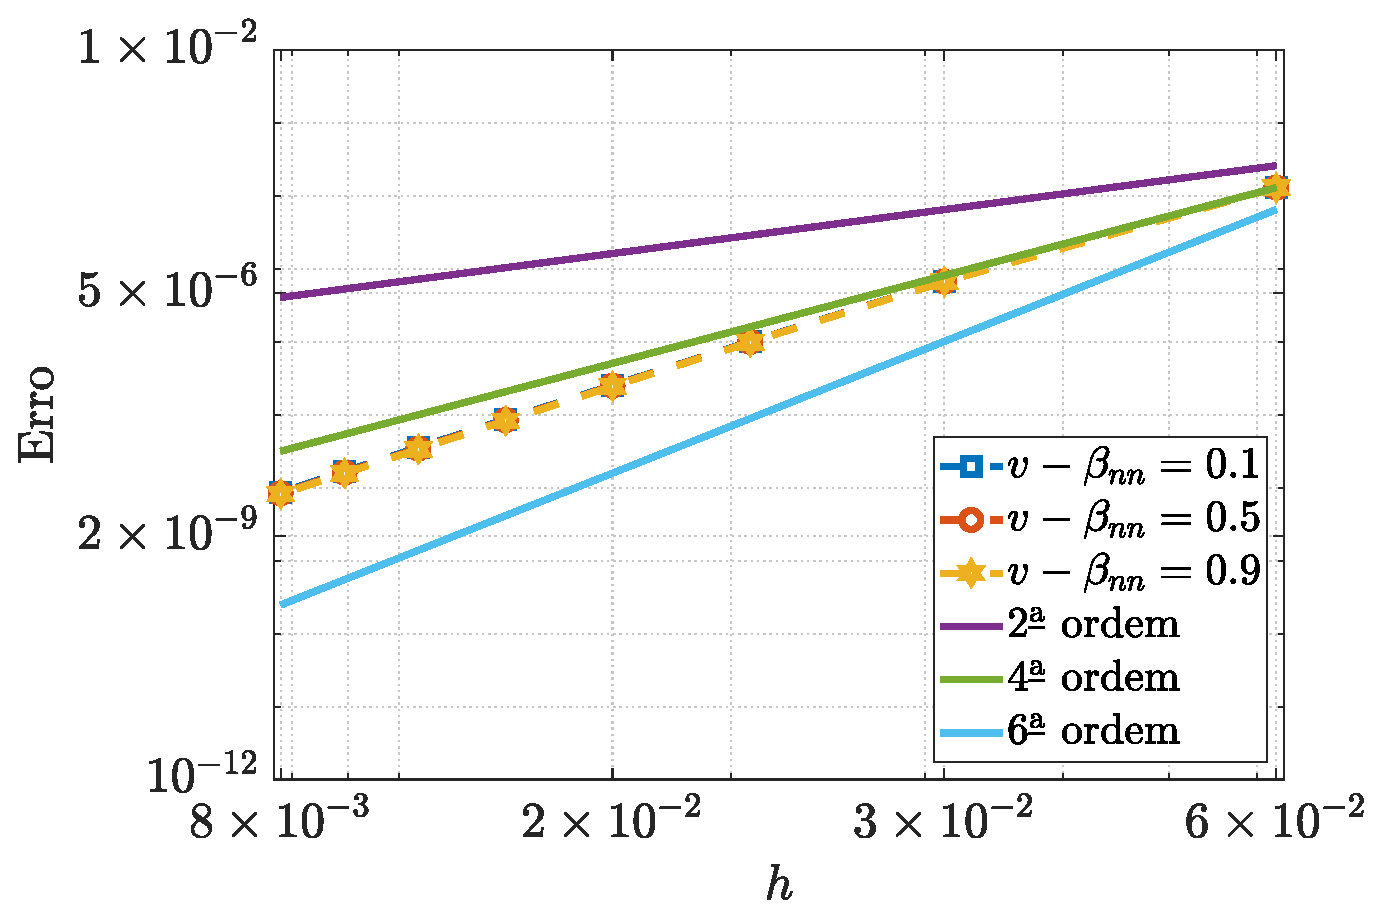
\includegraphics[width=\textwidth]{figures/Case12/Giesekus/Errors/NormErr_2nd_Re_100_Wi_1_epsilon_0_xi_0_alphaG_0.1_Dt_1e-06_at_0.05_tipsim_1_MMS_12_V.eps}
        \caption{$||V - \widetilde{v}||_{2}$}
        \label{error_v_2nd_Case1_giesekus_alphaG_0.1}
    \end{subfigure}
    \qquad
    \begin{subfigure}[b]{.47\textwidth}
        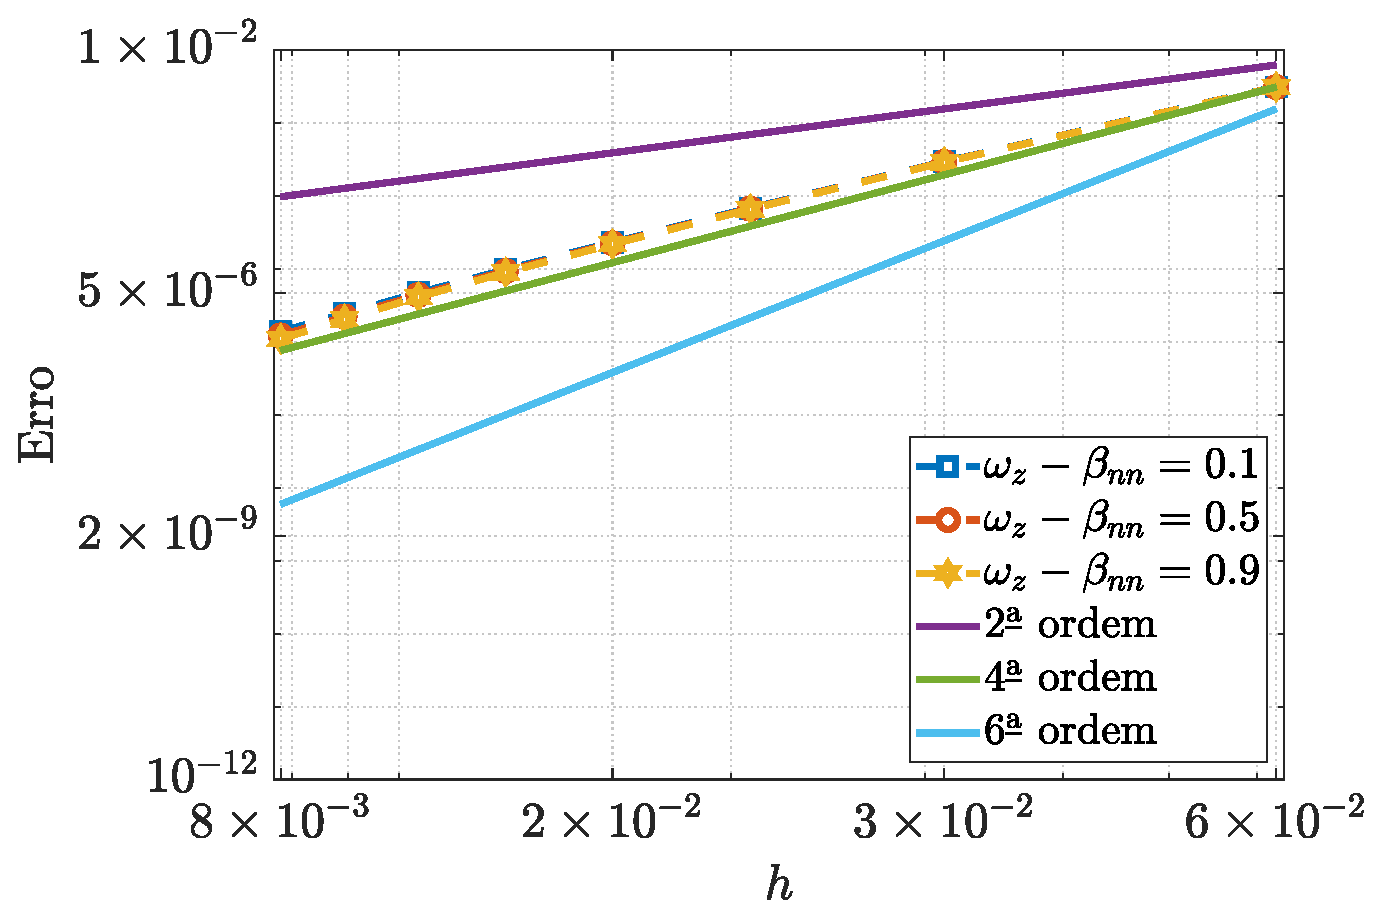
\includegraphics[width=\textwidth]{figures/Case12/Giesekus/Errors/NormErr_2nd_Re_100_Wi_1_epsilon_0_xi_0_alphaG_0.1_Dt_1e-06_at_0.05_tipsim_1_MMS_12_Wz.eps}
        \caption{$||\Omega_{z} - \widetilde{\omega_{z}}||_{2}$}
        \label{error_wz_2nd_Case1_giesekus_alphaG_0.1}
    \end{subfigure}
    \qquad
    \begin{subfigure}[b]{.47\textwidth}
        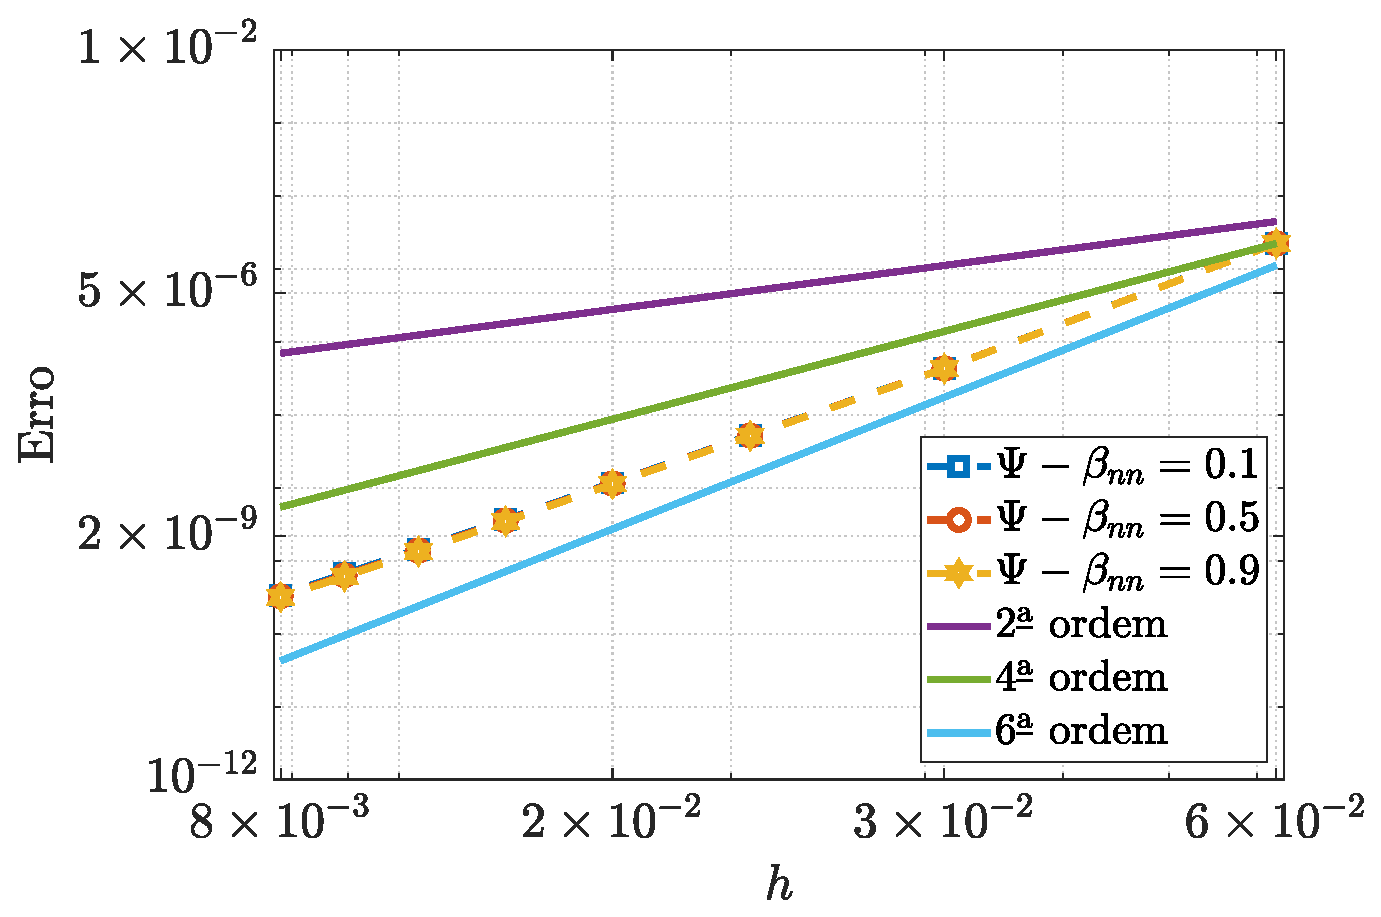
\includegraphics[width=\textwidth]{figures/Case12/Giesekus/Errors/NormErr_2nd_Re_100_Wi_1_epsilon_0_xi_0_alphaG_0.1_Dt_1e-06_at_0.05_tipsim_1_MMS_12_Psi.eps}
        \caption{$||\Psi - \widetilde{\Psi}||_{2}$}
        \label{error_psi_2nd_Case1_oldorydbgiesekus_alphaG_0.1}
    \end{subfigure}
    \fautor
\end{figure}

A \autoref{GEerror012} amplia a análise ao apresentar os erros relacionados à conformidade dos tensores extra-tensões $T_{xx}$, $T_{xy}$ e $T_{yy}$, para o mesmo conjunto de parâmetros $Re = 100$, $Wi = 1$ e $\alpha_G = 0.1$. Os resultados indicam uma redução significativa nos erros à medida que a malha é refinada, mantendo uma alta ordem de convergência, geralmente próxima de 4,5. Isso sugere que o método numérico é robusto na captura da complexidade das tensões extras em fluidos viscoelásticos, minimizando as discrepâncias para diferentes valores de $\beta_{nn}$.
\begin{figure}[H]
    \centering
    \caption{Erro para os componentes tensores extra-tensão, usando os parâmetros $Re=100,$ $Wi=1$ e $\alpha_{G} = 0.1$, para o fluxo de fluido viscoelástico com o modelo Giesekus}\label{GEerror012}
    \begin{subfigure}[b]{.47\textwidth}
        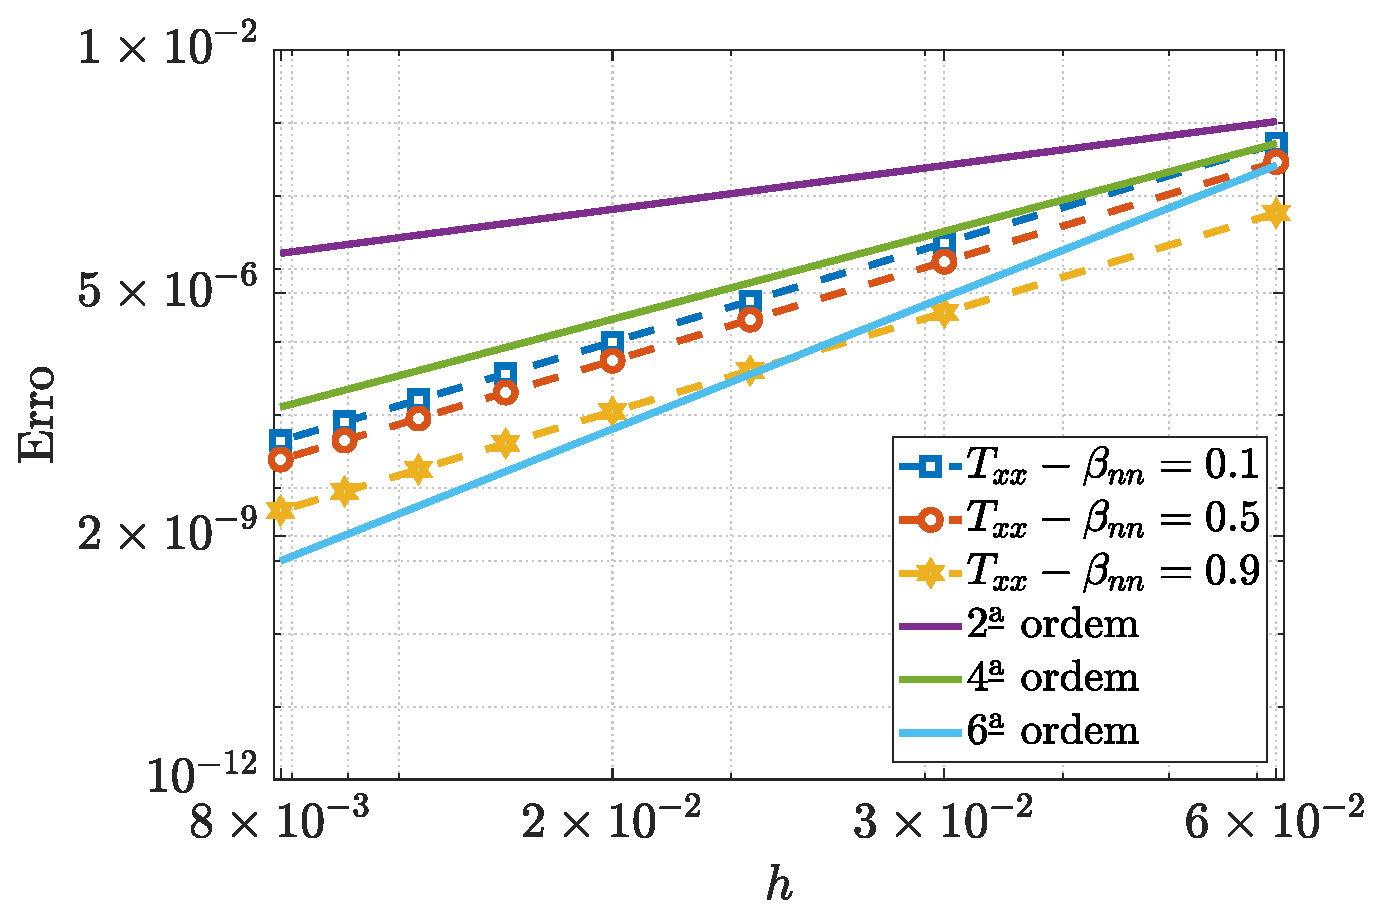
\includegraphics[width=\textwidth]{figures/Case12/Giesekus/Errors/NormErr_2nd_Re_100_Wi_1_epsilon_0_xi_0_alphaG_0.1_Dt_1e-06_at_0.05_tipsim_1_MMS_12_Txx.eps}
        \caption{$||T_{xx} - \overline{T}_{xx}||_{2}$}
        \label{error_txx_2nd_Case1_giesekus_alphaG_0.1}
    \end{subfigure}
    \vspace{0.2cm}
    \qquad
    \begin{subfigure}[b]{.47\textwidth}
        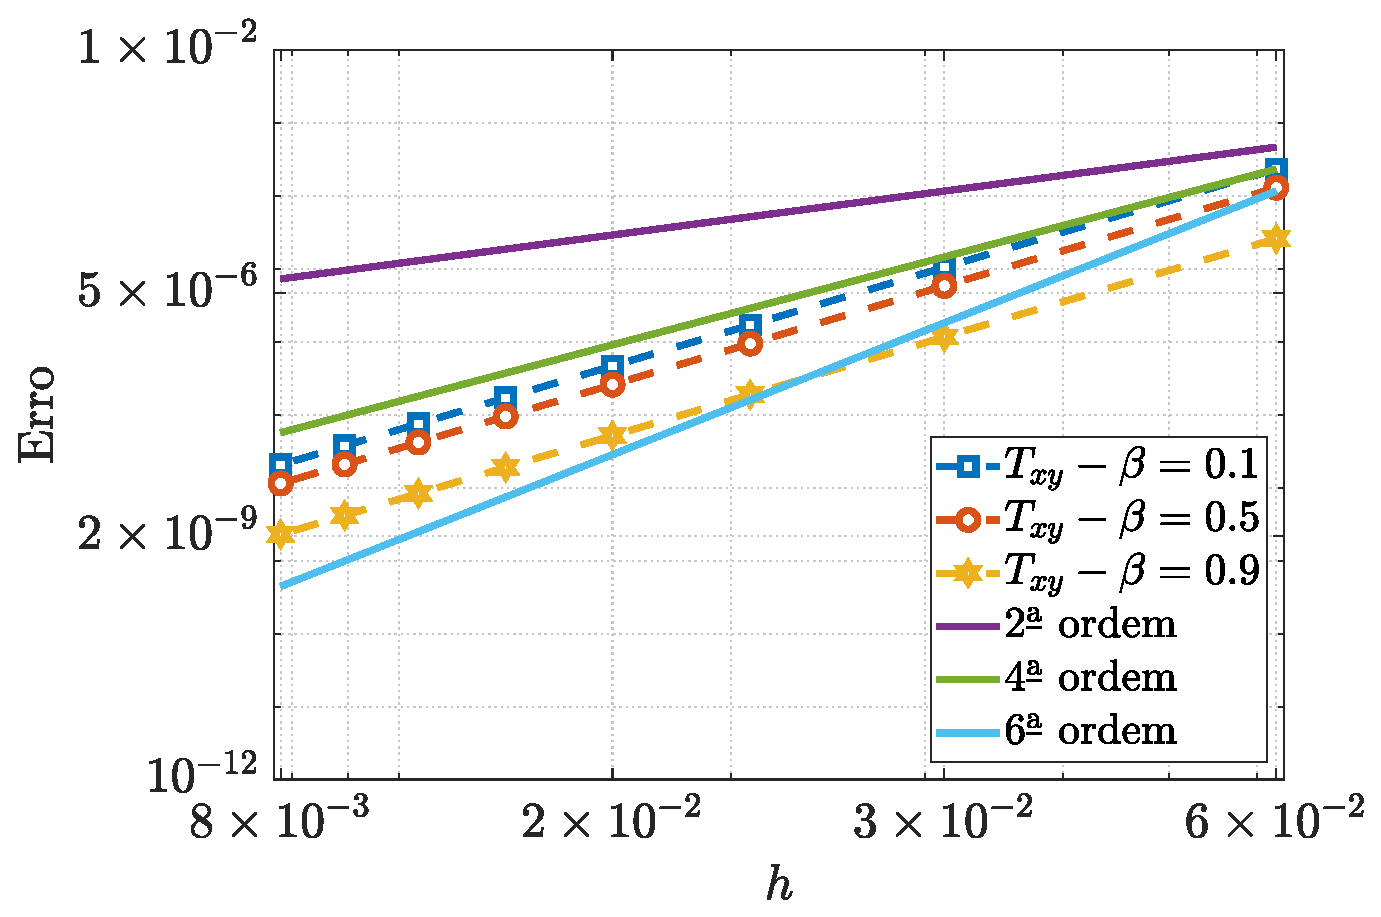
\includegraphics[width=\textwidth]{figures/Case12/Giesekus/Errors/NormErr_2nd_Re_100_Wi_1_epsilon_0_xi_0_alphaG_0.1_Dt_1e-06_at_0.05_tipsim_1_MMS_12_Txy.eps}
        \caption{$||T_{xy} - \overline{T}_{xy}||_{2}$}
        \label{error_txy_2nd_Case1_giesekus_alphaG_0.1}
    \end{subfigure}
    \qquad
    \begin{subfigure}[b]{.47\textwidth}
        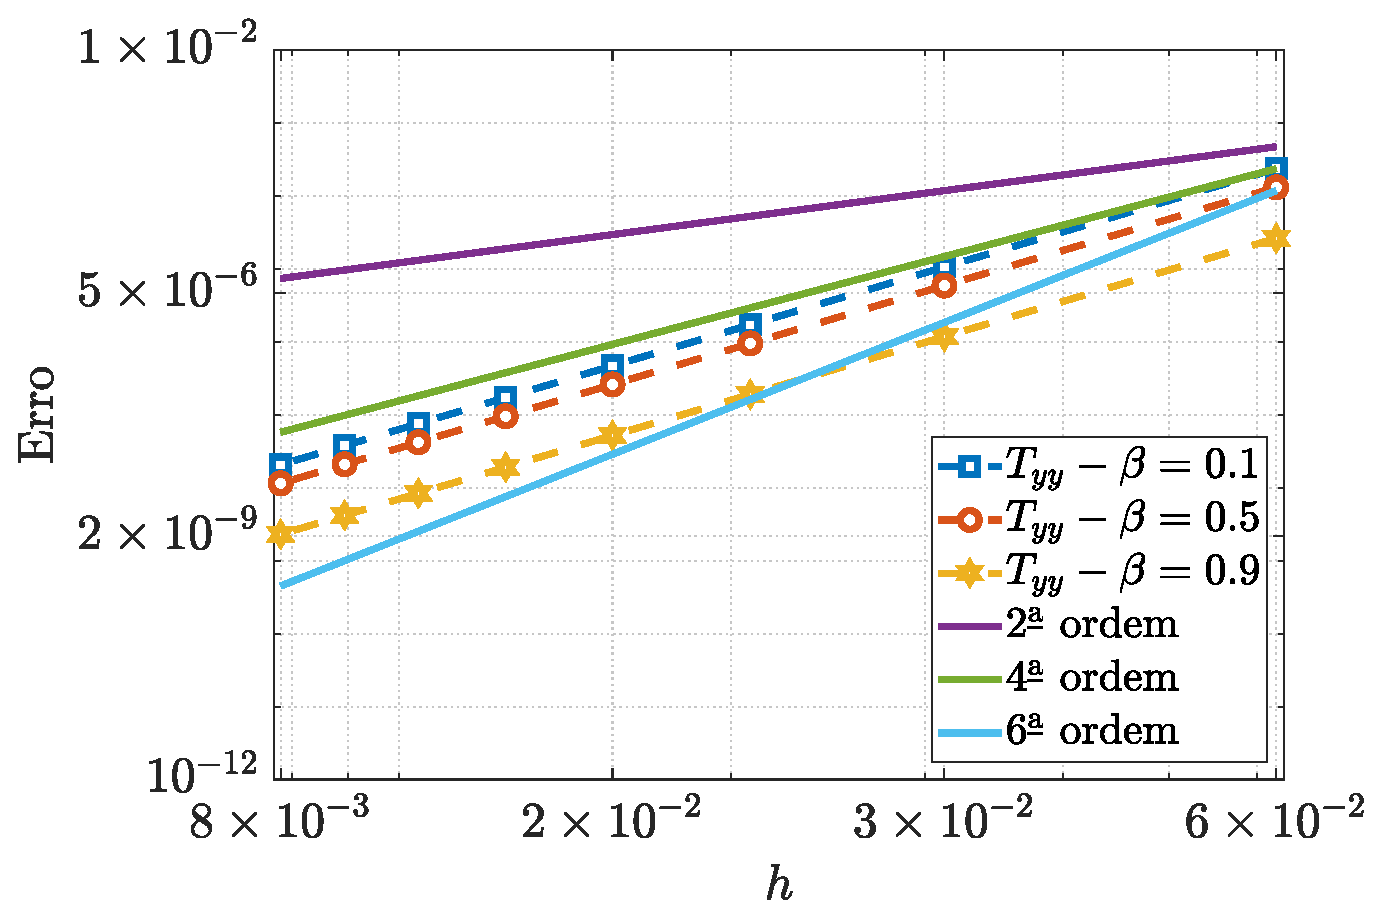
\includegraphics[width=\textwidth]{figures/Case12/Giesekus/Errors/NormErr_2nd_Re_100_Wi_1_epsilon_0_xi_0_alphaG_0.1_Dt_1e-06_at_0.05_tipsim_1_MMS_12_Tyy.eps}
        \caption{$||T_{yy} - \overline{T}_{yy}||_{2}$}
        \label{error_tyy_2nd_Case1_giesekus_alphaG_0.1}
    \end{subfigure}
    \fautor
\end{figure}

\begin{table}[H]
	\IBGEtab{
		\caption{Erros numéricos e cálculo da ordem de convergência para $\omega_{z}$, usando os parâmetros $Wi = 1$ e $\alpha_G = 0.1$, para o fluxo de fluido viscoelástico de Giesekus}\label{tab_GiesekusWzalphaG01Resumida}
	}{
		\begin{tabular*}{\textwidth}{@{\extracolsep\fill}c|c|cc|cc|cc|cc@{}}
                \toprule
                \multirow{2}{*}{$Re$} & \multirow{2}{*}{Malha} & \multicolumn{2}{c}{$\beta_{nn}=0.1$}  & \multicolumn{2}{c}{$\beta_{nn}=0.5$}  & \multicolumn{2}{c}{$\beta_{nn}=0.9$}  & \multicolumn{2}{c}{$\beta_{nn}=1.0$}  \\
                \cline{3-10}
                 & & Erro & p & Erro & p & Erro & p & Erro & p \\
                \midrule
                \multirow{10}{*}{1.00} & 17$\times$17 & 3.02e-03 & --- & 2.77e-03 & --- & 2.57e-03 & --- & 2.52e-03 & --- \\
                & 33$\times$33 & 2.54e-04 & 3.57 & 1.70e-04 & 4.03 & 1.35e-04 & 4.25 & 1.29e-04 & 4.29 \\
                & 49$\times$49 & 4.87e-05 & 4.07 & 2.59e-05 & 4.64 & 1.99e-05 & 4.72 & 1.90e-05 & 4.73 \\
                & 65$\times$65 & 1.32e-05 & 4.53 & 6.41e-06 & 4.85 & 4.91e-06 & 4.86 & 4.68e-06 & 4.86 \\
                & 81$\times$81 & 4.46e-06 & 4.87 & 2.14e-06 & 4.91 & 1.67e-06 & 4.84 & 1.60e-06 & 4.81 \\
                & 97$\times$97 & 1.76e-06 & 5.09 & 8.69e-07 & 4.95 & 6.98e-07 & 4.77 & 6.76e-07 & 4.72 \\
                & 113$\times$113 & 7.91e-07 & 5.20 & 4.11e-07 & 4.86 & 3.46e-07 & 4.55 & 3.38e-07 & 4.50 \\
                & 129$\times$129 & 4.07e-07 & 4.98 & 2.39e-07 & 4.05 & 2.14e-07 & 3.61 & 2.11e-07 & 3.54 \\
                \midrule
                \multirow{10}{*}{100.00} & 17$\times$17 & 3.10e-03 & --- & 3.09e-03 & --- & 3.08e-03 & --- & 3.08e-03 & --- \\
                & 33$\times$33 & 2.93e-04 & 3.40 & 2.91e-04 & 3.41 & 2.88e-04 & 3.42 & 2.88e-04 & 3.42 \\
                & 49$\times$49 & 6.76e-05 & 3.62 & 6.65e-05 & 3.64 & 6.54e-05 & 3.66 & 6.51e-05 & 3.66 \\
                & 65$\times$65 & 2.30e-05 & 3.75 & 2.23e-05 & 3.79 & 2.17e-05 & 3.83 & 2.16e-05 & 3.84 \\
                & 81$\times$81 & 9.72e-06 & 3.86 & 9.28e-06 & 3.93 & 8.88e-06 & 4.01 & 8.79e-06 & 4.02 \\
                & 97$\times$97 & 4.66e-06 & 4.03 & 4.36e-06 & 4.14 & 4.09e-06 & 4.25 & 4.03e-06 & 4.27 \\
                & 113$\times$113 & 2.42e-06 & 4.25 & 2.21e-06 & 4.41 & 2.03e-06 & 4.55 & 1.99e-06 & 4.58 \\
                & 129$\times$129 & 1.38e-06 & 4.22 & 1.22e-06 & 4.46 & 1.09e-06 & 4.67 & 1.06e-06 & 4.71 \\
                \midrule
                \multirow{10}{*}{400.00} & 17$\times$17 & 3.10e-03 & --- & 3.09e-03 & --- & 3.08e-03 & --- & 3.08e-03 & --- \\
                & 33$\times$33 & 2.93e-04 & 3.40 & 2.92e-04 & 3.40 & 2.91e-04 & 3.40 & 2.91e-04 & 3.40 \\
                & 49$\times$49 & 6.78e-05 & 3.61 & 6.74e-05 & 3.62 & 6.71e-05 & 3.62 & 6.70e-05 & 3.62 \\
                & 65$\times$65 & 2.31e-05 & 3.74 & 2.29e-05 & 3.75 & 2.28e-05 & 3.76 & 2.27e-05 & 3.76 \\
                & 81$\times$81 & 9.80e-06 & 3.85 & 9.69e-06 & 3.86 & 9.58e-06 & 3.88 & 9.55e-06 & 3.88 \\
                & 97$\times$97 & 4.72e-06 & 4.01 & 4.64e-06 & 4.04 & 4.57e-06 & 4.06 & 4.55e-06 & 4.06 \\
                & 113$\times$113 & 2.46e-06 & 4.22 & 2.41e-06 & 4.25 & 2.36e-06 & 4.28 & 2.35e-06 & 4.29 \\
                & 129$\times$129 & 1.41e-06 & 4.17 & 1.37e-06 & 4.22 & 1.33e-06 & 4.27 & 1.33e-06 & 4.28 \\
                \midrule
                \multirow{10}{*}{1000.00} & 17$\times$17 & 3.10e-03 & --- & 3.09e-03 & --- & 3.09e-03 & --- & 3.08e-03 & --- \\
                & 33$\times$33 & 2.93e-04 & 3.40 & 2.93e-04 & 3.40 & 2.92e-04 & 3.40 & 2.92e-04 & 3.40 \\
                & 49$\times$49 & 6.78e-05 & 3.61 & 6.76e-05 & 3.61 & 6.74e-05 & 3.61 & 6.74e-05 & 3.61 \\
                & 65$\times$65 & 2.31e-05 & 3.74 & 2.31e-05 & 3.74 & 2.30e-05 & 3.74 & 2.30e-05 & 3.74 \\
                & 81$\times$81 & 9.82e-06 & 3.84 & 9.77e-06 & 3.85 & 9.73e-06 & 3.85 & 9.72e-06 & 3.85 \\
                & 97$\times$97 & 4.73e-06 & 4.00 & 4.70e-06 & 4.01 & 4.68e-06 & 4.02 & 4.67e-06 & 4.02 \\
                & 113$\times$113 & 2.47e-06 & 4.21 & 2.45e-06 & 4.22 & 2.44e-06 & 4.23 & 2.43e-06 & 4.23 \\
                & 129$\times$129 & 1.42e-06 & 4.16 & 1.41e-06 & 4.17 & 1.39e-06 & 4.18 & 1.39e-06 & 4.18 \\
                \bottomrule
            \end{tabular*}
	}{%
		\fdadospesquisa
	}
\end{table}

\begin{table}[H]
	\IBGEtab{
		\caption{Erros numéricos e cálculo da ordem de convergência para a componente do tensor extra-tensões $T_{xy}$, utilizando os parâmetros $Wi=1$ e $\alpha_G = 0.1$, para o escoamento de fluido viscoelástico com o modelo Giesekus}\label{tab_GiesekusTxyalphaG01Resumida}
	}{
            \begin{tabular*}{\textwidth}{@{\extracolsep\fill}c|c|cc|cc|cc|cc@{}}
                \toprule
                \multirow{2}{*}{$Re$} & \multirow{2}{*}{Malha} & \multicolumn{2}{c}{$\beta_{nn}=0.1$}  & \multicolumn{2}{c}{$\beta_{nn}=0.5$}  & \multicolumn{2}{c}{$\beta_{nn}=0.9$}  & \multicolumn{2}{c}{$\beta_{nn}=1.0$}  \\
                \cline{3-10}
                 & & Erro & p & Erro & p & Erro & p & Erro & p \\
                \midrule
                \multirow{10}{*}{1.00} & 17$\times$17 & 2.34e-04 & --- & 1.30e-04 & --- & 2.60e-05 & --- & 2.60e-18 & --- \\
                & 33$\times$33 & 1.06e-05 & 4.46 & 5.90e-06 & 4.46 & 1.18e-06 & 4.46 & 1.18e-19 & 4.46 \\
                & 49$\times$49 & 1.72e-06 & 4.49 & 9.56e-07 & 4.49 & 1.91e-07 & 4.49 & 1.91e-20 & 4.49 \\
                & 65$\times$65 & 4.73e-07 & 4.49 & 2.63e-07 & 4.49 & 5.25e-08 & 4.49 & 5.25e-21 & 4.49 \\
                & 81$\times$81 & 1.73e-07 & 4.50 & 9.63e-08 & 4.49 & 1.93e-08 & 4.49 & 1.93e-21 & 4.49 \\
                & 97$\times$97 & 7.64e-08 & 4.50 & 4.25e-08 & 4.49 & 8.50e-09 & 4.49 & 8.49e-22 & 4.49 \\
                & 113$\times$113 & 3.82e-08 & 4.50 & 2.12e-08 & 4.49 & 4.25e-09 & 4.49 & 4.25e-22 & 4.49 \\
                & 129$\times$129 & 2.10e-08 & 4.50 & 1.17e-08 & 4.49 & 2.33e-09 & 4.49 & 2.33e-22 & 4.49 \\
                \midrule
                \multirow{10}{*}{100.00} & 17$\times$17 & 2.32e-04 & --- & 1.29e-04 & --- & 2.58e-05 & --- & 2.57e-18 & --- \\
                & 33$\times$33 & 1.05e-05 & 4.47 & 5.81e-06 & 4.47 & 1.16e-06 & 4.47 & 1.16e-19 & 4.47 \\
                & 49$\times$49 & 1.69e-06 & 4.49 & 9.40e-07 & 4.49 & 1.88e-07 & 4.49 & 1.88e-20 & 4.49 \\
                & 65$\times$65 & 4.64e-07 & 4.50 & 2.58e-07 & 4.50 & 5.16e-08 & 4.50 & 5.15e-21 & 4.50 \\
                & 81$\times$81 & 1.70e-07 & 4.50 & 9.45e-08 & 4.50 & 1.89e-08 & 4.50 & 1.89e-21 & 4.50 \\
                & 97$\times$97 & 7.49e-08 & 4.50 & 4.16e-08 & 4.50 & 8.33e-09 & 4.50 & 8.32e-22 & 4.50 \\
                & 113$\times$113 & 3.74e-08 & 4.50 & 2.08e-08 & 4.50 & 4.16e-09 & 4.50 & 4.16e-22 & 4.50 \\
                & 129$\times$129 & 2.05e-08 & 4.50 & 1.14e-08 & 4.50 & 2.28e-09 & 4.50 & 2.28e-22 & 4.50 \\
                \midrule
                \multirow{10}{*}{400.00} & 17$\times$17 & 2.27e-04 & --- & 1.26e-04 & --- & 2.53e-05 & --- & 2.52e-18 & --- \\
                & 33$\times$33 & 1.01e-05 & 4.49 & 5.61e-06 & 4.49 & 1.12e-06 & 4.49 & 1.12e-19 & 4.49 \\
                & 49$\times$49 & 1.62e-06 & 4.51 & 9.02e-07 & 4.51 & 1.80e-07 & 4.51 & 1.80e-20 & 4.51 \\
                & 65$\times$65 & 4.44e-07 & 4.51 & 2.47e-07 & 4.51 & 4.93e-08 & 4.51 & 4.93e-21 & 4.51 \\
                & 81$\times$81 & 1.62e-07 & 4.51 & 9.02e-08 & 4.51 & 1.80e-08 & 4.51 & 1.80e-21 & 4.51 \\
                & 97$\times$97 & 7.14e-08 & 4.50 & 3.97e-08 & 4.50 & 7.94e-09 & 4.50 & 7.93e-22 & 4.50 \\
                & 113$\times$113 & 3.57e-08 & 4.50 & 1.98e-08 & 4.50 & 3.97e-09 & 4.50 & 3.96e-22 & 4.50 \\
                & 129$\times$129 & 1.96e-08 & 4.50 & 1.09e-08 & 4.50 & 2.17e-09 & 4.50 & 2.17e-22 & 4.50 \\
                \midrule
                \multirow{10}{*}{1000.00} & 17$\times$17 & 2.22e-04 & --- & 1.23e-04 & --- & 2.46e-05 & --- & 2.46e-18 & --- \\
                & 33$\times$33 & 9.70e-06 & 4.51 & 5.39e-06 & 4.51 & 1.08e-06 & 4.51 & 1.08e-19 & 4.51 \\
                & 49$\times$49 & 1.54e-06 & 4.53 & 8.58e-07 & 4.53 & 1.72e-07 & 4.53 & 1.72e-20 & 4.53 \\
                & 65$\times$65 & 4.20e-07 & 4.52 & 2.34e-07 & 4.52 & 4.67e-08 & 4.52 & 4.67e-21 & 4.52 \\
                & 81$\times$81 & 1.53e-07 & 4.52 & 8.52e-08 & 4.52 & 1.70e-08 & 4.52 & 1.70e-21 & 4.52 \\
                & 97$\times$97 & 6.73e-08 & 4.52 & 3.74e-08 & 4.52 & 7.48e-09 & 4.51 & 7.47e-22 & 4.51 \\
                & 113$\times$113 & 3.36e-08 & 4.51 & 1.87e-08 & 4.51 & 3.73e-09 & 4.51 & 3.73e-22 & 4.51 \\
                & 129$\times$129 & 1.84e-08 & 4.51 & 1.02e-08 & 4.51 & 2.04e-09 & 4.51 & 2.04e-22 & 4.51 \\
                \bottomrule
            \end{tabular*}
	}{%
		\fdadospesquisa
	}
\end{table}

A \autoref{tab_GiesekusWzalphaG01Resumida} e \autoref{tab_GiesekusTxyalphaG01Resumida} apresentam os erros e a ordem de convergência para a vorticidade e o tensor $T_{xy}$, considerando $Wi = 1$ e $\alpha_G = 0.1$. Os resultados obtidos demonstram que, à medida que a malha é refinada, os erros diminuem significativamente, enquanto a ordem de convergência permanece próxima de 4.5. Isso confirma que o esquema numérico é eficiente na captura das propriedades do escoamento, mesmo em malhas mais finas, garantindo uma representação precisa tanto da vorticidade quanto das tensões extras, mesmo em escoamentos de fluidos viscoelásticos com afinamento por cisalhamento.
\begin{figure}[H] 
    \centering 
    \caption{Erro para o campo de velocidade $(\overline{u},\tilde{v})$, vorticidade $(\tilde{\omega_{z}})$, e função de corrente $(\tilde{\psi})$, considerando $Re=100$, $Wi=1$ e $\alpha_G=0.5$, para o escoamento de fluido viscoelástico com o modelo Giesekus}\label{GEerror051}
     \begin{subfigure}[b]{.47\textwidth}
        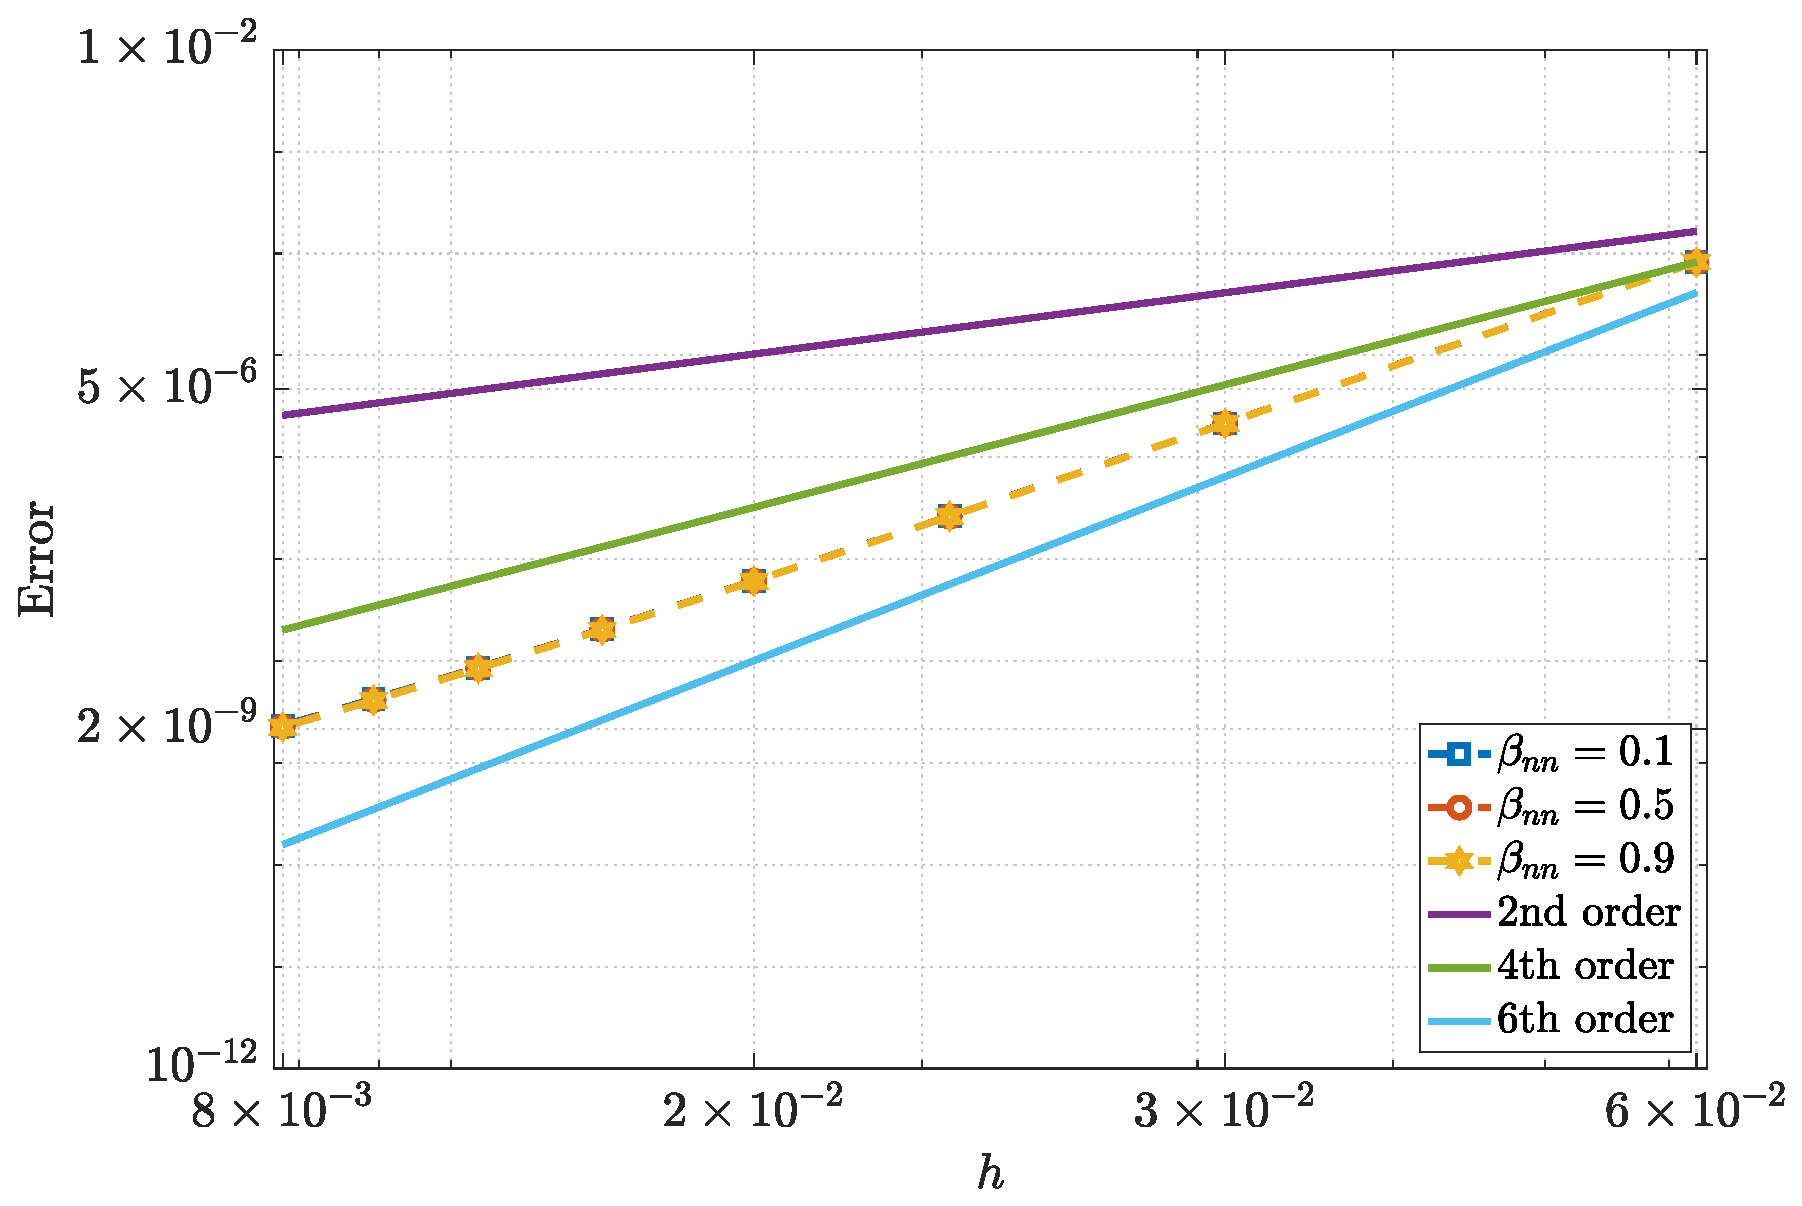
\includegraphics[width=\textwidth]{figures/Case12/Giesekus/Errors/NormErr_2nd_Re_100_Wi_1_epsilon_0_xi_0_alphaG_0.5_Dt_1e-06_at_0.05_tipsim_1_MMS_12_U.eps}
        \caption{$||U - \overline{u}||_{2}$}
        \label{error_u_2nd_Case1_giesekus_alphaG_0.5}
    \end{subfigure}
    \vspace{0.2cm}
    \qquad
    \begin{subfigure}[b]{.47\textwidth}
        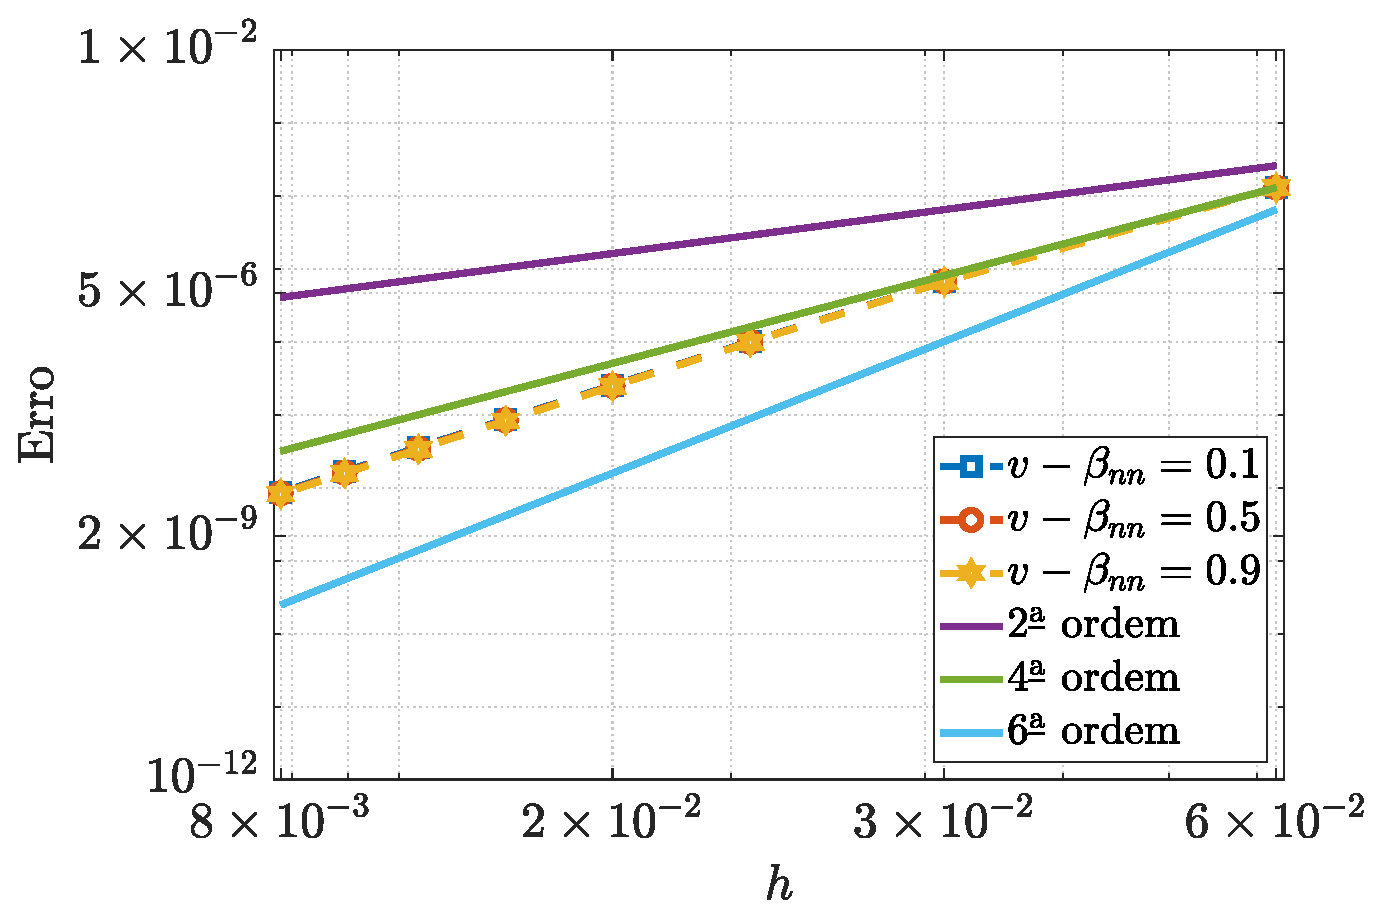
\includegraphics[width=\textwidth]{figures/Case12/Giesekus/Errors/NormErr_2nd_Re_100_Wi_1_epsilon_0_xi_0_alphaG_0.1_Dt_1e-06_at_0.05_tipsim_1_MMS_12_V.eps}
        \caption{$||V - \widetilde{v}||_{2}$}
        \label{error_v_2nd_Case1_giesekus_alphaG_0.5}
    \end{subfigure}
    \qquad
    \begin{subfigure}[b]{.47\textwidth}
        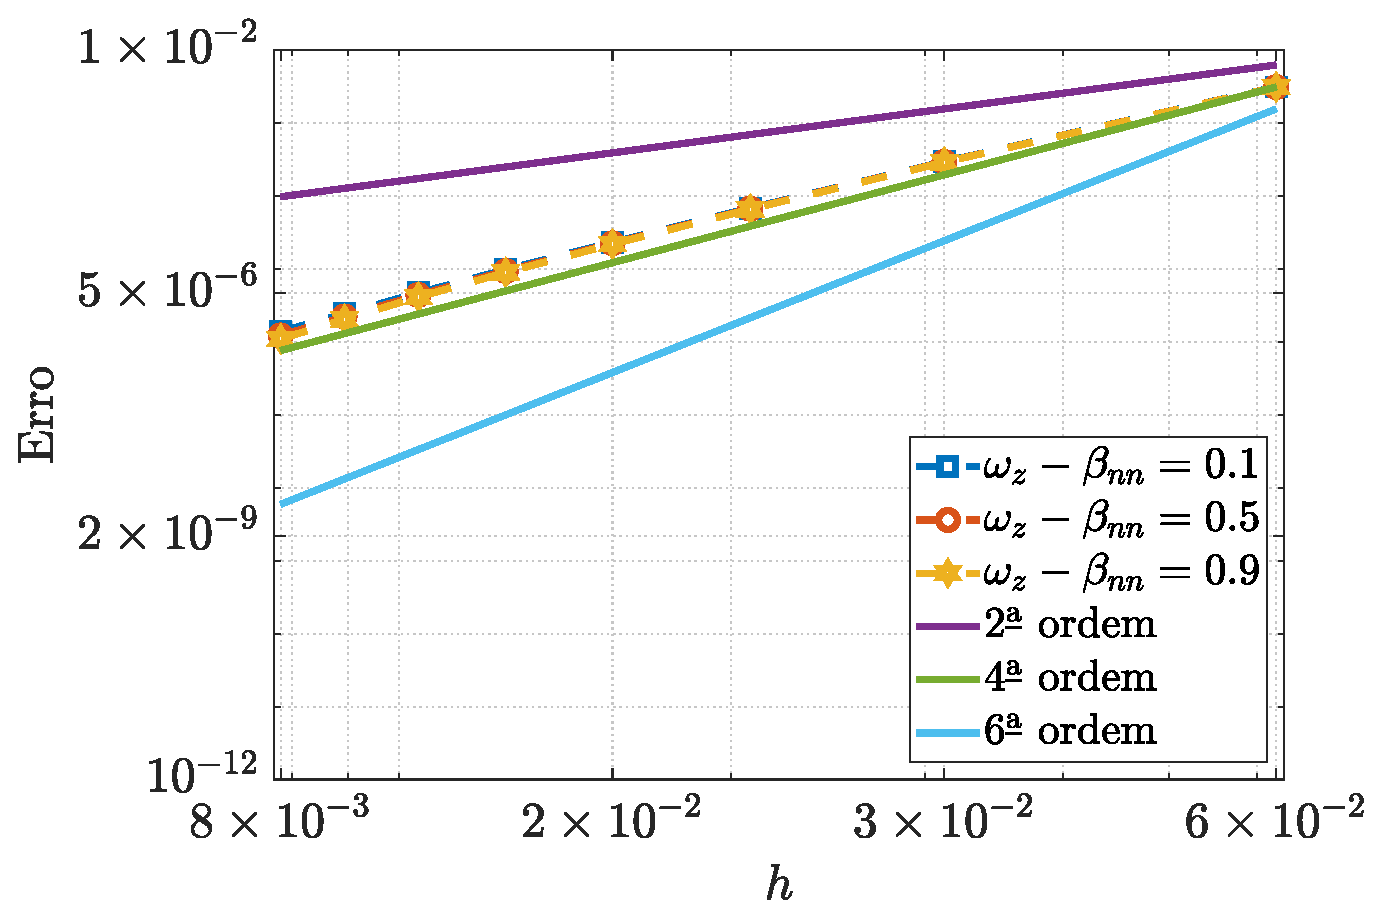
\includegraphics[width=\textwidth]{figures/Case12/Giesekus/Errors/NormErr_2nd_Re_100_Wi_1_epsilon_0_xi_0_alphaG_0.1_Dt_1e-06_at_0.05_tipsim_1_MMS_12_Wz.eps}
        \caption{$||\Omega_{z} - \widetilde{\omega_{z}}||_{2}$}
        \label{error_wz_2nd_Case1_giesekus_alphaG_0.5}
    \end{subfigure}
    \qquad
    \begin{subfigure}[b]{.47\textwidth}
        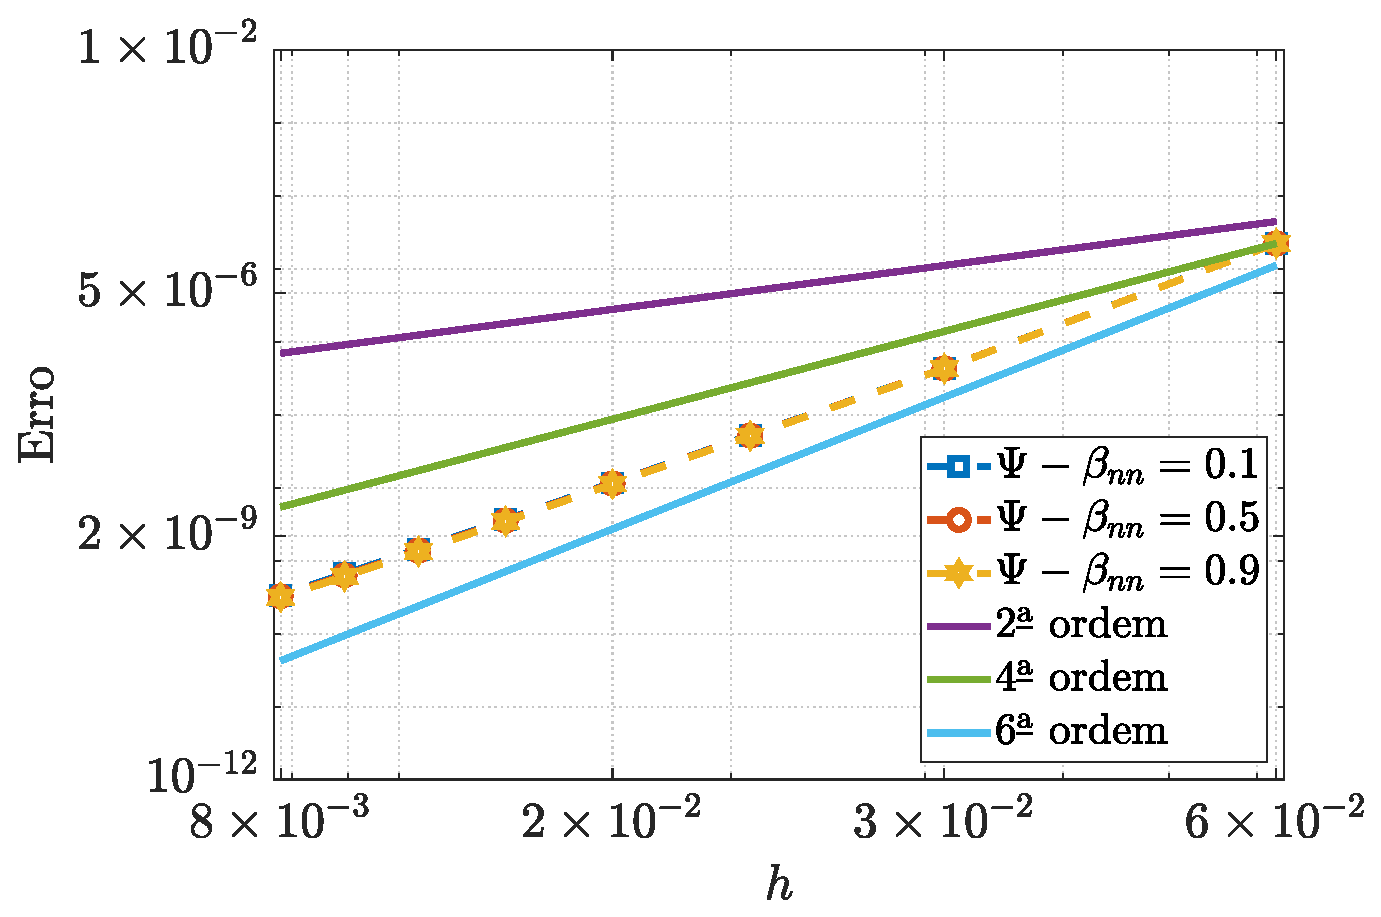
\includegraphics[width=\textwidth]{figures/Case12/Giesekus/Errors/NormErr_2nd_Re_100_Wi_1_epsilon_0_xi_0_alphaG_0.1_Dt_1e-06_at_0.05_tipsim_1_MMS_12_Psi.eps}
        \caption{$||\Psi - \widetilde{\Psi}||_{2}$}
        \label{error_psi_2nd_Case1_oldorydbgiesekus_alphaG_0.5}
    \end{subfigure}
    \fdadospesquisa
\end{figure}

A \autoref{GEerror052} exibe gráficos de erros representando os componentes do tensor extra-tensões, para o escoamento de fluido viscoelástico com o modelo Giesekus com $Re=100$, $Wi=1$ e $\alpha_G=0.5$.
\begin{figure}[H] 
    \centering
    \caption{Erro para os componentes dos tensores extra-tensões, utilizando os parâmetros $Re=100,$ $Wi=1$ e $\alpha_{G} = 0.5$, para o escoamento de fluido viscoelástico Giesekus}\label{GEerror052}
    \begin{subfigure}[b]{.47\textwidth}
        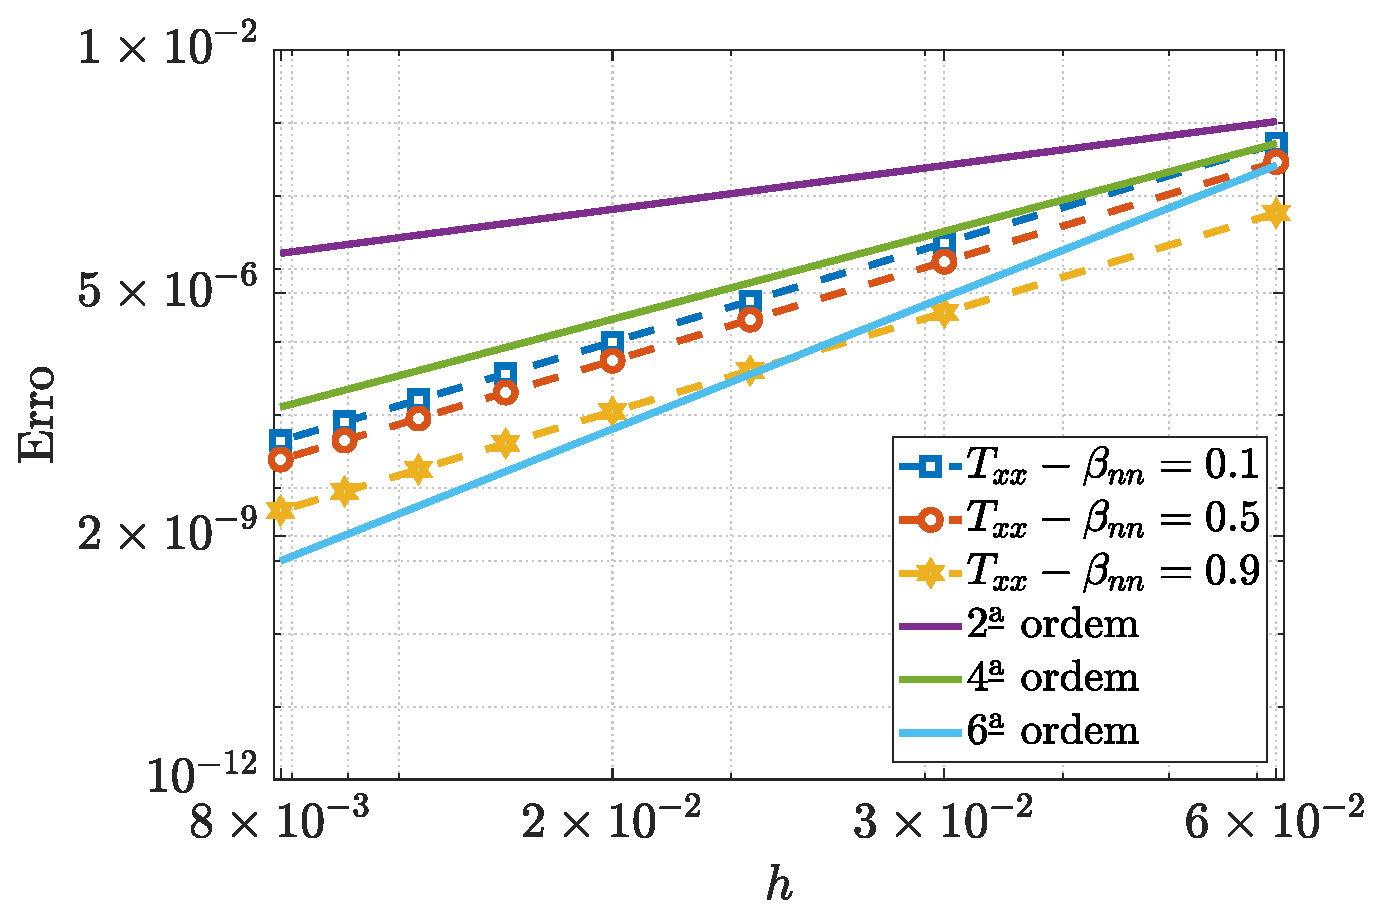
\includegraphics[width=\textwidth]{figures/Case12/Giesekus/Errors/NormErr_2nd_Re_100_Wi_1_epsilon_0_xi_0_alphaG_0.1_Dt_1e-06_at_0.05_tipsim_1_MMS_12_Txx.eps}
        \caption{$||T_{xx} - \overline{T}_{xx}||_{2}$}
        \label{error_txx_2nd_Case1_giesekus_alphaG_0.5}
    \end{subfigure}
    \vspace{0.2cm}
    \qquad
    \begin{subfigure}[b]{.47\textwidth}
        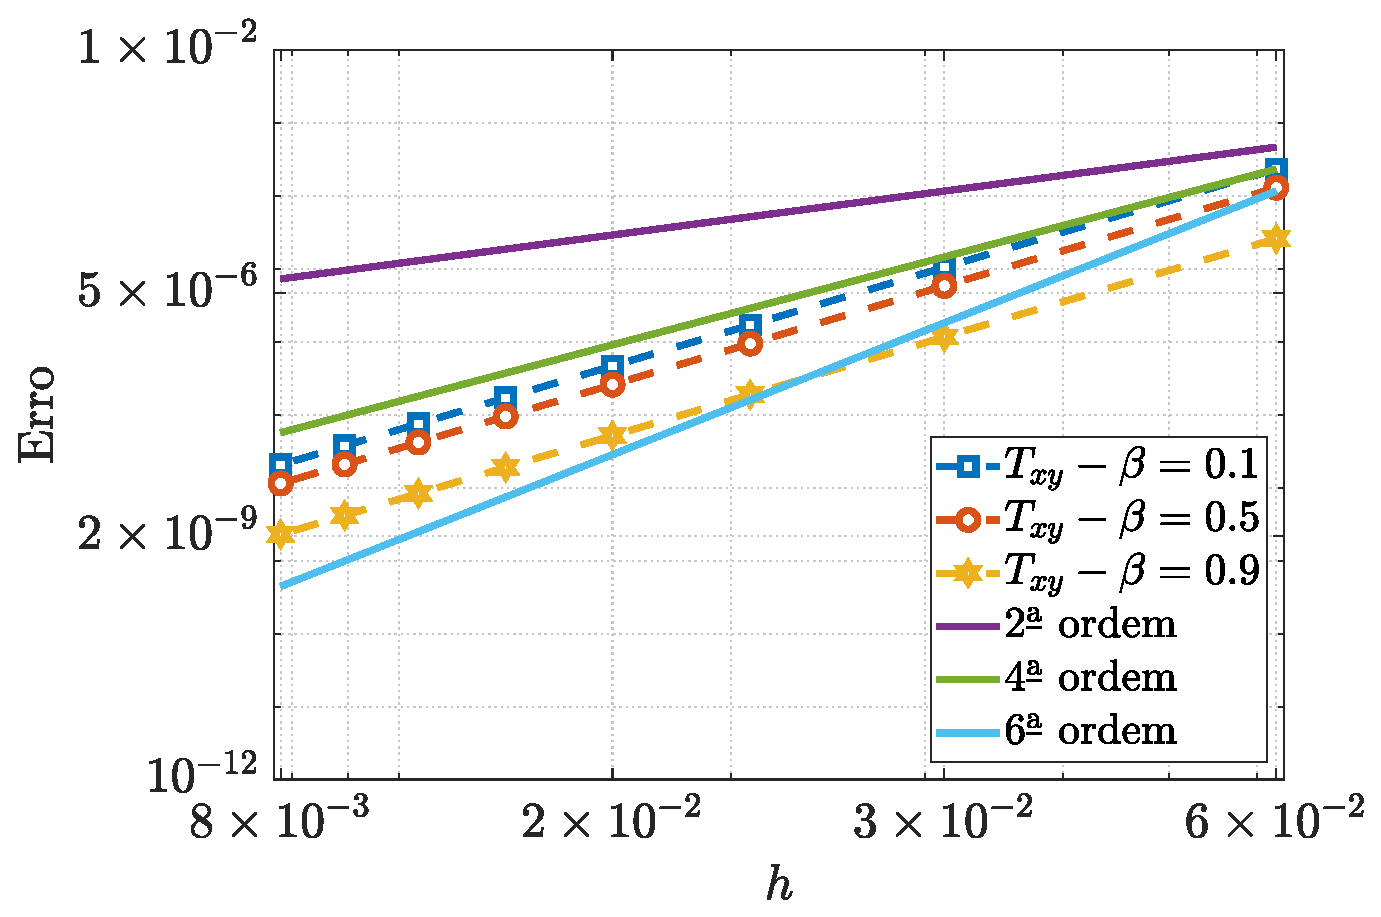
\includegraphics[width=\textwidth]{figures/Case12/Giesekus/Errors/NormErr_2nd_Re_100_Wi_1_epsilon_0_xi_0_alphaG_0.1_Dt_1e-06_at_0.05_tipsim_1_MMS_12_Txy.eps}
        \caption{$||T_{xy} - \overline{T}_{xy}||_{2}$}
        \label{error_txy_2nd_Case1_giesekus_alphaG_0.5}
    \end{subfigure}
    \qquad
    \begin{subfigure}[b]{.47\textwidth}
        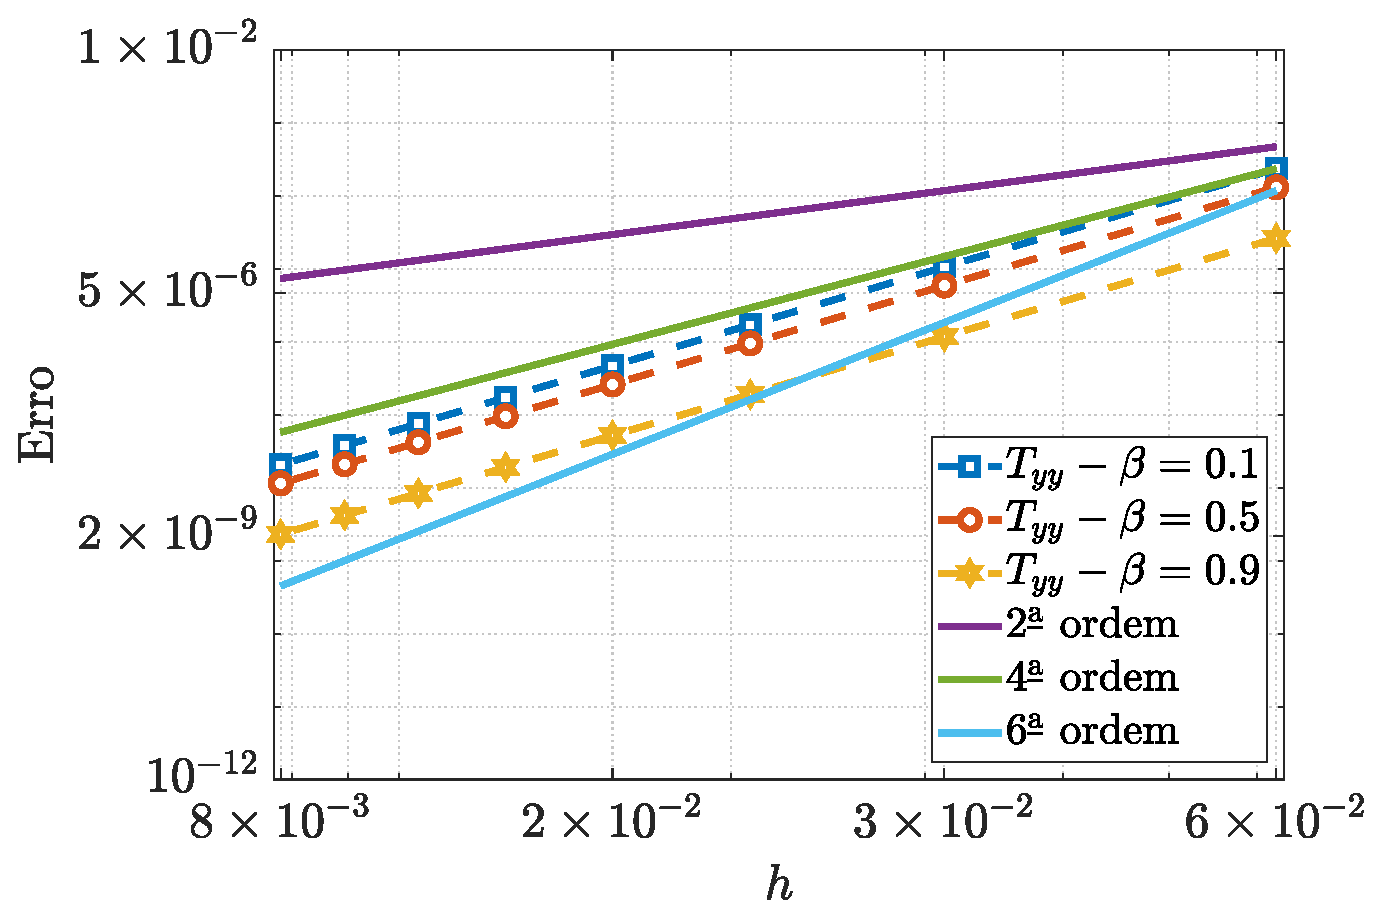
\includegraphics[width=\textwidth]{figures/Case12/Giesekus/Errors/NormErr_2nd_Re_100_Wi_1_epsilon_0_xi_0_alphaG_0.1_Dt_1e-06_at_0.05_tipsim_1_MMS_12_Tyy.eps}
        \caption{$||T_{yy} - \overline{T}_{yy}||_{2}$}
        \label{error_tyy_2nd_Case1_giesekus_alphaG_0.5}
    \end{subfigure}
    \fautor
\end{figure}

Nas simulações com $\alpha_G = 0.5$, apresentadas nas Figuras \ref{GEerror051} e \ref{GEerror052}, observa-se uma similaridade nos resultados em comparação com aqueles obtidos com $\alpha_G = 0.1$. A ordem de convergência permanece consistente, aproximando-se de 4.5 para todas as variáveis estudadas, incluindo os tensores de tensões e a vorticidade. Isso indica que o modelo de Giesekus é estável e preciso em uma ampla gama de valores de $\alpha_G$, tornando-o aplicável em diversas condições de escoamento. Além disso, a precisão do modelo é mantida mesmo com o aumento do parâmetro $\alpha_G$, sugerindo que o esquema numérico implementado é robusto o suficiente para simular diferentes regimes de viscosidade e elasticidade em fluidos viscoelásticos.
\begin{table}[H]
	\IBGEtab{
		\caption{Erros numéricos e cálculo da ordem de convergência para o componente do tensor de tensões $T_{yy}$, utilizando os parâmetros $Wi = 1$ e $\alpha_G = 0.1$, para o escoamento de fluido viscoelástico de Giesekus}\label{tab:GiesekusWzalphaG05Resumida}
	}{
            \begin{tabular*}{\textwidth}{@{\extracolsep\fill}c|c|cc|cc|cc|cc@{}}
                \toprule
                \multirow{2}{*}{$Re$} & \multirow{2}{*}{Malha} & \multicolumn{2}{c}{$\beta_{nn}=0.1$}  & \multicolumn{2}{c}{$\beta_{nn}=0.5$}  & \multicolumn{2}{c}{$\beta_{nn}=0.9$}  & \multicolumn{2}{c}{$\beta_{nn}=1.0$}  \\
                \cline{3-10}
                 & & Erro & p & Erro & p & Erro & p & Erro & p \\
                \midrule
                \multirow{10}{*}{1.00} & 17$\times$17 & 2.34e-04 & --- & 1.30e-04 & --- & 2.60e-05 & --- & 2.60e-18 & --- \\
                & 33$\times$33 & 1.06e-05 & 4.46 & 5.90e-06 & 4.46 & 1.18e-06 & 4.46 & 1.18e-19 & 4.46 \\
                & 49$\times$49 & 1.72e-06 & 4.49 & 9.56e-07 & 4.49 & 1.91e-07 & 4.49 & 1.91e-20 & 4.49 \\
                & 65$\times$65 & 4.72e-07 & 4.49 & 2.62e-07 & 4.49 & 5.25e-08 & 4.49 & 5.25e-21 & 4.49 \\
                & 81$\times$81 & 1.73e-07 & 4.50 & 9.62e-08 & 4.50 & 1.93e-08 & 4.50 & 1.92e-21 & 4.50 \\
                & 97$\times$97 & 7.63e-08 & 4.50 & 4.24e-08 & 4.50 & 8.48e-09 & 4.50 & 8.47e-22 & 4.50 \\
                & 113$\times$113 & 3.81e-08 & 4.50 & 2.12e-08 & 4.50 & 4.24e-09 & 4.50 & 4.24e-22 & 4.50 \\
                & 129$\times$129 & 2.09e-08 & 4.50 & 1.16e-08 & 4.50 & 2.33e-09 & 4.50 & 2.32e-22 & 4.50 \\
                \midrule
                \multirow{10}{*}{100.00} & 17$\times$17 & 2.35e-04 & --- & 1.31e-04 & --- & 2.61e-05 & --- & 2.61e-18 & --- \\
                & 33$\times$33 & 1.06e-05 & 4.48 & 5.86e-06 & 4.48 & 1.17e-06 & 4.48 & 1.17e-19 & 4.48 \\
                & 49$\times$49 & 1.70e-06 & 4.50 & 9.46e-07 & 4.50 & 1.89e-07 & 4.50 & 1.89e-20 & 4.50 \\
                & 65$\times$65 & 4.67e-07 & 4.50 & 2.59e-07 & 4.50 & 5.19e-08 & 4.50 & 5.18e-21 & 4.50 \\
                & 81$\times$81 & 1.71e-07 & 4.50 & 9.50e-08 & 4.50 & 1.90e-08 & 4.50 & 1.90e-21 & 4.50 \\
                & 97$\times$97 & 7.52e-08 & 4.50 & 4.18e-08 & 4.50 & 8.36e-09 & 4.50 & 8.36e-22 & 4.50 \\
                & 113$\times$113 & 3.76e-08 & 4.50 & 2.09e-08 & 4.50 & 4.18e-09 & 4.50 & 4.18e-22 & 4.50 \\
                & 129$\times$129 & 2.06e-08 & 4.50 & 1.15e-08 & 4.50 & 2.29e-09 & 4.50 & 2.29e-22 & 4.50 \\
                \midrule
                \multirow{10}{*}{400.00} & 17$\times$17 & 2.37e-04 & --- & 1.32e-04 & --- & 2.63e-05 & --- & 2.63e-18 & --- \\
                & 33$\times$33 & 1.04e-05 & 4.51 & 5.78e-06 & 4.51 & 1.16e-06 & 4.51 & 1.16e-19 & 4.51 \\
                & 49$\times$49 & 1.66e-06 & 4.52 & 9.24e-07 & 4.52 & 1.85e-07 & 4.52 & 1.85e-20 & 4.52 \\
                & 65$\times$65 & 4.54e-07 & 4.52 & 2.52e-07 & 4.52 & 5.04e-08 & 4.52 & 5.04e-21 & 4.52 \\
                & 81$\times$81 & 1.66e-07 & 4.51 & 9.21e-08 & 4.51 & 1.84e-08 & 4.51 & 1.84e-21 & 4.51 \\
                & 97$\times$97 & 7.28e-08 & 4.51 & 4.04e-08 & 4.51 & 8.09e-09 & 4.51 & 8.08e-22 & 4.51 \\
                & 113$\times$113 & 3.63e-08 & 4.51 & 2.02e-08 & 4.51 & 4.04e-09 & 4.51 & 4.03e-22 & 4.51 \\
                & 129$\times$129 & 1.99e-08 & 4.51 & 1.11e-08 & 4.51 & 2.21e-09 & 4.51 & 2.21e-22 & 4.51 \\
                \midrule
                \multirow{10}{*}{1000.00} & 17$\times$17 & 2.43e-04 & --- & 1.35e-04 & --- & 2.70e-05 & --- & 2.70e-18 & --- \\
                & 33$\times$33 & 1.03e-05 & 4.56 & 5.73e-06 & 4.56 & 1.15e-06 & 4.56 & 1.14e-19 & 4.56 \\
                & 49$\times$49 & 1.62e-06 & 4.56 & 9.02e-07 & 4.56 & 1.80e-07 & 4.56 & 1.80e-20 & 4.56 \\
                & 65$\times$65 & 4.39e-07 & 4.54 & 2.44e-07 & 4.54 & 4.88e-08 & 4.54 & 4.88e-21 & 4.54 \\
                & 81$\times$81 & 1.60e-07 & 4.53 & 8.88e-08 & 4.53 & 1.78e-08 & 4.53 & 1.77e-21 & 4.53 \\
                & 97$\times$97 & 7.00e-08 & 4.53 & 3.89e-08 & 4.53 & 7.78e-09 & 4.53 & 7.77e-22 & 4.53 \\
                & 113$\times$113 & 3.48e-08 & 4.52 & 1.94e-08 & 4.52 & 3.87e-09 & 4.52 & 3.87e-22 & 4.52 \\
                & 129$\times$129 & 1.91e-08 & 4.52 & 1.06e-08 & 4.52 & 2.12e-09 & 4.52 & 2.12e-22 & 4.52 \\
                \bottomrule
            \end{tabular*}
	}{%
	\fdadospesquisa
	}
\end{table}

\begin{table}[H]
	\IBGEtab{
	   \caption{Erros numéricos e cálculo da ordem de convergência para o componente do tensor de tensões $T_{yy}$, utilizando os parâmetros $Wi = 1$ e $\alpha_G = 0.5$, para o escoamento de fluido viscoelástico de Giesekus}\label{tab:GiesekusTyyalphaG05Resumida}
	}{
            \begin{tabular*}{\textwidth}{@{\extracolsep\fill}c|c|cc|cc|cc|cc@{}}
                \toprule
                \multirow{2}{*}{$Re$} & \multirow{2}{*}{Malha} & \multicolumn{2}{c}{$\beta_{nn}=0.1$}  & \multicolumn{2}{c}{$\beta_{nn}=0.5$}  & \multicolumn{2}{c}{$\beta_{nn}=0.9$}  & \multicolumn{2}{c}{$\beta_{nn}=1.0$}  \\
                \cline{3-10}
                 & & Erro & p & Erro & p & Erro & p & Erro & p \\
                \midrule
                \multirow{10}{*}{1.00} & 17$\times$17 & 2.34e-04 & --- & 1.30e-04 & --- & 2.60e-05 & --- & 2.60e-18 & --- \\
                & 33$\times$33 & 1.06e-05 & 4.46 & 5.90e-06 & 4.46 & 1.18e-06 & 4.46 & 1.18e-19 & 4.46 \\
                & 49$\times$49 & 1.72e-06 & 4.49 & 9.56e-07 & 4.49 & 1.91e-07 & 4.49 & 1.91e-20 & 4.49 \\
                & 65$\times$65 & 4.72e-07 & 4.49 & 2.62e-07 & 4.49 & 5.25e-08 & 4.49 & 5.24e-21 & 4.49 \\
                & 81$\times$81 & 1.73e-07 & 4.50 & 9.62e-08 & 4.50 & 1.92e-08 & 4.50 & 1.92e-21 & 4.50 \\
                & 97$\times$97 & 7.62e-08 & 4.50 & 4.24e-08 & 4.50 & 8.48e-09 & 4.50 & 8.47e-22 & 4.50 \\
                & 113$\times$113 & 3.81e-08 & 4.50 & 2.12e-08 & 4.50 & 4.24e-09 & 4.50 & 4.23e-22 & 4.50 \\
                & 129$\times$129 & 2.09e-08 & 4.50 & 1.16e-08 & 4.50 & 2.32e-09 & 4.50 & 2.32e-22 & 4.50 \\
                \midrule
                \multirow{10}{*}{100.00} & 17$\times$17 & 2.38e-04 & --- & 1.32e-04 & --- & 2.64e-05 & --- & 2.64e-18 & --- \\
                & 33$\times$33 & 1.04e-05 & 4.52 & 5.76e-06 & 4.52 & 1.15e-06 & 4.52 & 1.15e-19 & 4.52 \\
                & 49$\times$49 & 1.65e-06 & 4.53 & 9.19e-07 & 4.53 & 1.84e-07 & 4.53 & 1.84e-20 & 4.53 \\
                & 65$\times$65 & 4.50e-07 & 4.52 & 2.50e-07 & 4.52 & 5.00e-08 & 4.52 & 5.00e-21 & 4.52 \\
                & 81$\times$81 & 1.64e-07 & 4.52 & 9.13e-08 & 4.52 & 1.83e-08 & 4.52 & 1.83e-21 & 4.52 \\
                & 97$\times$97 & 7.22e-08 & 4.51 & 4.01e-08 & 4.51 & 8.02e-09 & 4.51 & 8.01e-22 & 4.51 \\
                & 113$\times$113 & 3.60e-08 & 4.51 & 2.00e-08 & 4.51 & 4.00e-09 & 4.51 & 4.00e-22 & 4.51 \\
                & 129$\times$129 & 1.97e-08 & 4.51 & 1.10e-08 & 4.51 & 2.19e-09 & 4.51 & 2.19e-22 & 4.51 \\
                \midrule
                \multirow{10}{*}{400.00} & 17$\times$17 & 2.56e-04 & --- & 1.42e-04 & --- & 2.84e-05 & --- & 2.84e-18 & --- \\
                & 33$\times$33 & 1.04e-05 & 4.61 & 5.80e-06 & 4.61 & 1.16e-06 & 4.61 & 1.16e-19 & 4.61 \\
                & 49$\times$49 & 1.61e-06 & 4.60 & 8.97e-07 & 4.60 & 1.79e-07 & 4.60 & 1.79e-20 & 4.60 \\
                & 65$\times$65 & 4.33e-07 & 4.58 & 2.40e-07 & 4.58 & 4.81e-08 & 4.58 & 4.80e-21 & 4.58 \\
                & 81$\times$81 & 1.56e-07 & 4.56 & 8.69e-08 & 4.56 & 1.74e-08 & 4.56 & 1.74e-21 & 4.56 \\
                & 97$\times$97 & 6.83e-08 & 4.55 & 3.79e-08 & 4.55 & 7.58e-09 & 4.55 & 7.58e-22 & 4.55 \\
                & 113$\times$113 & 3.39e-08 & 4.54 & 1.88e-08 & 4.54 & 3.77e-09 & 4.54 & 3.76e-22 & 4.54 \\
                & 129$\times$129 & 1.85e-08 & 4.54 & 1.03e-08 & 4.53 & 2.06e-09 & 4.53 & 2.05e-22 & 4.53 \\
                \midrule
                \multirow{10}{*}{1000.00} & 17$\times$17 & 3.11e-04 & --- & 1.73e-04 & --- & 3.46e-05 & --- & 3.46e-18 & --- \\
                & 33$\times$33 & 1.17e-05 & 4.74 & 6.47e-06 & 4.74 & 1.29e-06 & 4.74 & 1.29e-19 & 4.74 \\
                & 49$\times$49 & 1.72e-06 & 4.72 & 9.56e-07 & 4.72 & 1.91e-07 & 4.72 & 1.91e-20 & 4.72 \\
                & 65$\times$65 & 4.50e-07 & 4.66 & 2.50e-07 & 4.66 & 5.00e-08 & 4.66 & 5.00e-21 & 4.66 \\
                & 81$\times$81 & 1.60e-07 & 4.62 & 8.91e-08 & 4.62 & 1.78e-08 & 4.62 & 1.78e-21 & 4.62 \\
                & 97$\times$97 & 6.93e-08 & 4.60 & 3.85e-08 & 4.60 & 7.71e-09 & 4.60 & 7.70e-22 & 4.60 \\
                & 113$\times$113 & 3.42e-08 & 4.58 & 1.90e-08 & 4.58 & 3.80e-09 & 4.58 & 3.80e-22 & 4.58 \\
                & 129$\times$129 & 1.86e-08 & 4.57 & 1.03e-08 & 4.57 & 2.06e-09 & 4.57 & 2.06e-22 & 4.57 \\
                \bottomrule
            \end{tabular*}
	}{
		\fdadospesquisa
	}
\end{table}

\subsection{Caso de verificação usando o modelo LPTT}

As simulações numéricas realizadas para verificar o código de alta ordem desenvolvido para escoamentos de fluidos viscoelásticos foram configuradas utilizando o modelo LPTT (Linear Phan-Thien-Tanner), com números de Reynolds variando entre $Re = 1,\ 100,\ 400$ e $1000$, número de Weissenberg $Wi = 1,\ 5$ e $10$. Além disso, a razão de viscosidade do solvente foi definida como $\beta_{nn} = 0.1,\ 0.5,\ 0.9$ e $1.0$, e os parâmetros adicionais de elasticidade e afinamento por cisalhamento ($\epsilon$ e $\xi$) variaram entre $0.5$ e $1.0$ para $\epsilon$, e $0.1$ e $0.5$ para $\xi$, com o objetivo de avaliar o desempenho do modelo em diferentes regimes de escoamento viscoelástico.

A \autoref{LPTTerror1} apresenta os gráficos de erro para os componentes do campo de velocidade, vorticidade e função de corrente, enquanto a \autoref{LPTTerror2} complementa essa análise mostrando os erros associados aos tensores de tensão extra no escoamento de fluido viscoelástico LPTT. Esses gráficos mostram a evolução dos erros para $Re = 100$, $Wi = 1$, e $\beta_{nn} = 0.1,\ 0.5$ e  $0.9$. Vale destacar que os resultados para $\beta_{nn} = 1$ foram omitidos, pois os erros correspondentes estavam na ordem de $10^{-18}$, o que teria distorcido a visualização comparativa dos outros valores de $\beta_{nn}$.
\begin{figure}[H] 
    \centering 
    \caption{Erro para o campo de velocidade $(\overline{u},\tilde{v})$, vorticidade $(\tilde{\omega_{z}})$, e função de corrente $(\tilde{\psi})$, considerando $Re=100$, $Wi=1$, $\epsilon = 0.5$ e $\xi = 0.1$, para o escoamento de fluido viscoelástico com o modelo LPTT}\label{LPTTerror1}
     \begin{subfigure}[b]{.47\textwidth}
        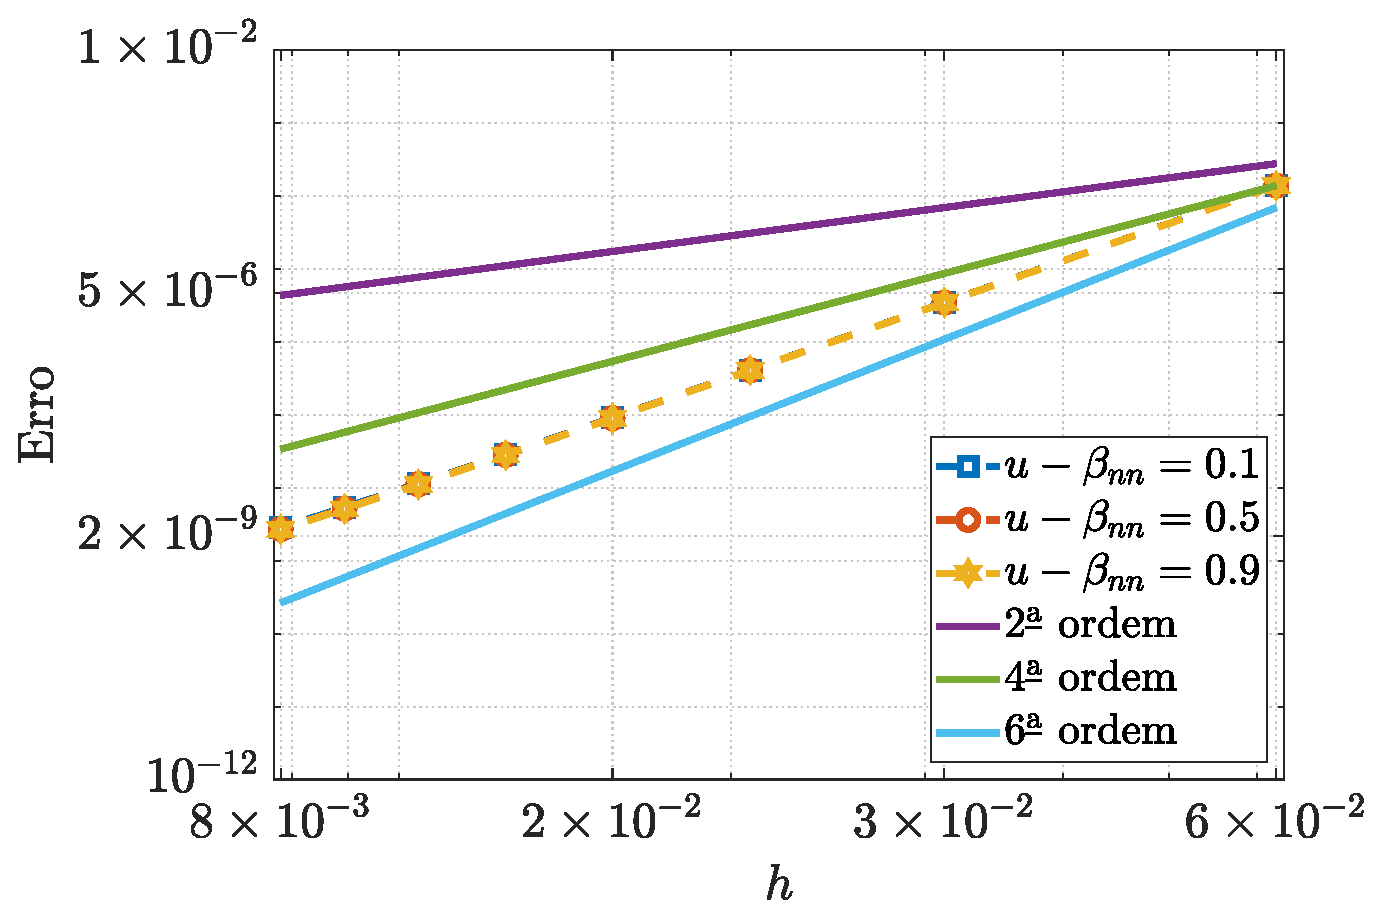
\includegraphics[width=\textwidth]{figures/Case12/LPTT/Errors/NormErr_2nd_Re_100_Wi_1_epsilon_0.5_xi_0.1_alphaG_0_Dt_1e-06_at_0.05_tipsim_1_MMS_12_U.eps}
        \caption{$||U - \overline{u}||_{2}$}
        \label{error_u_2nd_Case1_LPTT_eps_05}
    \end{subfigure}
    \vspace{0.2cm}
    \qquad
    \begin{subfigure}[b]{.47\textwidth}
        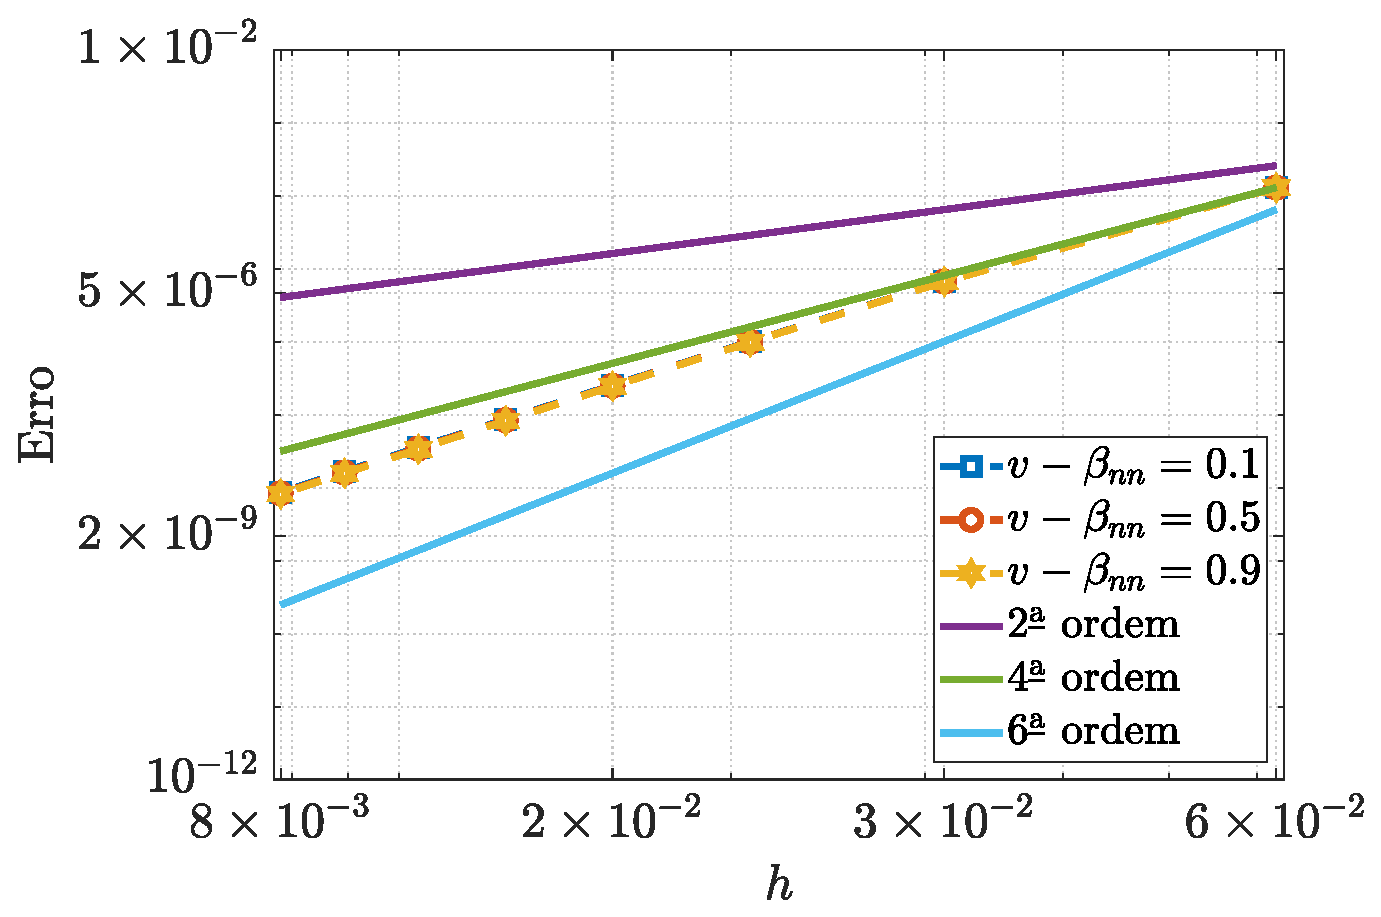
\includegraphics[width=\textwidth]{figures/Case12/LPTT/Errors/NormErr_2nd_Re_100_Wi_1_epsilon_0.5_xi_0.1_alphaG_0_Dt_1e-06_at_0.05_tipsim_1_MMS_12_V.eps}
        \caption{$||V - \widetilde{v}||_{2}$}
        \label{error_v_2nd_Case1_LPTT_eps_05}
    \end{subfigure}
    \qquad
    \begin{subfigure}[b]{.47\textwidth}
        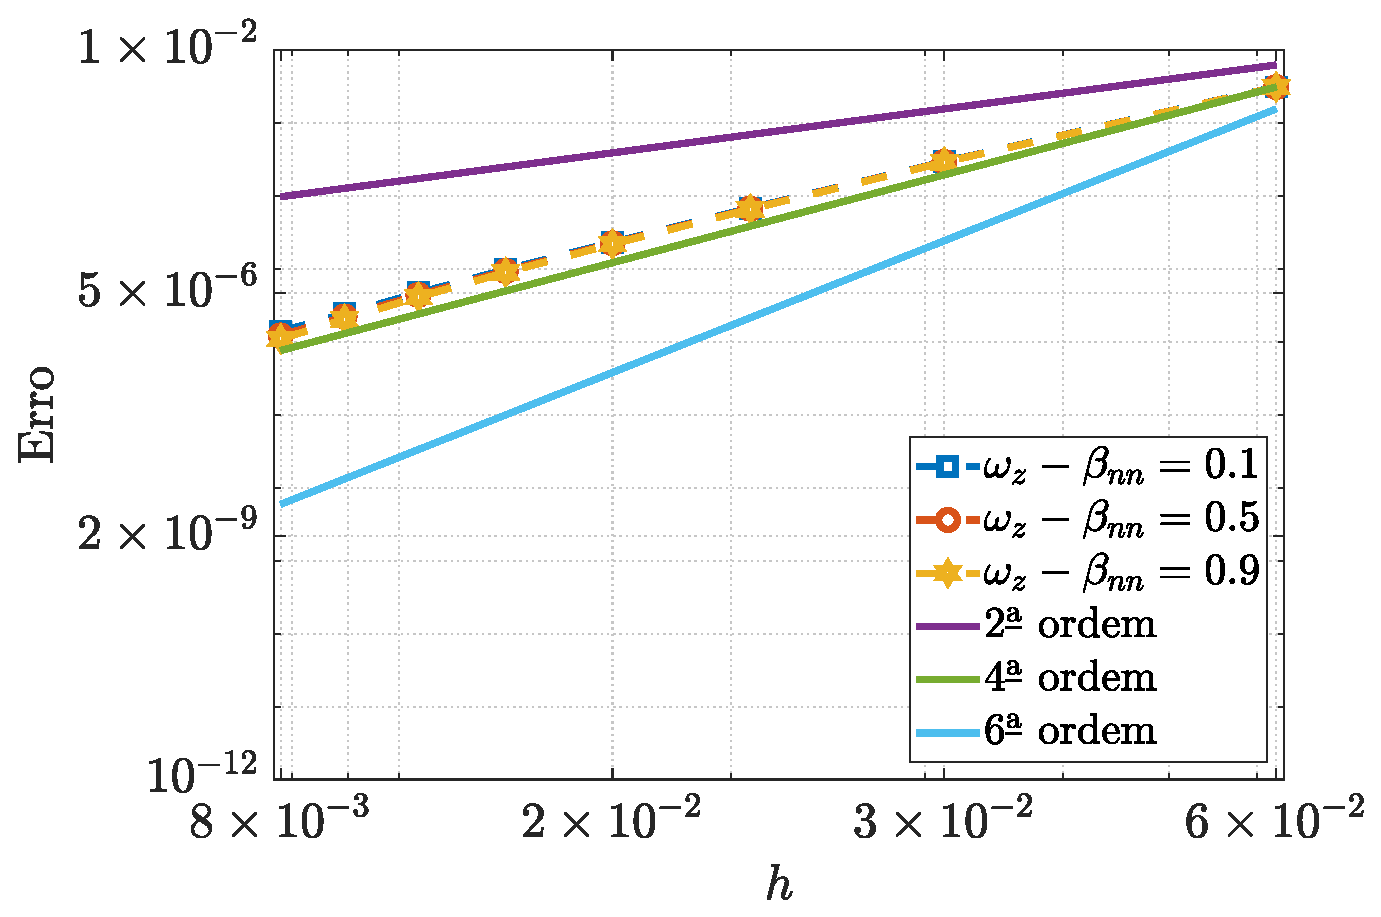
\includegraphics[width=\textwidth]{figures/Case12/LPTT/Errors/NormErr_2nd_Re_100_Wi_1_epsilon_0.5_xi_0.1_alphaG_0_Dt_1e-06_at_0.05_tipsim_1_MMS_12_Wz.eps}
        \caption{$||\Omega_{z} - \widetilde{\omega_{z}}||_{2}$}
        \label{error_wz_2nd_Case1_LPTT_eps_05}
    \end{subfigure}
    \qquad
    \begin{subfigure}[b]{.47\textwidth}
        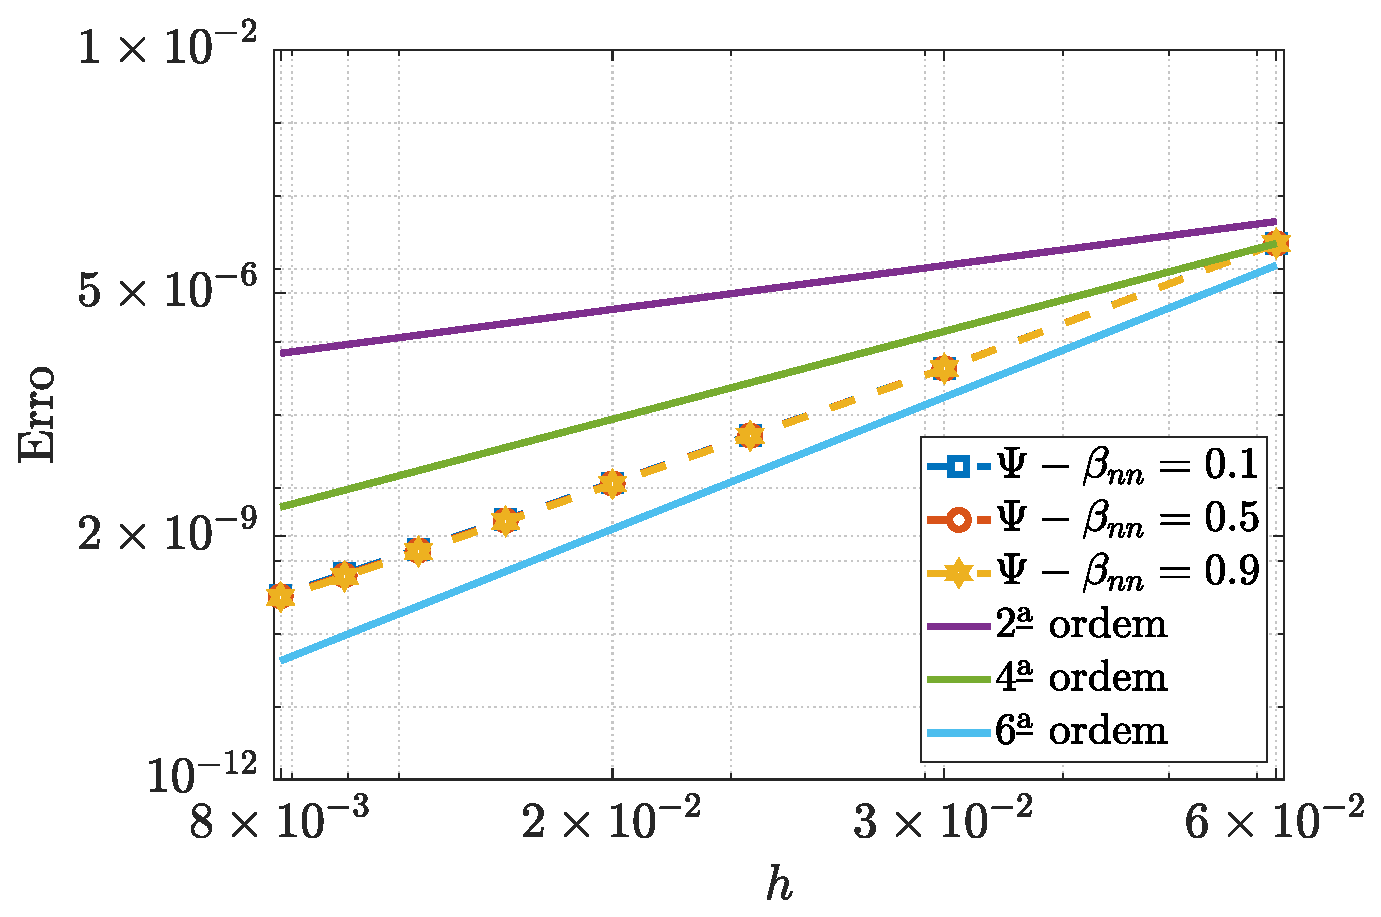
\includegraphics[width=\textwidth]{figures/Case12/LPTT/Errors/NormErr_2nd_Re_100_Wi_1_epsilon_0.5_xi_0.1_alphaG_0_Dt_1e-06_at_0.05_tipsim_1_MMS_12_Psi.eps}
        \caption{$||\Psi - \widetilde{\Psi}||_{2}$}
        \label{error_psi_2nd_Case1_LPTT_eps_05}
    \end{subfigure}
    \fdadospesquisa
\end{figure}

A \autoref{LPTTerror2} exibe gráficos de erros representando os componentes do tensor extra-tensões, para o escoamento de fluido viscoelástico com o modelo LPTT com $Re=100$, $Wi=1$, $\epsilon = 0.5$ e $\xi = 0.1$.
\begin{figure}[H] 
    \centering
    \caption{Erro para os componentes dos tensores extra-tensões, utilizando os parâmetros $Re=100$, $Wi=1$, $\epsilon=0.5$ e $\xi=0.1$, para o escoamento de fluido viscoelástico LPTT}\label{LPTTerror2}
    \begin{subfigure}[b]{.47\textwidth}
        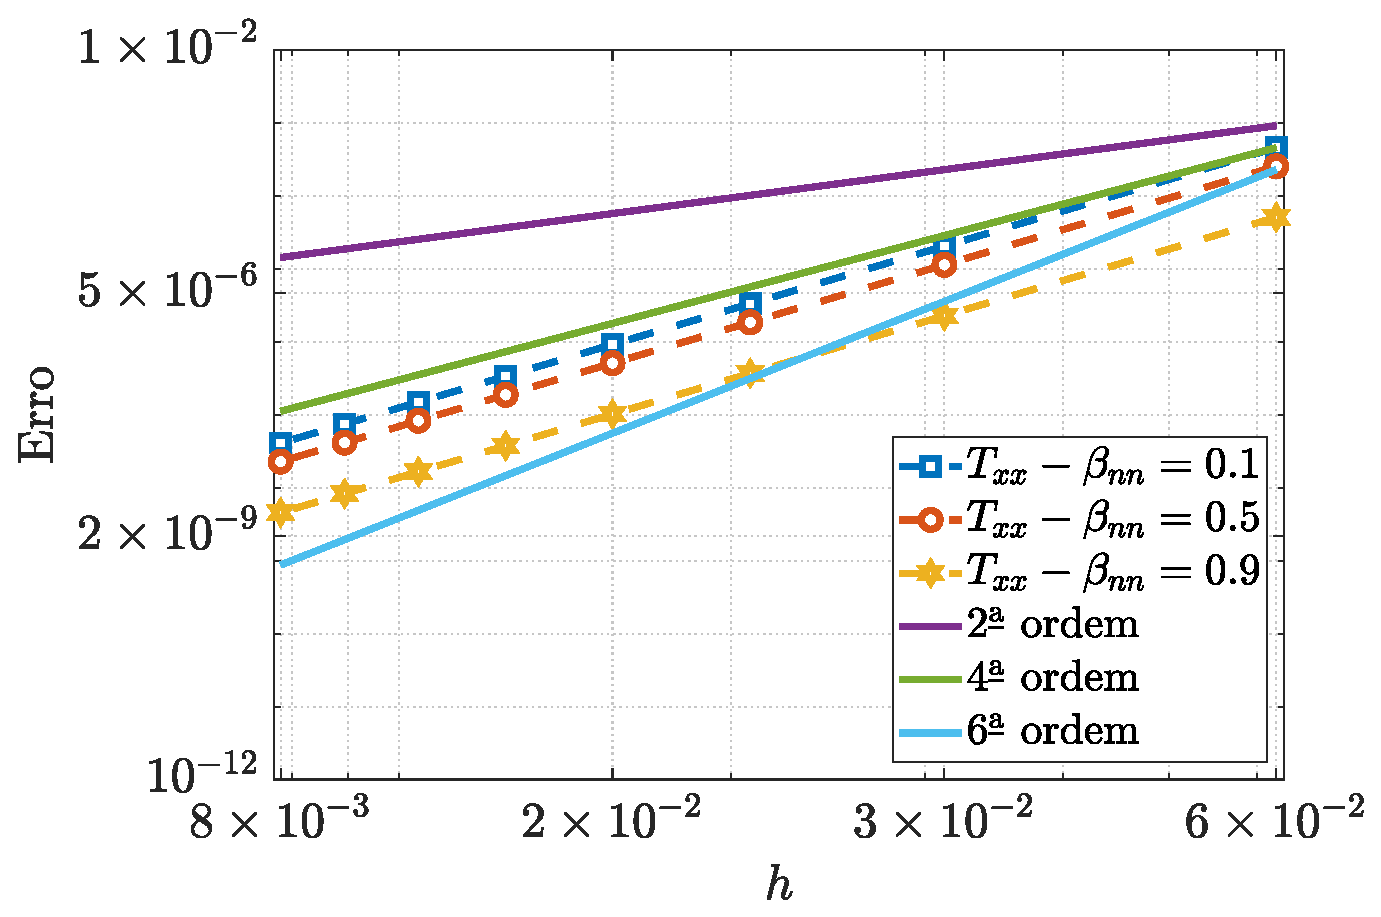
\includegraphics[width=\textwidth]{figures/Case12/LPTT/Errors/NormErr_2nd_Re_100_Wi_1_epsilon_0.5_xi_0.1_alphaG_0_Dt_1e-06_at_0.05_tipsim_1_MMS_12_Txx.eps}
        \caption{$||T_{xx} - \overline{T}_{xx}||_{2}$}
        \label{error_txx_2nd_Case1_LPTT_eps_05}
    \end{subfigure}
    \vspace{0.2cm}
    \qquad
    \begin{subfigure}[b]{.47\textwidth}
        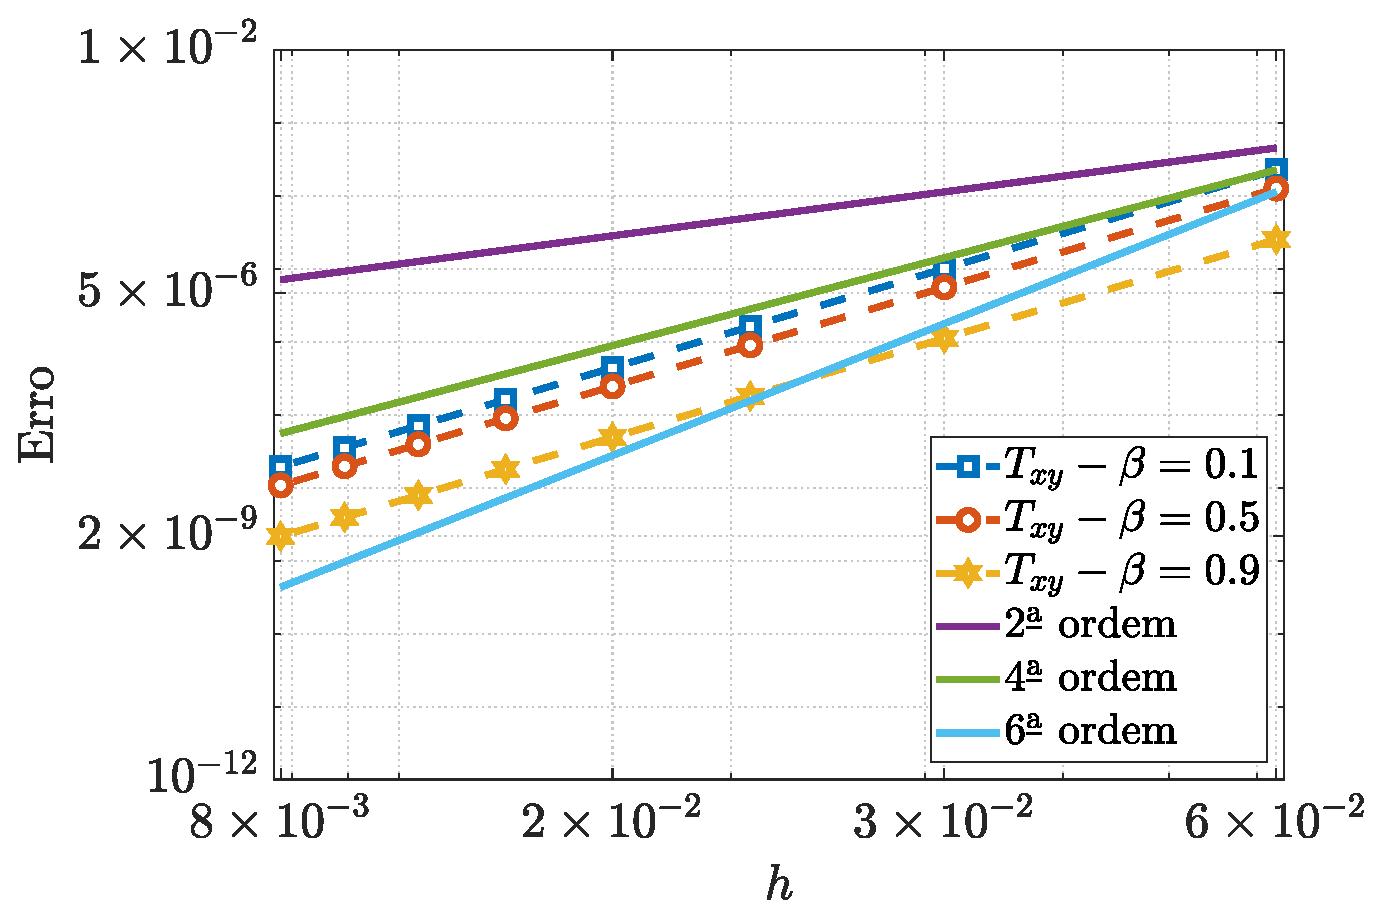
\includegraphics[width=\textwidth]{figures/Case12/LPTT/Errors/NormErr_2nd_Re_100_Wi_1_epsilon_0.5_xi_0.1_alphaG_0_Dt_1e-06_at_0.05_tipsim_1_MMS_12_Txy.eps}
        \caption{$||T_{xy} - \overline{T}_{xy}||_{2}$}
        \label{error_txy_2nd_Case1_LPTT_eps_05}
    \end{subfigure}
    \qquad
    \begin{subfigure}[b]{.47\textwidth}
        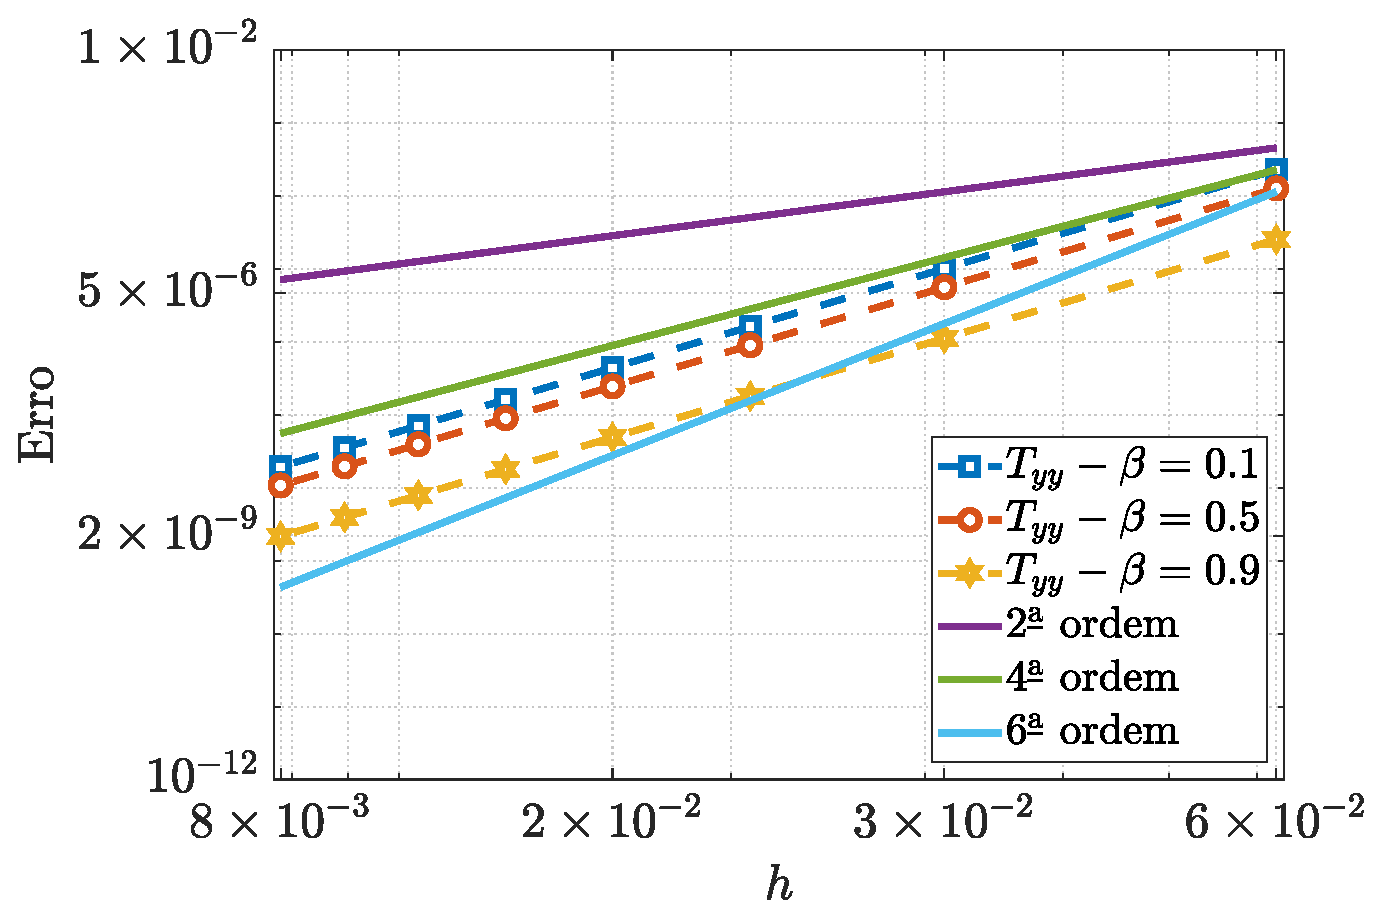
\includegraphics[width=\textwidth]{figures/Case12/LPTT/Errors/NormErr_2nd_Re_100_Wi_1_epsilon_0.5_xi_0.1_alphaG_0_Dt_1e-06_at_0.05_tipsim_1_MMS_12_Tyy.eps}
        \caption{$||T_{yy} - \overline{T}_{yy}||_{2}$}
        \label{error_tyy_2nd_Case1_LPTT_eps_05}
    \end{subfigure}
    \fautor
\end{figure}

A Tabela~\ref{tab_LPTTWzResumida} apresenta os resultados obtidos para a vorticidade $\omega_z$ no contexto do modelo viscoelástico LPTT, considerando os parâmetros fixos $Wi = 1$, $\epsilon = 0.5$ e $\xi = 0.1$. Foram analisadas diversas razões de viscosidade do solvente ($\beta_{nn}$) sob diferentes números de Reynolds ($Re$). A análise numérica avalia os erros absolutos e as ordens de convergência associadas ao refinamento da malha, permitindo verificar a consistência da discretização e a acurácia do esquema adotado para esta variável.

\begin{table}[H]
	\IBGEtab{
		\caption{Erros numéricos e cálculo da ordem de convergência para $\omega_{z}$, usando os parâmetros $Wi=1$, $\epsilon = 0.5$ e $\xi = 0.1$, para o fluxo de fluido viscoelástico de LPTT}\label{tab_LPTTWzResumida}
	}{
		\begin{tabular*}{\textwidth}{@{\extracolsep\fill}c|c|cc|cc|cc|cc@{}}
                \toprule
                \multirow{2}{*}{$Re$} & \multirow{2}{*}{Malha} & \multicolumn{2}{c}{$\beta_{nn}=0.1$}  & \multicolumn{2}{c}{$\beta_{nn}=0.5$}  & \multicolumn{2}{c}{$\beta_{nn}=0.9$}  & \multicolumn{2}{c}{$\beta_{nn}=1.0$}  \\
                \cline{3-10}
                 & & Erro & p & Erro & p & Erro & p & Erro & p \\
                \midrule
                \multirow{10}{*}{1.00} & 17$\times$17 & 3.02e-03 & --- & 2.77e-03 & --- & 2.57e-03 & --- & 2.52e-03 & --- \\
                & 33$\times$33 & 2.54e-04 & 3.57 & 1.70e-04 & 4.03 & 1.35e-04 & 4.25 & 1.29e-04 & 4.29 \\
                & 49$\times$49 & 4.87e-05 & 4.07 & 2.59e-05 & 4.64 & 1.99e-05 & 4.72 & 1.90e-05 & 4.73 \\
                & 65$\times$65 & 1.32e-05 & 4.53 & 6.41e-06 & 4.85 & 4.91e-06 & 4.86 & 4.68e-06 & 4.86 \\
                & 81$\times$81 & 4.46e-06 & 4.87 & 2.14e-06 & 4.91 & 1.67e-06 & 4.84 & 1.60e-06 & 4.81 \\
                & 97$\times$97 & 1.76e-06 & 5.09 & 8.69e-07 & 4.95 & 6.98e-07 & 4.77 & 6.76e-07 & 4.72 \\
                & 113$\times$113 & 7.91e-07 & 5.20 & 4.11e-07 & 4.86 & 3.46e-07 & 4.55 & 3.38e-07 & 4.50 \\
                & 129$\times$129 & 4.07e-07 & 4.98 & 2.39e-07 & 4.05 & 2.14e-07 & 3.61 & 2.11e-07 & 3.54 \\
                \midrule
                \multirow{10}{*}{100.00} & 17$\times$17 & 3.10e-03 & --- & 3.09e-03 & --- & 3.08e-03 & --- & 3.08e-03 & --- \\
                & 33$\times$33 & 2.93e-04 & 3.40 & 2.91e-04 & 3.41 & 2.88e-04 & 3.42 & 2.88e-04 & 3.42 \\
                & 49$\times$49 & 6.76e-05 & 3.62 & 6.65e-05 & 3.64 & 6.54e-05 & 3.66 & 6.51e-05 & 3.66 \\
                & 65$\times$65 & 2.30e-05 & 3.75 & 2.23e-05 & 3.79 & 2.17e-05 & 3.83 & 2.16e-05 & 3.84 \\
                & 81$\times$81 & 9.72e-06 & 3.86 & 9.28e-06 & 3.93 & 8.88e-06 & 4.01 & 8.79e-06 & 4.02 \\
                & 97$\times$97 & 4.66e-06 & 4.03 & 4.36e-06 & 4.14 & 4.09e-06 & 4.25 & 4.03e-06 & 4.27 \\
                & 113$\times$113 & 2.42e-06 & 4.25 & 2.21e-06 & 4.41 & 2.03e-06 & 4.55 & 1.99e-06 & 4.58 \\
                & 129$\times$129 & 1.38e-06 & 4.22 & 1.22e-06 & 4.46 & 1.09e-06 & 4.67 & 1.06e-06 & 4.71 \\
                \midrule
                \multirow{10}{*}{400.00} & 17$\times$17 & 3.10e-03 & --- & 3.09e-03 & --- & 3.08e-03 & --- & 3.08e-03 & --- \\
                & 33$\times$33 & 2.93e-04 & 3.40 & 2.92e-04 & 3.40 & 2.91e-04 & 3.40 & 2.91e-04 & 3.40 \\
                & 49$\times$49 & 6.78e-05 & 3.61 & 6.74e-05 & 3.62 & 6.71e-05 & 3.62 & 6.70e-05 & 3.62 \\
                & 65$\times$65 & 2.31e-05 & 3.74 & 2.29e-05 & 3.75 & 2.28e-05 & 3.76 & 2.27e-05 & 3.76 \\
                & 81$\times$81 & 9.81e-06 & 3.84 & 9.69e-06 & 3.86 & 9.58e-06 & 3.88 & 9.55e-06 & 3.88 \\
                & 97$\times$97 & 4.72e-06 & 4.01 & 4.64e-06 & 4.03 & 4.57e-06 & 4.06 & 4.55e-06 & 4.06 \\
                & 113$\times$113 & 2.47e-06 & 4.21 & 2.41e-06 & 4.25 & 2.36e-06 & 4.28 & 2.35e-06 & 4.29 \\
                & 129$\times$129 & 1.42e-06 & 4.16 & 1.37e-06 & 4.22 & 1.33e-06 & 4.27 & 1.33e-06 & 4.28 \\
                \midrule
                \multirow{10}{*}{1000.00} & 17$\times$17 & 3.10e-03 & --- & 3.09e-03 & --- & 3.09e-03 & --- & 3.08e-03 & --- \\
                & 33$\times$33 & 2.93e-04 & 3.40 & 2.93e-04 & 3.40 & 2.92e-04 & 3.40 & 2.92e-04 & 3.40 \\
                & 49$\times$49 & 6.78e-05 & 3.61 & 6.76e-05 & 3.61 & 6.74e-05 & 3.61 & 6.74e-05 & 3.61 \\
                & 65$\times$65 & 2.32e-05 & 3.73 & 2.31e-05 & 3.74 & 2.30e-05 & 3.74 & 2.30e-05 & 3.74 \\
                & 81$\times$81 & 9.84e-06 & 3.84 & 9.78e-06 & 3.85 & 9.73e-06 & 3.85 & 9.72e-06 & 3.85 \\
                & 97$\times$97 & 4.75e-06 & 4.00 & 4.71e-06 & 4.01 & 4.68e-06 & 4.02 & 4.67e-06 & 4.02 \\
                & 113$\times$113 & 2.49e-06 & 4.19 & 2.46e-06 & 4.21 & 2.44e-06 & 4.23 & 2.43e-06 & 4.23 \\
                & 129$\times$129 & 1.43e-06 & 4.13 & 1.41e-06 & 4.16 & 1.39e-06 & 4.18 & 1.39e-06 & 4.18 \\
                \bottomrule
            \end{tabular*}
	}{%
	\fdadospesquisa
	}
\end{table}

Na Tabela~\ref{tab_LPTTTxxResumida}, são apresentados os resultados referentes ao componente $T_{xx}$ do tensor de tensões extra. As simulações foram realizadas sob as mesmas condições utilizadas anteriormente ($Wi = 1$, $\epsilon = 0.5$, $\xi = 0.1$), variando-se os valores de $\beta_{nn}$ e $Re$.
\begin{table}[H]
	\IBGEtab{
		\caption{Erros numéricos e cálculo da ordem de convergência para a componente do tensor extra-tensões $T_{xx}$, usando os parâmetros $Wi=1$, $\epsilon = 0.5$ e $\xi = 0.1$, para o fluxo de fluido viscoelástico de LPTT}\label{tab_LPTTTxxResumida}
	}{
            \begin{tabular*}{\textwidth}{@{\extracolsep\fill}c|c|cc|cc|cc|cc@{}}
                \toprule
                \multirow{2}{*}{$Re$} & \multirow{2}{*}{Malha} & \multicolumn{2}{c}{$\beta_{nn}=0.1$}  & \multicolumn{2}{c}{$\beta_{nn}=0.5$}  & \multicolumn{2}{c}{$\beta_{nn}=0.9$}  & \multicolumn{2}{c}{$\beta_{nn}=1.0$}  \\
                \cline{3-10}
                 & & Erro & p & Erro & p & Erro & p & Erro & p \\
                \midrule
                \multirow{10}{*}{1.00} & 17$\times$17 & 5.37e-04 & --- & 2.98e-04 & --- & 5.96e-05 & --- & 5.96e-18 & --- \\
                & 33$\times$33 & 2.30e-05 & 4.54 & 1.28e-05 & 4.54 & 2.56e-06 & 4.54 & 2.55e-19 & 4.54 \\
                & 49$\times$49 & 3.69e-06 & 4.52 & 2.05e-06 & 4.52 & 4.10e-07 & 4.52 & 4.09e-20 & 4.52 \\
                & 65$\times$65 & 1.01e-06 & 4.51 & 5.60e-07 & 4.51 & 1.12e-07 & 4.51 & 1.12e-20 & 4.51 \\
                & 81$\times$81 & 3.69e-07 & 4.50 & 2.05e-07 & 4.50 & 4.10e-08 & 4.50 & 4.09e-21 & 4.50 \\
                & 97$\times$97 & 1.62e-07 & 4.50 & 9.02e-08 & 4.50 & 1.80e-08 & 4.50 & 1.80e-21 & 4.50 \\
                & 113$\times$113 & 8.11e-08 & 4.50 & 4.50e-08 & 4.50 & 9.01e-09 & 4.50 & 9.00e-22 & 4.50 \\
                & 129$\times$129 & 4.44e-08 & 4.50 & 2.47e-08 & 4.50 & 4.94e-09 & 4.50 & 4.93e-22 & 4.50 \\
                \midrule
                \multirow{10}{*}{100.00} & 17$\times$17 & 4.56e-04 & --- & 2.53e-04 & --- & 5.07e-05 & --- & 5.06e-18 & --- \\
                & 33$\times$33 & 2.04e-05 & 4.49 & 1.13e-05 & 4.49 & 2.26e-06 & 4.49 & 2.26e-19 & 4.49 \\
                & 49$\times$49 & 3.32e-06 & 4.47 & 1.84e-06 & 4.47 & 3.68e-07 & 4.47 & 3.68e-20 & 4.47 \\
                & 65$\times$65 & 9.14e-07 & 4.48 & 5.08e-07 & 4.48 & 1.02e-07 & 4.48 & 1.02e-20 & 4.48 \\
                & 81$\times$81 & 3.36e-07 & 4.48 & 1.87e-07 & 4.48 & 3.74e-08 & 4.48 & 3.73e-21 & 4.48 \\
                & 97$\times$97 & 1.48e-07 & 4.48 & 8.25e-08 & 4.48 & 1.65e-08 & 4.48 & 1.65e-21 & 4.48 \\
                & 113$\times$113 & 7.44e-08 & 4.49 & 4.13e-08 & 4.49 & 8.26e-09 & 4.49 & 8.26e-22 & 4.49 \\
                & 129$\times$129 & 4.08e-08 & 4.49 & 2.27e-08 & 4.49 & 4.54e-09 & 4.49 & 4.53e-22 & 4.49 \\
                \midrule
                \multirow{10}{*}{400.00} & 17$\times$17 & 3.36e-04 & --- & 1.87e-04 & --- & 3.73e-05 & --- & 3.73e-18 & --- \\
                & 33$\times$33 & 1.64e-05 & 4.35 & 9.14e-06 & 4.35 & 1.83e-06 & 4.35 & 1.83e-19 & 4.35 \\
                & 49$\times$49 & 2.78e-06 & 4.38 & 1.54e-06 & 4.38 & 3.09e-07 & 4.38 & 3.09e-20 & 4.38 \\
                & 65$\times$65 & 7.81e-07 & 4.41 & 4.34e-07 & 4.41 & 8.68e-08 & 4.41 & 8.67e-21 & 4.41 \\
                & 81$\times$81 & 2.91e-07 & 4.43 & 1.61e-07 & 4.43 & 3.23e-08 & 4.43 & 3.23e-21 & 4.43 \\
                & 97$\times$97 & 1.29e-07 & 4.44 & 7.18e-08 & 4.44 & 1.44e-08 & 4.44 & 1.43e-21 & 4.44 \\
                & 113$\times$113 & 6.51e-08 & 4.45 & 3.61e-08 & 4.45 & 7.23e-09 & 4.45 & 7.22e-22 & 4.45 \\
                & 129$\times$129 & 3.59e-08 & 4.46 & 1.99e-08 & 4.46 & 3.99e-09 & 4.46 & 3.98e-22 & 4.46 \\
                \midrule
                \multirow{10}{*}{1000.00} & 17$\times$17 & 2.59e-04 & --- & 1.44e-04 & --- & 2.88e-05 & --- & 2.88e-18 & --- \\
                & 33$\times$33 & 1.35e-05 & 4.26 & 7.53e-06 & 4.26 & 1.51e-06 & 4.26 & 1.50e-19 & 4.26 \\
                & 49$\times$49 & 2.39e-06 & 4.28 & 1.33e-06 & 4.28 & 2.65e-07 & 4.28 & 2.65e-20 & 4.28 \\
                & 65$\times$65 & 6.85e-07 & 4.34 & 3.81e-07 & 4.34 & 7.61e-08 & 4.34 & 7.61e-21 & 4.34 \\
                & 81$\times$81 & 2.58e-07 & 4.37 & 1.44e-07 & 4.37 & 2.87e-08 & 4.37 & 2.87e-21 & 4.37 \\
                & 97$\times$97 & 1.16e-07 & 4.39 & 6.45e-08 & 4.39 & 1.29e-08 & 4.39 & 1.29e-21 & 4.39 \\
                & 113$\times$113 & 5.88e-08 & 4.41 & 3.27e-08 & 4.41 & 6.53e-09 & 4.41 & 6.53e-22 & 4.41 \\
                & 129$\times$129 & 3.26e-08 & 4.42 & 1.81e-08 & 4.42 & 3.62e-09 & 4.42 & 3.62e-22 & 4.42 \\
                \bottomrule
            \end{tabular*}
	}{%
	\fdadospesquisa
	}
\end{table}

A Tabela~\ref{tab_LPTTTxyResumida} resume os erros e as ordens de convergência para o componente $T_{xy}$ do tensor de tensões extra, ainda no contexto do modelo LPTT. Esta componente, associada às tensões de cisalhamento, é particularmente sensível aos gradientes de velocidade e à resposta viscoelástica do fluido. Os dados demonstram o desempenho do método numérico frente a variações em $Re$ e $\beta_{nn}$, mantendo os demais parâmetros fixos.

\begin{table}[H]
	\IBGEtab{
		\caption{Erros numéricos e cálculo da ordem de convergência para a componente do tensor extra-tensões $T_{xy}$, usando os parâmetros $Wi=1$, $\epsilon = 0.5$ e $\xi = 0.1$, para o fluxo de fluido viscoelástico de LPTT}\label{tab_LPTTTxyResumida}
	}{
            \begin{tabular*}{\textwidth}{@{\extracolsep\fill}c|c|cc|cc|cc|cc@{}}
                \toprule
                \multirow{2}{*}{$Re$} & \multirow{2}{*}{Malha} & \multicolumn{2}{c}{$\beta_{nn}=0.1$}  & \multicolumn{2}{c}{$\beta_{nn}=0.5$}  & \multicolumn{2}{c}{$\beta_{nn}=0.9$}  & \multicolumn{2}{c}{$\beta_{nn}=1.0$}  \\
                \cline{3-10}
                 & & Erro & p & Erro & p & Erro & p & Erro & p \\
                \midrule
                \multirow{10}{*}{1.00} & 17$\times$17 & 2.34e-04 & --- & 1.30e-04 & --- & 2.60e-05 & --- & 2.59e-18 & --- \\
                & 33$\times$33 & 1.06e-05 & 4.46 & 5.90e-06 & 4.46 & 1.18e-06 & 4.46 & 1.18e-19 & 4.46 \\
                & 49$\times$49 & 1.72e-06 & 4.49 & 9.56e-07 & 4.49 & 1.91e-07 & 4.49 & 1.91e-20 & 4.49 \\
                & 65$\times$65 & 4.72e-07 & 4.49 & 2.62e-07 & 4.49 & 5.25e-08 & 4.49 & 5.24e-21 & 4.49 \\
                & 81$\times$81 & 1.73e-07 & 4.50 & 9.62e-08 & 4.49 & 1.93e-08 & 4.49 & 1.92e-21 & 4.49 \\
                & 97$\times$97 & 7.63e-08 & 4.50 & 4.24e-08 & 4.49 & 8.49e-09 & 4.49 & 8.48e-22 & 4.49 \\
                & 113$\times$113 & 3.82e-08 & 4.50 & 2.12e-08 & 4.49 & 4.25e-09 & 4.49 & 4.24e-22 & 4.49 \\
                & 129$\times$129 & 2.09e-08 & 4.50 & 1.16e-08 & 4.49 & 2.33e-09 & 4.49 & 2.33e-22 & 4.49 \\
                \midrule
                \multirow{10}{*}{100.00} & 17$\times$17 & 2.26e-04 & --- & 1.26e-04 & --- & 2.51e-05 & --- & 2.51e-18 & --- \\
                & 33$\times$33 & 1.00e-05 & 4.50 & 5.57e-06 & 4.50 & 1.11e-06 & 4.50 & 1.11e-19 & 4.50 \\
                & 49$\times$49 & 1.61e-06 & 4.51 & 8.93e-07 & 4.51 & 1.79e-07 & 4.51 & 1.78e-20 & 4.51 \\
                & 65$\times$65 & 4.39e-07 & 4.51 & 2.44e-07 & 4.51 & 4.88e-08 & 4.51 & 4.88e-21 & 4.51 \\
                & 81$\times$81 & 1.61e-07 & 4.51 & 8.92e-08 & 4.51 & 1.78e-08 & 4.51 & 1.78e-21 & 4.51 \\
                & 97$\times$97 & 7.06e-08 & 4.51 & 3.92e-08 & 4.51 & 7.85e-09 & 4.51 & 7.84e-22 & 4.51 \\
                & 113$\times$113 & 3.52e-08 & 4.51 & 1.96e-08 & 4.50 & 3.92e-09 & 4.50 & 3.91e-22 & 4.50 \\
                & 129$\times$129 & 1.93e-08 & 4.50 & 1.07e-08 & 4.50 & 2.15e-09 & 4.50 & 2.15e-22 & 4.50 \\
                \midrule
                \multirow{10}{*}{400.00} & 17$\times$17 & 2.16e-04 & --- & 1.20e-04 & --- & 2.40e-05 & --- & 2.39e-18 & --- \\
                & 33$\times$33 & 9.47e-06 & 4.51 & 5.26e-06 & 4.51 & 1.05e-06 & 4.51 & 1.05e-19 & 4.51 \\
                & 49$\times$49 & 1.50e-06 & 4.55 & 8.33e-07 & 4.55 & 1.67e-07 & 4.55 & 1.66e-20 & 4.55 \\
                & 65$\times$65 & 4.06e-07 & 4.54 & 2.26e-07 & 4.54 & 4.51e-08 & 4.54 & 4.51e-21 & 4.54 \\
                & 81$\times$81 & 1.48e-07 & 4.53 & 8.20e-08 & 4.53 & 1.64e-08 & 4.53 & 1.64e-21 & 4.53 \\
                & 97$\times$97 & 6.46e-08 & 4.53 & 3.59e-08 & 4.53 & 7.18e-09 & 4.53 & 7.18e-22 & 4.53 \\
                & 113$\times$113 & 3.22e-08 & 4.52 & 1.79e-08 & 4.52 & 3.58e-09 & 4.52 & 3.57e-22 & 4.52 \\
                & 129$\times$129 & 1.76e-08 & 4.52 & 9.78e-09 & 4.52 & 1.96e-09 & 4.52 & 1.95e-22 & 4.52 \\
                \midrule
                \multirow{10}{*}{1000.00} & 17$\times$17 & 2.04e-04 & --- & 1.13e-04 & --- & 2.27e-05 & --- & 2.26e-18 & --- \\
                & 33$\times$33 & 9.36e-06 & 4.45 & 5.20e-06 & 4.45 & 1.04e-06 & 4.45 & 1.04e-19 & 4.45 \\
                & 49$\times$49 & 1.48e-06 & 4.55 & 8.22e-07 & 4.55 & 1.64e-07 & 4.55 & 1.64e-20 & 4.55 \\
                & 65$\times$65 & 3.98e-07 & 4.56 & 2.21e-07 & 4.56 & 4.43e-08 & 4.56 & 4.42e-21 & 4.56 \\
                & 81$\times$81 & 1.44e-07 & 4.56 & 8.01e-08 & 4.56 & 1.60e-08 & 4.56 & 1.60e-21 & 4.56 \\
                & 97$\times$97 & 6.29e-08 & 4.55 & 3.49e-08 & 4.55 & 6.99e-09 & 4.55 & 6.98e-22 & 4.55 \\
                & 113$\times$113 & 3.12e-08 & 4.54 & 1.73e-08 & 4.54 & 3.47e-09 & 4.54 & 3.47e-22 & 4.54 \\
                & 129$\times$129 & 1.70e-08 & 4.54 & 9.46e-09 & 4.54 & 1.89e-09 & 4.54 & 1.89e-22 & 4.54 \\
                \bottomrule
            \end{tabular*}
	}{%
	\fdadospesquisa
	}
\end{table}

Por fim, a Tabela~\ref{tab_LPTTTyyResumida} apresenta os resultados relativos ao componente $T_{yy}$ do tensor de tensões extra. A estrutura dos testes segue a mesma lógica das análises anteriores, permitindo avaliar o comportamento do erro numérico e sua taxa de decaimento à medida que a malha é refinada. Estes resultados complementam a verificação de todas as componentes relevantes do modelo LPTT em regime estacionário.

\begin{table}[H]
	\IBGEtab{
		\caption{Erros numéricos e cálculo da ordem de convergência para a componente do tensor extra-tensões $T_{yy}$, usando os parâmetros $Wi=1$, $\epsilon = 0.5$ e $\xi = 0.1$, para o fluxo de fluido viscoelástico de LPTT}\label{tab_LPTTTyyResumida}
	}{
            \begin{tabular*}{\textwidth}{@{\extracolsep\fill}c|c|cc|cc|cc|cc@{}}
                \toprule
                \multirow{2}{*}{$Re$} & \multirow{2}{*}{Malha} & \multicolumn{2}{c}{$\beta_{nn}=0.1$}  & \multicolumn{2}{c}{$\beta_{nn}=0.5$}  & \multicolumn{2}{c}{$\beta_{nn}=0.9$}  & \multicolumn{2}{c}{$\beta_{nn}=1.0$}  \\
                \cline{3-10}
                 & & Erro & p & Erro & p & Erro & p & Erro & p \\
                \midrule
                \multirow{10}{*}{1.00} & 17$\times$17 & 2.34e-04 & --- & 1.30e-04 & --- & 2.60e-05 & --- & 2.60e-18 & --- \\
                & 33$\times$33 & 1.06e-05 & 4.46 & 5.90e-06 & 4.46 & 1.18e-06 & 4.46 & 1.18e-19 & 4.46 \\
                & 49$\times$49 & 1.72e-06 & 4.49 & 9.55e-07 & 4.49 & 1.91e-07 & 4.49 & 1.91e-20 & 4.49 \\
                & 65$\times$65 & 4.72e-07 & 4.49 & 2.62e-07 & 4.49 & 5.25e-08 & 4.49 & 5.24e-21 & 4.49 \\
                & 81$\times$81 & 1.73e-07 & 4.50 & 9.62e-08 & 4.50 & 1.92e-08 & 4.50 & 1.92e-21 & 4.50 \\
                & 97$\times$97 & 7.62e-08 & 4.50 & 4.24e-08 & 4.50 & 8.47e-09 & 4.50 & 8.47e-22 & 4.50 \\
                & 113$\times$113 & 3.81e-08 & 4.50 & 2.12e-08 & 4.50 & 4.24e-09 & 4.50 & 4.23e-22 & 4.50 \\
                & 129$\times$129 & 2.09e-08 & 4.50 & 1.16e-08 & 4.50 & 2.32e-09 & 4.50 & 2.32e-22 & 4.50 \\
                \midrule
                \multirow{10}{*}{100.00} & 17$\times$17 & 2.27e-04 & --- & 1.26e-04 & --- & 2.52e-05 & --- & 2.52e-18 & --- \\
                & 33$\times$33 & 1.00e-05 & 4.50 & 5.57e-06 & 4.50 & 1.11e-06 & 4.50 & 1.11e-19 & 4.50 \\
                & 49$\times$49 & 1.61e-06 & 4.51 & 8.93e-07 & 4.51 & 1.79e-07 & 4.51 & 1.78e-20 & 4.51 \\
                & 65$\times$65 & 4.39e-07 & 4.51 & 2.44e-07 & 4.51 & 4.88e-08 & 4.51 & 4.87e-21 & 4.51 \\
                & 81$\times$81 & 1.60e-07 & 4.51 & 8.91e-08 & 4.51 & 1.78e-08 & 4.51 & 1.78e-21 & 4.51 \\
                & 97$\times$97 & 7.05e-08 & 4.51 & 3.92e-08 & 4.51 & 7.84e-09 & 4.51 & 7.83e-22 & 4.51 \\
                & 113$\times$113 & 3.52e-08 & 4.51 & 1.96e-08 & 4.51 & 3.91e-09 & 4.51 & 3.91e-22 & 4.51 \\
                & 129$\times$129 & 1.93e-08 & 4.51 & 1.07e-08 & 4.51 & 2.14e-09 & 4.51 & 2.14e-22 & 4.51 \\
                \midrule
                \multirow{10}{*}{400.00} & 17$\times$17 & 2.16e-04 & --- & 1.20e-04 & --- & 2.40e-05 & --- & 2.40e-18 & --- \\
                & 33$\times$33 & 9.48e-06 & 4.51 & 5.27e-06 & 4.51 & 1.05e-06 & 4.51 & 1.05e-19 & 4.51 \\
                & 49$\times$49 & 1.50e-06 & 4.55 & 8.33e-07 & 4.55 & 1.67e-07 & 4.55 & 1.67e-20 & 4.55 \\
                & 65$\times$65 & 4.06e-07 & 4.54 & 2.26e-07 & 4.54 & 4.51e-08 & 4.54 & 4.51e-21 & 4.54 \\
                & 81$\times$81 & 1.48e-07 & 4.53 & 8.20e-08 & 4.53 & 1.64e-08 & 4.53 & 1.64e-21 & 4.53 \\
                & 97$\times$97 & 6.46e-08 & 4.53 & 3.59e-08 & 4.53 & 7.18e-09 & 4.53 & 7.18e-22 & 4.53 \\
                & 113$\times$113 & 3.22e-08 & 4.53 & 1.79e-08 & 4.53 & 3.58e-09 & 4.53 & 3.57e-22 & 4.53 \\
                & 129$\times$129 & 1.76e-08 & 4.52 & 9.77e-09 & 4.52 & 1.95e-09 & 4.52 & 1.95e-22 & 4.52 \\
                \midrule
                \multirow{10}{*}{1000.00} & 17$\times$17 & 2.04e-04 & --- & 1.14e-04 & --- & 2.27e-05 & --- & 2.27e-18 & --- \\
                & 33$\times$33 & 9.37e-06 & 4.45 & 5.20e-06 & 4.45 & 1.04e-06 & 4.45 & 1.04e-19 & 4.45 \\
                & 49$\times$49 & 1.48e-06 & 4.55 & 8.22e-07 & 4.55 & 1.64e-07 & 4.55 & 1.64e-20 & 4.55 \\
                & 65$\times$65 & 3.99e-07 & 4.56 & 2.21e-07 & 4.56 & 4.43e-08 & 4.56 & 4.42e-21 & 4.56 \\
                & 81$\times$81 & 1.44e-07 & 4.56 & 8.01e-08 & 4.56 & 1.60e-08 & 4.56 & 1.60e-21 & 4.56 \\
                & 97$\times$97 & 6.29e-08 & 4.55 & 3.50e-08 & 4.55 & 6.99e-09 & 4.55 & 6.98e-22 & 4.55 \\
                & 113$\times$113 & 3.12e-08 & 4.54 & 1.73e-08 & 4.54 & 3.47e-09 & 4.54 & 3.47e-22 & 4.54 \\
                & 129$\times$129 & 1.70e-08 & 4.54 & 9.46e-09 & 4.54 & 1.89e-09 & 4.54 & 1.89e-22 & 4.54 \\
                \bottomrule
            \end{tabular*}
	}{%
	\fdadospesquisa
	}
\end{table}